\documentclass[12pt,a4paper]{report}


\usepackage[utf8]{inputenc}
\usepackage[T1]{fontenc}
\usepackage[french]{babel}
\usepackage{graphicx}
\usepackage{float}
\graphicspath{{memoire/}}
\usepackage[top=2cm,bottom=2cm,left=2cm,right=2cm]{geometry}
\usepackage{ulem}
\usepackage{setspace}
\usepackage{lmodern}
\usepackage{hyperref}
\usepackage{amsmath}
\usepackage{amssymb}
\onehalfspacing 
\setcounter{secnumdepth}{3}
\usepackage[linesnumbered,ruled,vlined]{algorithm2e}
\usepackage{tikz}
\usepackage{xcolor}
\usetikzlibrary{arrows.meta, positioning, shapes}
\usepackage{diagbox}
\usepackage{placeins}
\usepackage{pgfplots}
\usepackage{pgfplotstable}
\pgfplotsset{compat=1.18}
\usepackage{siunitx}
\usepackage{adjustbox}


\begin{document}
	
	\thispagestyle{empty}
	\vspace*{-0.8cm}
	
	\begin{figure}[t]
		\noindent
		\begin{minipage}[t]{0.6\textwidth}
			\raisebox{-0.2cm}{
\includegraphics[height=3cm]{uf.png}}
			\hspace{0.5cm}
			
\includegraphics[height=2.5cm]{eni.png}
		\end{minipage}
		\hfill
		\begin{minipage}[t]{0.35\textwidth}
			\raggedleft
\includegraphics[height=2.5cm]{inria.png}
			\end{minipage}
	\end{figure}
	
	\vspace{1cm}
	\begin{center}
		\textbf{UNIVERSITE DE FIANARANTSOA}\\[0.5cm]
		\textbf{ECOLE NATIONALE D'INFORMATIQUE}\\[0.8cm]
		\textbf{MEMOIRE DE FIN D'ETUDES EN VUE D'OBTENTION DU DIPLOME DE MASTER DE RECHERCHE}\\[0.5cm]
		\underline{Mention}: Intelligence Artificielle\\[0.5cm]
		\underline{Parcours}: Gouvernance et Ingénierie des Données\\[0.5cm]
		Intitulée:\\[0.5cm]
		\setlength{\fboxsep}{12pt} 
		\fbox{%
			\parbox{0.90\textwidth}{\centering 
				\fontsize{16.5pt}{28pt}\selectfont \textbf{NATURAL LANGUAGE PROCESSING SUPPORT}
			}%
		}\\[1cm]
		
		Présenté par :\\
		\textbf{RAKOTOSON Hanitriniala Nicole}\\[1cm]
		
		Encadreurs :\\
		Dr DIMBIARISOA William Germain\\
		Dr Stephane Ducasse\\[2cm]
		
		Année universitaire : 2024–2025
	\end{center}
	
	\clearpage
	
	% ======================
	%   PARTIE PRELIMINAIRE
	% ======================
	
	\pagenumbering{roman}
	
	\chapter*{Remerciements}
	\addcontentsline{toc}{chapter}{Remerciements}
	
	Je tiens à exprimer ma profonde gratitude à mes encadreurs
	pour leur accompagnement et leurs précieux conseils.
	
	\clearpage
	
	\listoffigures
	\ref{fig:viterbi}
	
	\clearpage
	
	\tableofcontents
	\clearpage
	
	% ======================
	%     CORPS DU TEXTE
	% ======================
	
	\pagenumbering{arabic}
	
	\chapter*{Introduction}
	Les machines ont toujours surpassé les humains dans les tâches de calcul numérique, mais elles ont longtemps été incapables d'égaler nos capacités à comprendre ou à générer du texte. Aujourd'hui, grâce au TALN, les ordinateurs peuvent comprendre et générer du texte de manière automatisée.\\
	Cependant les machines ne traitent pas directement le texte brut: celui-ci doit passer par plusieurs étapes de traitement avant d'être exploité par les modèles, notamment le prétraitemennt, l'extraction de caractéristiques, l'analyse et l'entraînement. La tokenisation, première étape du prétraitement, consiste à segmenter le texte en caractères, mots ou sous-mots. Bien que souvent negligée, elle influence directement la vitesse et la qualité de prédiction des modèles.\\
	Parmi les méthodes les plus utilisées figurent BPE, WordPiece et Unigram. Ces algorithmes permettent de segmenter les mots en sous-unités, gérer les mots rares tout en conservant des séquences de longueur raisonnable et un vocabulaire de taille maitrisée. Malgré leur disponibilité dans des bibliothèques comme Hugging Face Transformers et SentencePiece, ces algorithmes ne sont pas encore disponible dans Pharo.\\
	Dans ce contexte, ce mémoire propose une implémentation naïve de  ces trois algorithmes dans Pharo, suivie d'une optimisation et d'une étude comparative. L'objectif est de concevoir et d'implémenter les algorithmes BPE, WordPiece et Unigram, de réaliser un benchmarking de leurs performances en termes de vitesse et d'analyser la qualité des tokens générés. Cette démarche permet non seulement de combler un manque technique dans Pharo, mais aussi d'évaluer les différences entre ces méthodes.\\
	Ce mémoire est organisé comme suit.\\
	Le premier chapitre présente le contexte général du TALN et l’importance de la tokenisation.\\
	Le deuxième chapitre introduit l’algorithme BPE ainsi que son implémentation naïve.\\
	Le troisième chapitre présente l’algorithme WordPiece et son implémentation naïve.\\
	Le quatrième chapitre est consacré à l’algorithme Unigram et à son implémentation naïve.\\
	Le cinquième chapitre décrit l’optimisation de BPE, en présentant l’idée, la réalisation et les résultats du benchmarking.\\
	Le sixième chapitre traite de l’optimisation de WordPiece, incluant la stratégie adoptée, l’implémentation et l’évaluation expérimentale.\\
	Le septième chapitre présente l’optimisation de Unigram ainsi que son évaluation.\\
	Enfin, le huitième chapitre propose une analyse comparative des tokens produits par les trois algorithmes sur les noms de méthodes en Pharo.\\
	
	\chapter{Traitement Automatique de Langage Naturel}
	\section{Importances de la NLP}
	Les données textuelles sont générées quotidiennement par de multilpes sources, telles que les réseaux sociaux, les blogs, les forums, les articles en ligne, les communications professionnelles, les assistants virtuels, les oeuvres scientifiques et culturelles, ou encore les avis consommateurs. L'ensemble de ces générateurs produits un volume massif de textes difficile à exploiter manuellement, rendant le TALN indispensable pour transformer ces textes en informations utiles, exploitables et organisées.
	\subsection{Vie quotidienne}
	Le NLP facilite l'interaction fluide entre l'homme et la machine. Grâce à lui, la barrière des langues peut être dépassée: les traducteurs automatiques comme Google Traduction permettent de comprendre et de communiquer dans différentes langues. Le NLP améliore egalement la recherche sur Internet, offrant resultats précis et adaptés. Les chatbots, applications du NLP, fournissent des réponses instantanées aux questions des utilisateurs à tout moment sans interruption. Enfin, le NLP permet la correction automatique de texte, le résumé de documents et la génération de contenus.
	\subsection{Santé}
	Dans le secteur de la santé, le NLP analyse les symptômes des patients, leurs antécédants médicaux et les rapports de laboratoire afin d'aider au diagnostic. Il permet de lire automatiquement des milliers de dossiers médicaux, d'extraire des informations importantes et d'identifier des tendances pour assister les professionnels de santé. L'identification des effets indésirables aux medicaments à partir de données textuelles est une tâche complexe; les modèles NLP peuvent scanner les dossiers des patients, les réseaux sociaux et la litterature médicale pour détecter d'éventuels effets secondaires ou interactions médicamenteuses.\cite{sante}
	\subsection{Entreprises}
	De plus en plus d'entreprises utilisent le NLP pour automatiser certaines tâches, analyser les données et améliorer la gestion de relation client. Les sytèmes NLP permettent de classifier automatiquement de grands volumes de documents. Ils sont également utilisés pour prédire les tendances boursières et les comportement des consommateurs en analysant les données issues des médias sociaux et de la presse, améliorant ainsi la satisfaction et la fidélisation des clients et orientant les stratégies marketing.\\
	Le TALN enrichit l'informatique décisionnelle en exploitant les données non structurées, telles que les retours clients, les études de marché ou les réseaux sociaux. L'exploration de texte et les technologies du web sémantique sont utilisées pour améliorer l'analyse prédictive et la découverte de connaissances.\cite{entreprise}
	\subsection{Education}
	Dans le domaine de l'éducation, le NLP personnalise les parcours d'apprentissage en analysant les réponses des étudiants, en identifiant leurs forces et leurs faiblessens, et en proposant des contenus adaptés à leurs besoins individuels. Il aide à améliorer la prononciation, la traduction et la comprehension des langues, et peut répondre aux questions des étudiants à tout moment via des chatbots. \cite{education}
	\section{Les algorithmes essentiels en TALN}
	\subsection{Algorithmes de pretraitement}
	\subsubsection{Tokenisation}
	La tokenisation consiste a segmenter un texte brut en unites appelees tokens. Ces unites peuvent correspondres a des mots, des expressions, des phrases, des sous mots ou meme des caracteres, selon la methode tokenisation adoptee. 
	Il y a deux grandes classes d'algorithmes de tokenisation:
	Tokenisation descendante: cette approche repose sur la definition prealable de regles linguistiques ou de normes de segmentation. Le texte est ensuite decoupe en appliquant ces regles, qui peuvent etre basees sur des espaces, des signes de ponctuation.\\
	exemple: la phrase: “Le chat dort.” devient: ["Le", "chat", "dort", "."].\\
	Tokenisation ascendante: cette approche s'appuie sur des methodes statistiques appliquees aux sequences de caracteres afin de construire un vocabulaire de sous-mots. Le texte est ensuite segmente en fonction de ces unites. Les algorithmes telles que Byte Pair Encoding ou WordPiece ou Unigram illustrent ce type d'approche. Nous allons detailler ces algorithmes dans les chapitres suivantes.\\
	exemple: la phrase: “Le chat dort.” devient: ["Le", "ch", "at", "dor", "t", "."]
	\subsubsection{Hidden Markov Model pour Part-Of-Speech Tagging}
	Le HMM est un modele probabiliste de sequence. Etant donnee une sequence d'unites(mots, lettres, morphemes, etc), il calcule la probabilites de toutes les sequences possibles d'etiquettes et choisit la meilleure sequence d'etiquettes.\\
	Le HMM est definit par cinq composants:\\
	\begin{itemize}
		\item Les etats $Q$: un ensemble d'etats $q_1, ..., q_n$. Chaque etat correspond a une etiquette grammaticale.
		\item la matrice $A$ contient les probabilites de passer d'un etat a un autre. Chaque valeur $a_{ij}$ indique la probabilite de passer de l'etat $i$ a l'etat $j$. La somme des probabilités de transition depuis un état donné est égale à 1.
		\item Les observations $O$:la séquence de mots ou unités observables dans le texte. Chaque observation provient d’un vocabulaire donné.
		\item Les probabilites d'emissions $B$: elles indiquent la probabilité qu’un état génère une observation particulière.
		\item La distribution initiale $\pi$: elle donne la probabilité que la chaîne de Markov commence dans chaque état. Certains états peuvent avoir une probabilité initiale nulle s’ils ne peuvent pas commencer une séquence. La somme de toutes les probabilités initiales est égale à 1.
	\end{itemize}
	Pour pouvoir obtenir, la sequence d'etiquette correspondante a une sequence de mots nous allons proceder comme suit:
	\begin{itemize}
		\item Calculer les composantes $A$ et $B$ de HMM en comptant sur un corpus annote:\\
		La matrice A contient les probabilites de transition entre etiquette $P(t_i|t_{i-1})$ qui representent la probabilte qu'une etiquette apparaisse etant donne l'etiquette precedente.\\
		$P(t_i|t_{i-1})=\frac{C(t_{i-1}, t_i)}{C(t_{i-1})}$ ou $C(t_{i-1}, t_i)$ est le nombre de fois ou l'etiquette $t_{i-1}$ est suivi de $t_i$ dans le corpus et $C(t_{i-1})$ est le nombre de fois ou l'etiquette $t_{i-1}$ apparait.\\
		B contient les probabilites d'emissions $P(w_i|t_i)$ representant la probabilite, etant donne une etiquette, qu'elle soit associee a un mot donne.
		$P(w_i|t_i)=\frac{C(t_i,w_i)}{C(t_i)}$ ou $C(t_i,w_i)$ est le nombre de fois ou le mot $w_i$ apparait avec l'etiquette $t_i$ dans le corpus annote et $C(t_i)$ est le nombre de fois ou l'etiquette $t_i$ apparait.
		\item Apres avoir calculer $A$ et $B$, nous allons maintenant determiner la sequence la plus probable en utilisant l'algorithme de Viterbi illustre~\ref{fig:viterbi}.
		\begin{figure}[H]
			\centering
			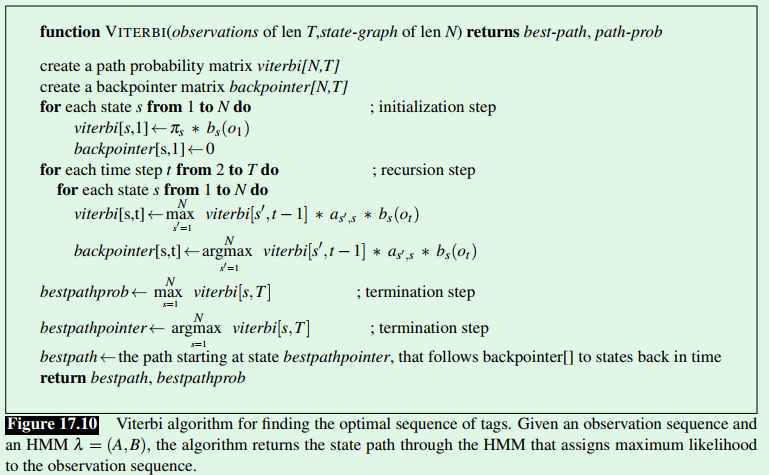
\includegraphics[width=0.8\textwidth]{viterbi.png}
			\caption{Algorithme de Viterbi}
			\label{fig:viterbi} 
		\end{figure}  
	\end{itemize}
	\subsection{Frequence des mots}
	Le modele Frequence des mots represente chaque document d'un corpus sous la forme d'un vecteur de dimension egale a la taille du vocabulaire \footnote{Le vocabulaire est l'ensemble des mots uniques du corpus}. Chaque dimension du vecteur correspond a un mot du vocabulaire, et la valeur associee indique le nombre d'occurences de ce mot dans le document. Il ignore l'ordre des mots.\\
	Supposons que notre corpus est compose des deux phrases suivantes:\\ $P_1=$"Le chat mange le poisson." et $P_2=$"Le poisson nage dans l'eau."\\
	Dans ce cas, notre vocabulaire $V$ est donne par:\\
	\{Le , chat, mange, le, poisson, nage, dans, l', eau \}.\\
	Afin de representer ces deux phrases sous forme vectorielle, on fixe un ordonne les mots du vocabulaire comme suit:\\
	(Le, chat, mange, le, poisson, nage, dans, l', eau).\\
	Ainsi, le vecteur correspondant a $P_1$(respectivement $P_2$) est $(1, 1, 1, 1, 1, 0, 0, 0, 0)$(respectivement $(1, 0, 0, 0, 1, 1, 1, 1, 1)$).
	\subsection{TF-IDF}
	Le TF-IDF est une methode d'extraction de caracteristiques de texte qui evalue l'importance d'un mot dans un document specifique par rapport a son occurence dans l'ensemble du corpus.\\
	$TF\text{-}IDF = TF(t,d) * IDF(t)$\\[2 cm]
	ou:
	\begin{itemize}
	\item $TF(t, d)$ est la frequence d'apparition d'un mot $t$ dans un document $d$ specifique.\\
	$TF(t, d)=\frac{\text{nombre total de mots dans le document } d}{\text{nombre d'occurrences du terme } t \text{ dans le document } d}$
	\item $IDF(t, d)$ reflete l'importance de chaque terme dans un corpus de documents.\\
	$IDF(t)=log(\frac{\text{nombre de documents contenant le terme } t \text{ dans le corpus}}{\text{nombres total de documents dans le corpus}+1})$
	\end{itemize}
	Un TF-IDF eleve indique que le terme est frequent dans le document mais rare dans l'ensemble du corpus.
	\subsection{Skip-gram}
	Skip-gram est une méthode permettant de calculer des embeddings de mots, c’est-à-dire des représentations vectorielles denses et continues des mots.\\
	À partir d’un corpus de documents, le modèle apprend un vecteur pour chaque mot du vocabulaire en entraînant un classificateur binaire. Étant donné une paire $(w,c)$, composée d’un mot cible $w$ et d’un mot candidat $c$, ce classificateur estime la probabilité que $c$ apparaisse dans le contexte de $w$. Les poids appris servent ensuite d’embeddings.\\
	L’algorithme parcourt le corpus et considère chaque mot comme un mot cible. Pour chaque mot cible, il prend en compte ses voisins dans une fenêtre de contexte de taille $L$, qui détermine le nombre de mots à gauche et à droite à considérer.\\
	Par exemple, dans la phrase : « … lemon, a [tablespoon of apricot jam, a] pinch … », si le mot cible est apricot et que $L=2$, les mots de contexte sont tablespoon, of, jam et a.\\
	Skip-gram apprend deux matrices :
	\begin{itemizeFB}
		\item $W$: embedding des mots en tant que cibles.
		\item $C$: embedding des mots en tant que contextes.
	\end{itemizeFB}
	Ces matrices sont initialisées aléatoirement puis ajustées au cours de l’entraînement.\\
	Le modèle skip-gram apprend ainsi deux embeddings distincts pour chaque mot $i$ :
	un embedding cible $w_i$ et un embedding de contexte $c_i$, stockés respectivement dans les matrices $W$ et $C$.
	En pratique, il est courant de combiner ces deux représentations en utilisant la somme $w_i + c_i$ comme embedding final du mot. Alternativement, on peut ne conserver que l’embedding cible $w_i$ et ignorer la matrice $C$.
	Pour chaque paire positive\footnote{Une paire positive est un couple composé de $w$, un mot cible c'est-à-dire le mot que l'on considère, et $c_{pos}$, un vrai mot qui apparaît dans la fenêtre de contexte autour de $w$.} $(w, c_{pos})$, on genere $k$ paires negatives\footnote{Une paire negative est un couple composé de $w$, un mot cible c'est-à-dire le mot que l'on considère, et $c_{neg}$, un mot tiré aléatoirement dans le vocabulaire (différent de $w$).} $(w, c_{neg})$, où $c_{neg}$ est un mot tiré aléatoirement selon une distribution unigramme pondérée :\\
	$P_a(w) = \frac{\text{count}(w)^a}{\sum_{w'} \text{count}(w')^a}$. En pratique, on prend souvent $a=0.75$.\\
	L’objectif est de rapprocher les embeddings des paires positives et d’éloigner ceux des paires négatives.\\
	Pour atteindre cet objectif, les embeddings sont ajustés de manière itérative au cours de l’entraînement. Plus précisément, à chaque étape, les vecteurs sont mis à jour en fonction des paires positives et négatives.\\
	Les équations de mise à jour, de l’instant $t$ à $t+1$, sont données par :
	\[
	c_{pos}^{t+1}=c_{pos}^t-[s(c_{pos}^t.w^t)-1]w^t.
	\]
	\[
	c_{neg}^{t+1}=c_{neg}^t-[s(c_{neg}^t.w^t)]w^t.
	\]
	\[
	w^{t+1}=w^t-([s(c_{pos}^t.w^t-1)]c_{pos}^t+\sum_{i=1}^{k}[s(c_{neg}^t.w^t)]c_{neg}^t).
	\]
	$s(x)$ est la fonction sigmoïde:
	\[
	s(x)=\frac{1}{1+exp(-x)}.
	\]
	\subsection{Régression logistique}
	
	La régression logistique est un classificateur discriminatif\footnote{Un classificateur discriminatif cherche à apprendre à distinguer les classes sans forcément modéliser leur génération.}, probabiliste et supervisé. Elle est utilisée pour classer des données en deux ou plusieurs catégories (par exemple, positif ou négatif). Dans ce cadre, le modèle est entraîné à partir d’un ensemble d’exemples étiquetés $X$, c’est-à-dire que chaque observation $x$ est associée à une étiquette $y$.

	Chaque observation $x$ est décrite par un vecteur de caractéristiques $x = [x_1, ..., x_f]$ où $f$ est le nombre de caractéristiques. Celles-ci peuvent être conçues manuellement ou apprises automatiquement à partir des données, notamment via des méthodes d’apprentissage de représentations ou des gabarits de caractéristiques.

	L’objectif de la régression logistique est de prédire la classe $\hat{y}$ d’une nouvelle observation $x$ à partir de ces caractéristiques. Elle résout cette tâche en apprenant, à partir d’un ensemble d’entraînement, un vecteur de poids $w = [w_1, ..., w_f]$ et un terme de biais $b$. Chaque poids est un nombre réel et est associé à l’une des caractéristiques. Il représente l'importance de cette caractéristique dans la décision de classification.
	
	Comment un classificateur prédit-il la sortie 
	$\hat{y}$ pour une observation $x$ donnée, et comment apprend-il ses paramètres $w$ et $b$ (poids et biais) à partir d’un jeu d’entraînement $X$ ?
	Supposons que $X \in \mathbb{R}^{m \times f}$ (une matrice de taille $m \times f$), où $m$ est le nombre d’observations et $f$ le nombre de caractéristiques. On peut intégrer le biais $b$ dans le vecteur de poids $w$ afin de simplifier les calculs lors de la prédiction et de l’entraînement du modèle. Cela conduit à définir un nouveau vecteur de poids $\tilde{w} \in \mathbb{R}^{f+1}$. Pour ce faire, on ajoute une colonne de $1$ à la matrice $X$, ainsi qu’une composante égale à $1$ à chaque vecteur de caractéristiques $x$. On obtient alors une nouvelle matrice  $\tilde{X} \in \mathbb{R}^{m \times (f+1)}$ et un vecteur $\tilde{x} \in \mathbb{R}^{f+1}$.
	\subsubsection{Cas de la régression logistique binaire}
	
	Le but de la régression logistique binaire est d’entraîner un classificateur capable de prendre une décision binaire à partir d’une observation. Pour une observation donnée, le modèle produit une sortie $ \hat{y} \in [0,1] $, qui représente la probabilité que l’observation appartienne à une classe donnée (classe $0$). Une fois cette probabilité calculée, une décision binaire est obtenue en appliquant un seuil (par exemple 0,5) : si $\hat{y}$ est supérieure à ce seuil, l’observation est classée dans la classe $1$, sinon elle est classée dans la classe $0$.
	
	Pour une observation $x$, le modèle calcule un score:
	\[
	z = \tilde{w} \cdot \tilde{x}
	\]
	Ce score est ensuite transformé en probabilité à l’aide de la fonction sigmoïde :
	\[
	\hat{y} = s(z) = \frac{1}{1+\exp(-z)}
	\]
	La prédiction de la classe est obtenue en appliquant un seuil à $\hat{y}$.
	
	Pour un jeu de données $X$, le modèle calcule un vecteur de scores linéaires :
	\[
	z = \tilde{X} \cdot \tilde{w}^T
	\] 
	où $\tilde{w}^T$ est la tranposée de $w$ et $z$ est un vecteur de taille $m$.\\
	Ces scores sont ensuite transformés en probabilités à l’aide de la fonction sigmoïde appliquée élément par élément :
	
	\[
	\hat{y} = \sigma(z) = [\frac{1}{1 + e^{-z_1}}, ..., \frac{1}{1 + e^{-z_m}}]
	\]
	où $y$ est un vecteur de taille $m$ représentant la probabilité d'appartenance de chaque observation a une classe.\\
	La prédiction de la classe est obtenue en appliquant un seuil (par exemple 0,5) à chaque composante de $\hat{y}$.
	
	Pour que le modèle réalise de bonnes prédictions, il est nécessaire d’apprendre des paramètres adaptés (poids et biais). Pour cela, ces paramètres sont initialisés de manière aléatoire. Ensuite, on mesure l’erreur entre les prédictions $\hat{y}$ et les vraies valeurs $y$ à l’aide d’une fonction de perte. La fonction de perte utilisée pour la régression logistique binaire est la fonction de perte d'entropie croisée:
	\[
	L_{CE}(\hat{y}, y)=-[ylog(s(\tilde{w} \cdot \tilde{x}))+(1-y) log(1-s(\tilde{w} \cdot \tilde{x}))]
	\]
	Cette fonction de perte quantifie l’écart entre les prédictions du modèle et les valeurs réelles. Un algorithme d’optimisation, généralement la descente de gradient, est ensuite utilisé pour minimiser cette perte.Les paramètres sont alors ajustés progressivement de sorte que les prédictions du modèle se rapprochent de plus en plus des valeurs réelles:
	
	\[
	\tilde{w}^{t+1}=\tilde{w}^t - \eta\nabla L(s(\tilde{w} \cdot \tilde{x}), y) 
	\]
	où :
	\begin{itemizeFB}
		\item $L(\hat{y}, y)$ est la fonction de perte qui mesure la proximité entre la prédiction $\hat{y}$ et la vraie valeur $y$.
		\item $\nabla L(\hat{y}, y)$ est le gradient de la fonction de perte par rapport aux paramètres $\tilde{w}$, sachant que $\hat{y} = s(\tilde{w} \cdot \tilde{x})$.
		\item $\tilde{w}^t$ représente la valeur des paramètres à l’itération $t$.
		\item $\eta$ est le taux d’apprentissage.
	\end{itemizeFB}
	
	Comme $\nabla L_{CE}(s(\tilde{w} \cdot \tilde{x}), y) = -(y-\hat{y})\tilde{x}$ alors l'équation ci-dessus devient:
	\[ 
	\tilde{w}^{t+1}=\tilde{w}^t - \eta (s(\tilde{w}^t \cdot \tilde{x}) - y)\tilde{x} 
	\]
	Il existe plusieurs façons de calculer cette cette mise à jour:
	
	\begin{itemizeFB}
		\item \textbf{Stochastique} : elle sélectionne un seul exemple aléatoire $x$ à chaque itération. Puis elle ajuste les paramètres :
		\[ 
		\tilde{w}^{t+1}=\tilde{w}^t - \eta (s(\tilde{w}^t \cdot \tilde{x}) - y)\tilde{x} 
		\]
		\item \textbf{Par lots} : elle utilise tout le jeu d’entraînement pour calculer une seule mise à jour des paramètres.
		\item \textbf{Par mini-lots} : elle utilise un sous-ensemble $X'$ de $\tilde{X}$, de taille $n$, pour calculer une seule mise à jour des paramètres:
		\[
		\tilde{w}^{t+1}=\tilde{w}^t - \eta X'^T(s(X' \cdot (\tilde{w}^t)^T) - y) 
		\]
		où $(\tilde{w}^t)^T$ (resp. $X'^T$) est la transposée de $(\tilde{w}^t)$ (resp. $X'$) 
	\end{itemizeFB}
	
\subsubsection{Régression logistique multinomiale}

La régression logistique multinomiale permet de réaliser une classification avec plus de deux classes.

Étant donné un jeu de données étiqueté $X$, soit $ \mathcal{K} $ l’ensemble des classes possibles et $ K = |\mathcal{K}| $ leur nombre. Pour chaque observation $ x $, l’étiquette correcte $y$ est représentée par un vecteur one-hot\footnote{Un vecteur one-hot est un vecteur contenant un seul élément égal à 1 et tous les autres égaux à 0.} de taille $K$. Si la classe correcte est $c$, alors $ y_c = 1 $ et $ y_k = 0 $ pour tout $ k \neq c $.

Le classificateur prend en entrée une observation $x$ et produit en sortie un vecteur $\hat{y} \in \mathbb{R}^K$. Chaque composante $\hat{y}_k$ représente la probabilité que l’observation appartienne à la classe $k$, avec :
\[
\sum_{k=1}^{K} \hat{y}_k = 1.
\]

Dans la régression logistique multinomiale, on associe à chaque classe $k$ un vecteur de poids $w_k \in \mathbb{R}^f$ et un biais $b_k$. Ces paramètres peuvent être regroupés sous forme matricielle dans une matrice $W \in \mathbb{R}^{K \times f}$ et un vecteur de biais $b \in \mathbb{R}^K$, afin de simplifier les calculs.

Afin de simplifier les calculs, le biais $b$ est intégré dans la matrice des poids $W$ ce qui nous donne une nouvelle matrice $\tilde{W} \in \mathbb{R}^{K \times (f+1)}$.
	
Pour une observation $x$, le modèle calcule un score:

\[
z = \tilde W \cdot \tilde{x}^T
\]

La prédiction est ensuite donnée par :
\[
\hat{y} = \text{softmax}(z)
\]

où :
\[
	\text{softmax}(z) = [\frac{\exp(z_1)}{\sum_{j=1}^{K} \exp(z_j)}, ..., \frac{\exp(z_K)}{\sum_{j=1}^{K} \exp(z_j)}]
\]
Chaque composante de $\hat{y}$ est comprise entre 0 et 1, et la somme des composantes du vecteur est égale à 1.
Chaque composante $k$ de $\hat{y}$ représente la probabilité que l’observation $x$ appartienne à la classe $k$.
	

Pour un jeu de données $X$, on calcule alors les prédictions de tous les observations en une seule opération:

\[
Z = \tilde{X} \cdot \tilde{W}^T
\]

où $\tilde{W}^T$ est la transposée de $\tilde{W}$

Ensuite, on applique la fonction softmax ligne par ligne sur $Z$ pour obtenir :

\[
\hat{Y} = \text{softmax}(Z)
\]

où $\hat{Y} \in \mathbb{R}^{m \times K}$, contenant pour chaque exemple une distribution de probabilité sur les classes.

Comment les poids sont-ils appris ?\\

La fonction d’entropie croisée, utilisée pour mesurer l’écart entre la valeur prédite $\hat{y}$ par le modèle et la valeur réelle $y$, en régression logistique multinomiale pour une observation $\tilde{x}$ de $\tilde{X}$, est donnée par :

\[
L_{CE}(\hat{y}, y)
= - \sum_{i=1}^{K} y_i \log \hat{y}_i
= - \log \hat{y}_k
= - \log \left(
\frac{\exp(\tilde{w}_k \cdot \tilde{x})}
{\sum_{i=1}^{K} \exp(\tilde{w}_i \cdot \tilde{x})}
\right)
\]

où $k$ est la classe correcte et $\tilde{w}_k$ représente les paramètres (poids et biais) associés à la classe $k$.\\

La fonction d’entropie croisée, utilisée pour mesurer l’écart entre les prédictions $\hat{Y}$ du modèle et les valeurs réelles $Y$, en régression logistique multinomiale sur l’ensemble du jeu d’entraînement $\tilde{X}$, est donnée par :

\[
L_{CE}(\hat{Y}, Y)
= - \frac{1}{m} \sum_{i=1}^{m} \sum_{j=1}^{K} y_j^{(i)} \log \hat{y}_j^{(i)}
\]

où :
\begin{itemize}
	\item $\hat{Y} \in \mathbb{R}^{m \times K}$ est la matrice des prédictions ; chaque ligne $i$ de $\hat{Y}$ correspond à une distribution de probabilités sur les $K$ classes pour l’exemple $\tilde{x}^{(i)}$.
	\item $Y \in \mathbb{R}^{m \times K}$ est la matrice des étiquettes réelles ; chaque ligne $i$ de $Y$ est un vecteur one-hot représentant la classe réelle de l’exemple $\tilde{x}^{(i)}$.
	\item $y_j^{(i)}$ est la $j$-ème composante du vecteur cible $y^{(i)}$.
	\item $\hat{y}_j^{(i)}$ est la probabilité prédite par le modèle pour la classe $j$ et l’exemple $i$.
\end{itemize}
On utilise ensuite un algorithme de descente de gradient pour minimiser cette fonction de perte.

Pour chaque classe $k$, le gradient de l’entropie croisée par rapport au vecteur de paramètres $\tilde{w}_k$ est donné par :
\[
\nabla_{\tilde{w}_k} L_{CE}(\hat{Y}, Y)
= \frac{1}{m} \sum_{i=1}^{m} \big(\hat{y}_k^{(i)} - y_k^{(i)}\big)\, \tilde{x}^{(i)}
\]

où :
\begin{itemize}
	\item $\hat{y}_k^{(i)}$ est la probabilité prédite par le modèle pour la classe $k$ et l’exemple $i$.
	\item $y_k^{(i)}$ est la valeur réelle (étiquette) pour la classe $k$ et l’exemple $i$ (issue d’un encodage one-hot).
	\item $\tilde{x}^{(i)}$ est le vecteur de caractéristiques de l’exemple $i$, éventuellement augmenté pour inclure le biais.
\end{itemize}

Les paramètres sont ensuite mis à jour selon la règle de descente de gradient :
\[
\tilde{w}_k^{(t+1)}
= \tilde{w}_k^{(t)}
- \eta \, \frac{1}{m} \sum_{i=1}^{m} \big(\hat{y}_k^{(i)} - y_k^{(i)}\big)\, \tilde{x}^{(i)}
\]

où :
\begin{itemize}
	\item $\tilde{w}_k^{(t)}$ est le vecteur de paramètres de la classe $k$ à l’itération $t$.
	\item $\tilde{w}_k^{(t+1)}$ est le vecteur de paramètres mis à jour après l’itération $t$.
	\item $\eta$ est le taux d’apprentissage.
\end{itemize}

\subsection{Réseaux de neuronnes récurrents}
Les réseaux de neurones sont une approche d’apprentissage automatique inspirée du fonctionnement des neurones biologiques du cerveau humain. Ils apprennent à partir de données et peuvent être utilisés pour des tâches de classification, de régression ou de prédiction. Ils sont particulièrement adaptés à la modélisation de relations non linéaires complexes.

Un réseau de neurones artificiel est généralement composé d’une couche d’entrée, d’une ou plusieurs couches cachées et d’une couche de sortie. La profondeur d’un réseau correspond au nombre de couches de neurones qu’il contient ; la couche d’entrée n’est généralement pas comptée dans ce nombre. Chaque couche est composée d’un certain nombre d’unités appelées neurones artificiels. Le nombre de neurones d’une couche correspond à la taille de cette couche. La taille de la couche d’entrée est égale à la dimension du vecteur d’entrée $x$.

Dans un réseau de neurones classique entièrement connecté, les neurones d’une même couche ne sont généralement pas connectés entre eux. Les connexions se font entre couches successives : chaque neurone d’une couche est relié à tous les neurones de la couche suivante.

Chaque neurone d’une couche cachée ou de sortie reçoit en entrée un vecteur de valeurs réelles $x$, associé à un vecteur de poids $w$, ainsi qu’un biais $b$, généralement un scalaire. Le neurone calcule d’abord une combinaison linéaire :
\[
z=w \cdot x + b
\]
Puis une fonction d’activation non linéaire $f$ est appliquée afin d’obtenir la sortie du neurone :
\[
y=f(z)
\]
Cette fonction d’activation peut être, par exemple, la fonction sigmoïde, la tangente hyperbolique (tanh) ou la fonction ReLU (Rectified Linear Unit). La sortie d’une couche est donc un vecteur contenant les sorties de tous ses neurones.

Lorsqu’une entrée x est fournie au réseau, l’information se propage de la couche d’entrée vers les couches cachées puis vers la couche de sortie. Afin de simplifier les calculs, les poids des neurones d’une même couche sont regroupés dans une matrice de poids, et les biais dans un vecteur de biais. Ces paramètres sont initialisés aléatoirement puis ajustés pendant l’entraînement afin de minimiser l’erreur du modèle.

Un réseau de neurones récurrent est tout réseau de neurones qui contient un cycle dans ses connexions internes ce qui signifie que la valeur d’une certaine unite neuronale depend directement ou indirectement de ses propres sorties precedentes comme entree.\cite{RNN1}. Grâce à cette propriété, les RNN sont capables de conserver une information sur le contexte précédent. Ils sont donc particulièrement adaptés au traitement de données séquentielles telles que les séries temporelles, le texte, la parole ou les séquences biologiques.

Pour comprendre le fonctionnement des RNN, considérons le cas d’un RNN simple, c’est-à-dire un réseau récurrent qui associe une séquence d’entrée à une séquence de sortie de même longueur. Les éléments de la séquence sont traités un à un, dans l’ordre.\\
La figure  ~\ref{fig:Structure de la RNN simple} illustre la structure de ce réseau.

\begin{figure}[H]
	\centering
	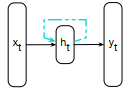
\includegraphics[width=0.175\textwidth]{structureRNN.png}
	\caption{Structure de la RNN simple}
	\label{fig:Structure de la RNN simple} 
\end{figure}

L’indice t représente le temps ou la position dans la séquence.\\
À chaque instant t :
\begin{itemizeFB}
	\item $x^{(t)}$ représente l’entrée du réseau ;
	\item $h^{(t)}$ représente la couche caché du réseau ;
	\item $y^{(t)}$ représente la sortie du réseau.
\end{itemizeFB}
La couche cachée $h^{(t)}$ dépend à la fois de l'entrée actuelle $x^{(t)}$ et de la couche cachée précédente $h^{(t-1)}$. Ainsi, la couche caché $h(t)$ influence donc directement la valeur de la sortie $y^{(t)}$ et indirectement les valeurs des couches cachees futures et sorties futures .

Le réseau récurrent peut être représenté sous deux formes :
\begin{itemizeFB}
	\item une représentation compacte avec une boucle récurrente ;
	\item une représentation déroulée dans le temps, où chaque instant de temps est représenté explicitement.
\end{itemizeFB}
Le déroulement du réseau est particulièrement utile pour appliquer l’algorithme de rétropropagation à travers le temps (Backpropagation Through Time ou BPTT), utilisé pour calculer les gradients et mettre à jour les poids.
Ces deux représentations sont illustrées dans la figure ~\ref{fig: Deux représentations de la RNN simple}.
\begin{figure}[H]
	\centering
	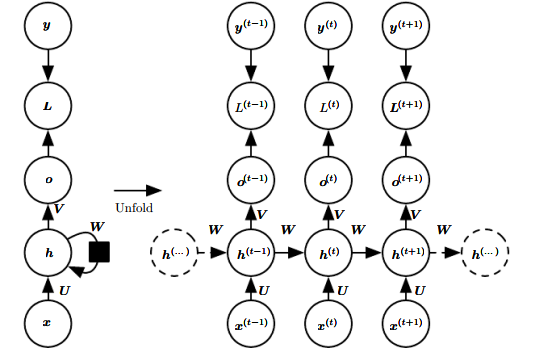
\includegraphics[width=0.7\textwidth]{RNNRepresentation.png}
	\caption{La figure à gauche est une représentation compacte de la RNN simple et celle à droite est sa représentation déroulée dans le temps }
	\label{fig: Deux représentations de la RNN simple} 
\end{figure}

D'après la figure ci-dessus, dans un RNN simple, le passage d’une séquence d’entrées à une séquence de sorties se fait de la manière suivante.\\
La matrice $U$ relie l’entrée à la couche cachée, la matrice $W$ relie l’état caché précédent à l’état caché courant, et la matrice $V$ relie la couche cachée à la couche de sortie. Les mêmes matrices de poids sont utilisées à chaque instant de temps.
Le calcul commence par l’initialisation de l’état caché initial, souvent :
\[
h^{(0)}=0
\] 
Ensuite, pour chaque instant $t$ allant de $1$ à $T$, où $T$ est la longueur de la séquence, les calculs suivants sont effectués :
\[
a^{(t)}=b + W \cdot h^{(t-1)} + U \cdot x^{(t)}
\]
\[
h^{(t)}=f(a^{(t)})
\]
\[
o^{(t)}=V \cdot h^{(t)} + c
\]
\[
y^{(t)}=g(o^{(t)})
\]
où:
\begin{itemizeFB}
	\item $f$ est la fonction d'activation non lineaire de la couche cachée.
	\item $g$ est la fonction d'activation non lineaire de la couche de sortie.
	\item $b$ est le vecteur de biais de la couche cachée.
	\item $c$ est le vecteur de biais de la couche de sortie.
\end{itemizeFB}
La séquence $y$ est composé des $y^{(t)}$ pour t allant de $1$ jusqu'à $T$.

L’objectif de l’entraînement est d’apprendre les matrices de poids W, U et V ainsi que les biais b et c. Pour cela, on utilise :
\begin{itemizeFB}
	\item un jeu de données d’entraînement ;
	\item une fonction de perte permettant de mesurer l’écart entre les prédictions du modèle et les valeurs réelles.
\end{itemizeFB}
L’entraînement d’un réseau de neurones récurrent (RNN) se déroule généralement en deux étapes : la propagation avant et la rétropropagation à travers le temps.\\

La première étape, appelée propagation avant, consiste à faire passer chaque séquence d’entrée dans le réseau afin de calculer les sorties prédites. À chaque instant $t$, une perte locale $L^{(t)}$ est calculée en comparant la sortie prédite à la sortie réelle. La perte totale associée à une séquence est ensuite obtenue en additionnant les pertes sur tous les instants :

\[
L = \sum_{t=1}^{T} L^{(t)}
\]

où $T$ désigne la longueur de la séquence.\\

La deuxième étape consiste à calculer les gradients de la perte totale par rapport aux paramètres du réseau ($W$, $U$, $V$, $b$ et $c$). Ces gradients indiquent comment modifier les paramètres afin de réduire l’erreur du modèle.\\

Afin de faciliter le calcul des gradients, le réseau est déroulé dans le temps pour former un graphe computationnel. Cette représentation permet d’appliquer l’algorithme de rétropropagation à travers le temps.\\

Dans le graphe computationnel déroulé, les nœuds incluent les paramètres du réseau ($W$, $U$, $V$, $b$ et $c$) ainsi que les variables dépendant du temps : $x^{(t)}$, $h^{(t)}$, $o^{(t)}$ et $L^{(t)}$.\\

Le calcul des gradients commence par les nœuds les plus proches de la fonction de perte. On calcule d’abord le gradient de la perte totale $L$ par rapport à chaque perte locale $L^{(t)}$ :

\[
\frac{\partial L}{\partial L^{(t)}} = 1
\]

Ensuite, on calcule le gradient de $L$ par rapport à la sortie $o^{(t)}$ pour chaque instant $t$ :

\[
\nabla_{o^{(t)}} L = \frac{\partial L}{\partial L^{(t)}}
\frac{\partial L^{(t)}}{\partial o^{(t)}}
\]

Au dernier instant $T$, l’état caché $h^{(T)}$ influence uniquement la sortie $o^{(T)}$. Son gradient est donc donné par :

\[
\nabla_{h^{(T)}} L = V^\top \nabla_{o^{(T)}} L
\]

Pour les instants précédents, chaque état caché $h^{(t)}$ influence à la fois la sortie courante $o^{(t)}$ et l’état caché suivant $h^{(t+1)}$. Le gradient doit donc être propagé à travers ces deux dépendances.\\

On itère ainsi de $t=T-1$ jusqu’à $t=1$ afin de calculer récursivement le gradient par rapport à chaque état caché :

\[
\nabla_{h^{(t)}} L=\left(\frac{\partial h^{(t+1)}}{\partial h^{(t)}}\right)^\top \nabla_{h^{(t+1)}} L + \left(\frac{\partial o^{(t)}}{\partial h^{(t)}}\right)^\top \nabla_{o^{(t)}} L
\]

Une fois les gradients calculés sur les nœuds internes du graphe computationnel, on peut calculer les gradients par rapport aux paramètres du réseau.\\

Le gradient par rapport au biais de sortie $c$ est donné par :

\[
\nabla_c L
=\sum_t \left(\frac{\partial o^{(t)}}{\partial c}\right)^\top \nabla_{o^{(t)}} L
\]

Le gradient par rapport au biais caché $b$ est :

\[
\nabla_b L
=\sum_t \left(\frac{\partial h^{(t)}}{\partial b} \right)^\top \nabla_{h^{(t)}} L
\]

Le gradient par rapport à la matrice de poids $V$ est :

\[
\nabla_V L
=\sum_t (\nabla_{o^{(t)}} L) (h^{(t)})^\top
\]

Le gradient par rapport à la matrice récurrente $W$ est :

\[
\nabla_W L
=\sum_t \sum_i \frac{\partial L}{\partial h_i^{(t)}} \nabla_{W^{(t)}} h_i^{(t)}
\]

Le gradient par rapport à la matrice d’entrée $U$ est :

\[
\nabla_U L
=\sum_t \sum_i \frac{\partial L}{\partial h_i^{(t)}} \nabla_{U^{(t)}} h_i^{(t)}
\]

Les gradients calculés sont ensuite utilisés pour mettre à jour les paramètres du réseau à l’aide d’un algorithme d’optimisation basé sur le gradient, comme la descente de gradient.\\

À l’itération $i+1$, les paramètres sont mis à jour selon les équations suivantes :

\[
c^{(i+1)} = c^{(i)} - \eta \nabla_c L
\]
\[
b^{(i+1)} = b^{(i)} - \eta \nabla_b L
\]
\[
V^{(i+1)} = V^{(i)} - \eta \nabla_V L
\]
\[
W^{(i+1)} = W^{(i)} - \eta \nabla_W L
\]
\[
U^{(i+1)} = U^{(i)} - \eta \nabla_U L
\]

où $\eta$ désigne le taux d’apprentissage.
	
	
	\chapter{Byte Pair Encoding}
	
	Le Byte Pair Encoding (BPE) est une technique de compression de données consistant à fusionner itérativement les paires d’octets ou de caractères consécutifs les plus fréquentes d’un texte ou d’une séquence de données en un nouveau symbole unique. Le processus est répété jusqu’à atteindre un nombre prédéfini de fusions ou jusqu’à ce qu’il ne reste plus de paires fréquentes.
	
	Cette méthode a été décrite pour la première fois en 1994 par Philip Gage. Elle est ensuite devenue l’une des techniques de tokenisation en sous-mots les plus utilisées en traitement automatique du langage naturel (TALN).
	
	\section{Présentation}
	
	L’idée de l’algorithme est de représenter les paires les plus fréquentes par des marqueurs dédiés. Ce faisant, il identifie les séquences d’éléments (caractères) les plus fréquentes. Ensuite, en utilisant ces informations, il peut encoder des textes.
	\subsection{Logique principale}
	La logique de l’algorithme est illustrée par les étapes suivantes :
	
	\begin{enumerate}
		\item Construire un vocabulaire à partir d’un corpus de mots.
		
		\item Identifier la paire la plus fréquente : compter les paires de symboles et sélectionner celle ayant la fréquence la plus élevée.
		
		\item Produire un nouvel élément de vocabulaire pour la paire la plus fréquente : fusionner cette paire en un nouveau symbole et mettre à jour le corpus afin de refléter ce nouvel élément.
		
		\item Répéter les étapes précédentes jusqu’à atteindre un nombre cible de fusions.
		
		\item Enregistrer la table des fusions.
		
		\item Encoder une chaîne de caractères à l’aide de la table des fusions.
	\end{enumerate}
	
\subsection{Illustration à travers un exemple}

	\begin{verbatim}
		b := BytePairEncoder new.
		b fromText: 'FRED FED TED BREAD, AND TED FED FRED BREAD'.
	\end{verbatim}
	
\textbf{Inspection du corpus}

Tout d’abord, une fois le texte d’entrée tokenisé, on obtient le vocabulaire suivant.

	\begin{verbatim}
		corpus  
			#('F' 'E' 'D' '_') 2
			#('B' 'R' 'E' 'A' 'D' '_') 2
			#('A' 'N' 'D' '_') 1
			#('T' 'E' 'D' '_') 2
			#('F' 'R' 'E' 'D' '_') 2
	\end{verbatim}
	
Lorsque l’on observe le système, on obtient les éléments suivants :

\begin{itemize}
	\item un vocabulaire : \texttt{'T' 'A' 'F' 'D' 'B' '\_' 'R' 'N' 'E'}
	\item un corpus : comme indiqué ci-dessus
	\item une liste de paires consécutives avec leurs fréquences
	\item une liste de fusions vide
\end{itemize}

\begin{verbatim}
	voc  
		'T' 'A' 'F' 'D' 'B' '_' 'R' 'N' 'E'
	corpus  
		#('F' 'E' 'D' '_') 2
		#('B' 'R' 'E' 'A' 'D' '_') 2
		#('A' 'N' 'D' '_') 1
		#('T' 'E' 'D' '_') 2
		#('F' 'R' 'E' 'D' '_') 2
	pairs  
		#('N' 'D') 1
		#('B' 'R') 2
		#('A' 'N') 1
		#('A' 'D') 2
		#('F' 'E') 2
		#('D' '_') 9
		#('R' 'E') 4
		#('E' 'A') 2
		#('T' 'E') 2
		#('E' 'D') 6
		#('F' 'R') 2
	merges 
\end{verbatim}

On observe que la paire la plus fréquente est \texttt{\#('A'~'B')}. Elle sera donc celle qui sera fusionnée.\\

\textbf{Itération 1}

Maintenant, examinons la situation avec la première fusion.

\begin{verbatim}
b mergeOneStep
\end{verbatim}

On observe que la paire la plus fréquente \texttt{\#('D'~'\_')} a été fusionnée. Cela signifie que :

\begin{itemizeFB}
	
	\item Elle a été ajoutée au vocabulaire : ici, nous obtenons par exemple \texttt{'D\_'} comme nouvel élément. À noter que si les caractères étaient encodés par des nombres, les éléments fusionnés seraient simplement représentés par un nouvel identifiant numérique.
	
	\item Elle a été ajoutée à la liste des fusions.
	
	\item Le corpus a été mis à jour afin de refléter la présence du nouvel élément du vocabulaire. Par exemple, \texttt{\#('F' 'E' 'D' '\_')} est désormais encodé comme \texttt{\#('F' 'E' 'D\_')}.
	
	\item Toutes les paires ont été recalculées à partir de la version mise à jour du corpus. Ainsi, la paire la plus fréquente devient maintenant \texttt{\#('E' 'D\_')}.
	
\end{itemizeFB}

\begin{verbatim}
voc  
	'F' 'R' 'T' 'B' 'N' 'D_' '_' 'E' 'D' 'A'
corpus  
	#('F' 'E' 'D_') 2
	#('A' 'N' 'D_') 1
	#('B' 'R' 'E' 'A' 'D_') 2
	#('T' 'E' 'D_') 2
	#('F' 'R' 'E' 'D_') 2
pairs  
	#('E' 'D_') 6
	#('B' 'R') 2
	#('A' 'N') 1
	#('N' 'D_') 1
	#('F' 'E') 2
	#('E' 'A') 2
	#('R' 'E') 4
	#('T' 'E') 2
	#('F' 'R') 2
	#('A' 'D_') 2
merges 
	#('D' '_')->'D_'	
\end{verbatim}

\textbf{Itération 2}

L’algorithme répète le même processus. Ainsi, la fusion \texttt{\#('E' 'D\_') → 'ED\_'} est ajoutée à la liste des fusions. Le vocabulaire, le corpus et les paires sont ensuite mis à jour.

\begin{verbatim}
	
voc  
	'F' 'R' 'ED_' 'T' 'B' 'N' 'D_' '_' 'E' 'D' 'A'
corpus  
	#('T' 'ED_') 2
	#('F' 'R' 'ED_') 2
	#('A' 'N' 'D_') 1
	#('B' 'R' 'E' 'A' 'D_') 2
	#('F' 'ED_') 2
pairs  
	#('T' 'ED_') 2
	#('B' 'R') 2
	#('A' 'N') 1
	#('N' 'D_') 1
	#('R' 'E') 2
	#('E' 'A') 2
	#('F' 'R') 2
	#('A' 'D_') 2
	#('R' 'ED_') 2
	#('F' 'ED_') 2
merges 
	#('D' '_')->'D_'
	#('E' 'D_')->'ED_'
\end{verbatim}

On observe maintenant qu’il existe plusieurs paires ayant la fréquence la plus élevée. L’algorithme en sélectionnera une parmi elles.\\

\textbf{Itération 3}

Voici l’itération suivante. La fusion \texttt{\#('T' 'ED\_')} $\rightarrow$ \texttt{'TED\_'} a été ajoutée à la liste des fusions. Il est à noter qu’il s’agit de la première paire apparaissant dans le journal présenté ici, mais cela est simplement dû au fait que la logique d’affichage utilise la même implémentation de type \textit{bag} ainsi que la même logique de tri que celle utilisée par l’algorithme lorsqu’il recherche l’association la plus fréquente. Cela n’est pas lié à l’algorithme lui-même. Une autre paire ayant la même fréquence aurait pu être sélectionnée.

\begin{verbatim}
voc  
	'F' 'R' 'ED_' 'T' 'B' 'N' 'D_' '_' 'E' 'TED_' 'D' 'A'
corpus  
	#('F' 'R' 'ED_') 2
	#('A' 'N' 'D_') 1
	#('B' 'R' 'E' 'A' 'D_') 2
	#('TED_') 2
	#('F' 'ED_') 2
	pairs  
	#('B' 'R') 2
	#('A' 'N') 1
	#('N' 'D_') 1
	#('R' 'E') 2
	#('E' 'A') 2
	#('F' 'R') 2
	#('A' 'D_') 2
	#('R' 'ED_') 2
	#('F' 'ED_') 2
merges 
	#('D' '_')->'D_'
	#('E' 'D_')->'ED_'
	#('T' 'ED_')->'TED_'
\end{verbatim}

\textbf{Itération 4}
Voici une autre itération au cours de laquelle la paire \texttt{\#('B' 'R')} a été sélectionnée.

\begin{verbatim}
	voc  
		'BR' 'F' 'R' 'ED_' 'T' 'B' 'N' 'D_' '_' 'E' 'TED_' 'D' 'A'
	corpus  
		#('F' 'R' 'ED_') 2
		#('F' 'ED_') 2
		#('A' 'N' 'D_') 1
		#('TED_') 2
		#('BR' 'E' 'A' 'D_') 2
		pairs  
		#('BR' 'E') 2
		#('A' 'N') 1
		#('N' 'D_') 1
		#('E' 'A') 2
		#('F' 'R') 2
		#('F' 'ED_') 2
		#('R' 'ED_') 2
		#('A' 'D_') 2
	merges 
		#('D' '_')->'D_'
		#('E' 'D_')->'ED_'
		#('T' 'ED_')->'TED_'
		#('B' 'R')->'BR'
\end{verbatim}

\textbf{Jusqu’à ce qu’aucune fusion supplémentaire ne soit possible.}\\
L’algorithme continue comme expliqué jusqu’à ce qu’il n’y ait plus de paires à fusionner, c’est-à-dire lorsque la fréquence des paires est égale à un. On obtient la situation suivante.

\begin{verbatim}
	oc  
		'BR' 'BREA' 'R' 'TED_' 'ED_' 'E' 'N' 'FR' 'A' 'BRE' '_' 'F' 'D_' 'BREAD_' 'D' 'FRED_' 'FED_' 'T' 'B'
	corpus  
		#('FRED_') 2
		#('FED_') 2
		#('BREAD_') 2
		#('A' 'N' 'D_') 1
		#('TED_') 2
	pairs  
		#('A' 'N') 1
		#('N' 'D_') 1
	merges 
		#('D' '_')->'D_'
		#('E' 'D_')->'ED_'
		#('T' 'ED_')->'TED_'
		#('B' 'R')->'BR'
		#('BR' 'E')->'BRE'
		#('BRE' 'A')->'BREA'
		#('F' 'R')->'FR'
		#('BREA' 'D_')->'BREAD_'
		#('F' 'ED_')->'FED_'
		#('FR' 'ED_')->'FRED_'
\end{verbatim}

\textbf{Utilisation des fusions}

Nous pouvons maintenant encoder un texte. La logique de cette étape est la suivante :

\begin{itemizeFB}
	\item tokeniser le texte ;
	\item parcourir la liste des fusions dans l’ordre et appliquer chaque fusion l’une après l’autre sur le résultat de l’application précédente ;
	\item une fois arrivé à la fin de la liste des fusions, on obtient le texte encodé.
\end{itemizeFB}

Imaginons que nous voulions encoder \texttt{'FRED EATS BREAD'}. Lors de la phase de tokenisation, nous obtenons la liste suivante:

\begin{verbatim}
	'F' 'R' 'E' 'D' '_' 'E' 'A' 'T' 'S' '_' 'B' 'R' 'E' 'A' 'D_'
\end{verbatim}

À noter que l’on pourrait également travailler au niveau des mots et utiliser une structure de type Bag afin de factoriser le traitement pour des mots similaires.\\
Ensuite, nous demandons à l’algorithme d’encoder le texte. On obtient la liste d’éléments suivante : \texttt{‘FRED\_’ ‘E’ ‘A’ ‘T’ ‘S’ ‘’ ‘BREAD’}

\begin{verbatim}
	self encode: 'FRED EATS BREAD' 
	> an OrderedCollection('FRED_' 'E' 'A' 'T' 'S' '_' 'BREAD_')
\end{verbatim}

Ce que l’on observe, c’est que les mots fréquents ont été substitués. Ainsi, si on l’examine sous une forme numérique, on obtient :

\begin{verbatim}
	'ABRC' asArray collect: [ :each | each digitValue -9 ]
	>  #(1 2 18 3)

	'FRED EATS BREAD' asArray collect: [ :each | each digitValue -9 ] 
	> #(6 18 5 4 -10 5 1 20 19 -10 2 18 5 1 4)

	'EATS_' asArray collect: [ :each | each digitValue -9 ] 
	> #(5 1 20 19 -10) 
\end{verbatim}

Par conséquent, le texte passe de $15$ à $7$ éléments (car ‘FRED\_’ et ‘BREAD\_’ comptent chacun comme un seul élément).

\subsection{Observation sur l'algorithme}

L’exécution que nous avons présentée correspond à une implémentation naïve et simple. Elle reconstruit l’ensemble complet des paires à chaque itération. De plus, une seule paire est fusionnée à la fois.\\
Ce que montre cette exécution, c’est que le vocabulaire, le corpus et les paires doivent être mis à jour à chaque fusion.\\
Plusieurs paires pourraient être fusionnées au cours d’un même passage si l’algorithme prend en compte le fait que les paires fusionnées simultanément ne doivent ni commencer ni se terminer par un élément similaire.\\
Lorsque l’on dispose des paires suivantes :

\begin{verbatim}
	#('N' 'D') 1
	#('B' 'R') 2
	#('A' 'N') 1
	#('A' 'D') 2
	#('F' 'E') 2
	#('D' '_') 9
	#('R' 'E') 4
	#('E' 'A') 2
	#('T' 'E') 2
	#('E' 'D') 6
	#('F' 'R') 2
\end{verbatim}

Lors de la fusion de \texttt{\#('D' '') 9}, l’algorithme ne devrait pas fusionner les paires se terminant par ‘D’ ou commençant par ‘\_’, mais il pourrait en fusionner d’autres, comme ‘R’ ‘E’. Or, la fusion simultanée de plusieurs paires conduit à des encodages différents.

\section{Implémentation}

L'objectif cette section est d'implémenter l'algorithme Byte Pair Encoding (BPE) en Pharo.
Le fonctionnement de BPE est décrit la section \textbf{1.3.1.1}.

\subsection{Algorithme pseudo-code}

\textbf{L’algorithme 1} prend en entrée un texte ainsi que le nombre de fusions souhaité ou la taille du vocabulaire souhaitée. Il permet l’entraînement de l’algorithme BPE sur le texte donné en entrée et retourne :

\begin{itemizeFB}
	\item un dictionnaire des fusions ;
	\item ainsi que le vocabulaire appris.
\end{itemizeFB}

Le dictionnaire des fusions contient :

\begin{itemizeFB}
	\item comme clés, les nouveaux symboles créés lors des différentes opérations de fusion ;
	\item et comme valeurs, l’ordre dans lequel ces symboles ont été appris pendant l’entraînement.
\end{itemizeFB}

L’algorithme commence par initialiser le vocabulaire à l’aide de la fonction \texttt{InitializeVocabulary()}. Cette fonction construit l’ensemble des symboles présents dans le texte d’entrée. Le vocabulaire contient également le symbole spécial '\_', utilisé pour indiquer la fin d’un mot dans BPE.

Ensuite, la fonction \texttt{ComputeWordsFrequencies()} calcule la fréquence de chaque mot du texte tout en transformant chaque mot en une liste de caractères. Les mots prétraités ainsi que leurs fréquences sont ensuite enregistrés dans un dictionnaire représentant le corpus.

Après cette étape, l’algorithme effectue zéro, une ou plusieurs itérations jusqu’à ce que le nombre de fusions souhaité la taille du vocabulaire souhaitée soit atteint.

À chaque itération :

\begin{itemizeFB}
    \item les fréquences des paires de symboles consécutifs présentes dans le corpus sont calculées à l’aide de la fonction \texttt{ComputePairs()} ;
	\item la paire possédant la fréquence maximale est ensuite sélectionnée ;
	\item les deux symboles composant cette paire sont fusionnés afin de créer un nouveau symbole.
	\item le nouveau symbole obtenu est ajouté au dictionnaire des fusions, où la valeur associée correspond au numéro de l’itération courante, ainsi qu’au vocabulaire.
	\item le corpus est mis à jour à l’aide de la fonction \texttt{UpdateCorpus()}, qui remplace toutes les occurrences de la paire sélectionnée par le nouveau symbole fusionné.
\end{itemizeFB}

\begin{algorithm}[H]
	\caption{TrainBPE}
	\KwIn{text, mergeCount}
	\KwOut{mergesDictionary, vocabulary}
	
	vocabulary $\leftarrow$ InitializeVocabulary(text)\;
	
	$corpus \leftarrow$ computeWordsFrequency(text)\;
	
	mergesDictionary $\leftarrow$ empty dictionary\;
	
	$i \leftarrow$ mergeCount - Size(vocabulary)\;
		
	$j \leftarrow 1$\;
		
	\While{$i>0$}{
			$pairs \leftarrow$ ComputePairs($corpus$)\;
			
			$bestPair \leftarrow$ Max($pairs$)\;
			
			$newSymbol \leftarrow bestPair[1] + bestPair[2]$\;
			
			mergesDictionary[$newSymbol$] $\leftarrow j$\;
			
			Add(vocabulary, $newSymbol$)\;
			
			$corpus \leftarrow$ UpdateCorpus($corpus$, $bestPair$, $newSymbol$)\;
			
			$j = j + 1$\;
			
			$i \leftarrow i - 1$\;
		}
	\Return{mergesDictionary, vocabulary}
\end{algorithm}

\vspace{0.5cm}

\textbf{L’algorithme 2} prend en entrée un texte et retourne un dictionnaire représentant le texte prétraité. Dans ce dictionnaire :

\begin{itemizeFB}
	\item les clés correspondent à des listes de caractères représentant les mots du corpus ;
	\item les valeurs correspondent aux fréquences d’apparition de ces mots dans le texte.
\end{itemizeFB}

L’algorithme parcourt le texte caractère par caractère afin d’identifier les mots. Chaque mot représenté sous forme d’une liste de caractères représentant sa décomposition initiale utilisée par BPE.

L’espace joue le rôle de séparateur de mots. Lorsqu’un espace est rencontré pendant le parcours du texte, l’algorithme considère que le mot courant est terminé. La liste de caractères construite jusqu’à ce point est alors ajoutée au dictionnaire, puis une nouvelle liste est initialisée pour traiter le mot suivant.

De manière générale, les espaces ainsi que les signes de ponctuation peuvent être utilisés comme séparateurs de mots lors du prétraitement d'un texte. Toutefois, dans cet algorithme, seuls les espaces sont considérés comme séparateurs.

Avant l’ajout d’une liste de caractères dans le dictionnaire, le symbole spécial '\_' est ajouté à la fin de la liste de caractères afin d’indiquer la frontière de fin de mot. Ce symbole permet à BPE de distinguer les caractères appartenant à des mots différents et de préserver les limites des mots lors des opérations de fusion.

Après la construction de la liste de caractères représentant le mot, l’algorithme vérifie si ce mot existe déjà dans le dictionnaire:

\begin{itemizeFB}
	\item s’il existe, sa fréquence est incrémentée de 1 ;
	\item sinon, sa fréquence est initialisée à 1.
\end{itemizeFB}

Ce processus est répété pour chaque mot du texte. À la fin du parcours, l’algorithme retourne un dictionnaire contenant l’ensemble des mots du corpus sous forme de listes de caractères ainsi que leurs fréquences d’apparition.

\begin{algorithm}[H]
	\caption{ComputeWordsFrequencies}
	\KwIn{text}
	\KwOut{corpus}
	
	corpus $\leftarrow \{\}$\;
	
	$word \leftarrow$ empty list\;
	
	$i \leftarrow 1$\;
	
	\While{$i \leq$ Size(text)}{
		
		\If{text[$i$] $\neq$ ' '}{
			Add($word$, text[$i$])\;
		}
		
		\If{text[$i$] = ' ' \textbf{and} Size($word$) $\neq 0$}{
			Add($word$, \_)\;
			
			\If{$word \in$ corpus}{
				corpus[$word$] $\leftarrow$ corpus[$word$] + 1\;
			}
			\Else{
				corpus[$word$] $\leftarrow 1$\;
			} 
			$word \leftarrow$ empty list\;
		}
		
		$i \leftarrow i + 1$\;
	}
	
	\If{Size($word$) > 0}{
		Add($word$, \_)\;
		
		\If{$word \in$ corpus}{
			corpus[$word$] $\leftarrow$ corpus[$word$] + 1\;
		}
		
		\Else{
			corpus[$word$] $\leftarrow$ 1\;
		}
		
	}
	
	\Return{corpus}
	
\end{algorithm}

\vspace{0.5cm}

\textbf{L’algorithme 3} prend en entrée un dictionnaire représentant le texte, dans lequel chaque clé correspond à une liste de symboles (représentant un mot) et chaque valeur correspond à la fréquence d’apparition de ce mot dans le texte. Il retourne un dictionnaire des paires de symboles, où les clés sont les paires de symboles adjacents et les valeurs sont leurs fréquences dans le texte.

L’algorithme parcourt chaque entrée du dictionnaire. Pour chaque liste de symboles associée à un mot, il identifie toutes les paires de symboles adjacents dans la liste.

Chaque paire est ensuite ajoutée au dictionnaire des paires. Si la paire existe déjà, sa fréquence est incrémentée de la fréquence du mot correspondant dans le texte. Sinon, elle est initialisée avec cette même valeur.

\begin{algorithm}[H]
	\caption{ComputePairs}
	\KwIn{corpus}
	\KwOut{pairs}
	
	pairs $\leftarrow$ empty dictionary\;
	
	\ForEach{$(key, value) \in$ corpus}{
		
		$i \leftarrow 1$\;
		
		\While{$i <$ Size($key$)}{
			
			$pair \leftarrow [key[i], key[i+1]]$\;
			
			\If{$pair \in$ pairs}{
			
				pairs[$pair$] $\leftarrow$ pairs[$pair$] + value\;
			}
			
			\Else{
			
				pairs[$pair$] $\leftarrow$ value
			}
			
			$i \leftarrow i + 1$
		}
	}
	
	\Return{pairs}
	
\end{algorithm}

\vspace{0.5cm}

\textbf{L’algorithme 4} prend en entrée un dictionnaire représentant le corpus, dans lequel chaque clé correspond à une liste de symboles (représentant un mot) et chaque valeur correspond à la fréquence d’apparition de ce mot dans le texte, ainsi qu’une paire de symboles et un nouveau symbole issu de leur fusion.

Il retourne un dictionnaire mis à jour, dans lequel les occurrences de la paire de symboles fournie en entrée sont remplacées par le nouveau symbole dans toutes les listes de symboles du dictionnaire.

L’algorithme parcourt chaque élément du dictionnaire. Pour chaque liste de symboles associée à un mot, il construit une nouvelle liste en remplaçant toutes les occurrences consécutives de la paire de symboles spécifiée par le symbole fusionné.

Lors du parcours de la liste, si les deux symboles consécutifs correspondent exactement à la paire à fusionner, alors le nouveau symbole est ajouté à la nouvelle liste et l’indice est avancé de deux positions. Sinon, le symbole courant est ajouté à la nouvelle liste et l’algorithme avance d’une seule position.

Une fois la liste entièrement traitée, la nouvelle liste de symboles est insérée dans un nouveau dictionnaire avec la même fréquence que celle de la liste initiale.

Ce processus permet de mettre à jour le corpus après chaque fusion.

\begin{algorithm}[H]
	\caption{UpdateCorpus}
	\KwIn{corpus, mostFrequentPair, newSymbol}
	\KwOut{updatedCorpus $corpus1$}
	
	updatedCorpus $\leftarrow$ empty dictionary\;
	
	\ForEach{$(key, value) \in$ corpus}{
		
		$i \leftarrow 1$\;
		
		$word \leftarrow$ empty list\;
		
		\While{$i <$ Size($key$)}{
			
			\If{$key[i] =$ mostFrequentPair[$1$] \textbf{and} $key[i+1] =$ mostFrequentPair[$2$]}{
				
				Add(word, newSymbol)\;
				
				$i \leftarrow i + 2$\;
			}
			
			\Else{
				
				Add(word, key[$i$])\;
				
				$i \leftarrow i + 1$\;
			}
			
		}
		
		updatedCorpus[$word$] $\leftarrow$ $value$\;
	}
	
	\Return{updatedCorpus}
	
\end{algorithm}

\vspace{0.5cm}

\textbf{L’algorithme 5} prend en entrée un texte ainsi qu’un dictionnaire contenant les fusions apprises lors de l’entraînement de BPE, avec leur ordre d’ajout dans le dictionnaire. Il retourne une liste de tokens représentant le texte segmenté en sous-mots.

Cet algorithme permet de tokeniser un texte en appliquant les fusions apprises lors de la phase d’entraînement du modèle BPE. La liste de sortie est initialisée vide et sera progressivement remplie par les sous-mots obtenus.

Dans un premier temps, un prétraitement est appliqué au texte. Celui-ci est découpé en une liste de mots à l’aide de la fonction \texttt{Split()}. Chaque mot est représenté sous forme d’une liste de caractères. Cette représentation permet de conserver l’ordre des caractères et des mots dans le texte. De manière générale, les espaces, les tabulations et les signes de ponctuation peuvent être utilisés comme séparateurs de mots, mais dans cet algorithme, seul l’espace est considéré comme séparateur.

Après ce prétraitement, l’algorithme applique de manière itérative les règles de fusion contenues dans le dictionnaire des fusions. À chaque itération, la fonction \texttt{FindPairToMerge()} identifie la paire de symboles présente dans le texte prétraité qui correspond à une fusion connue et ayant la priorité la plus élevée (c’est-à-dire la plus ancienne selon l’ordre des fusions).

Si aucune paire à fusionner n’est trouvée, le processus s’arrête. Sinon, la paire identifiée est fusionnée pour former un nouveau symbole.

La liste de mots est ensuite mise à jour à l’aide de la fonction \texttt{UpdateCorpus()}, qui remplace toutes les occurrences de la paire par le nouveau symbole.

Ce processus est répété jusqu’à ce qu’il n’y ait plus de paire de symboles pouvant être fusionnée.

Enfin, une fois qu'il n'y a plus de paire à fusionner, l’algorithme parcourt les éléments de la liste des mots. Chaque élément est une liste de symboles. Ces symboles sont ensuite ajoutés à la liste finale des tokens, en conservant leur ordre.

Le résultat final est une liste ordonnée de sous-mots représentant la tokenisation complète du texte selon le modèle BPE appris.

\begin{algorithm}[H]
	\caption{Tokenize}
	\KwIn{text, mergesDictionary}
	\KwOut{tokenizedText}
	
	$corpus \leftarrow$ Split(text)\;
	
	$a$ = True\;
	
	tokenizedText $\leftarrow$ empty list\;
	
	\While{$a =$ True}{
		
		$pair \leftarrow$ FindPairToMerge($corpus$, mergesDictionary)\;
		
		\If{$pair =$ null}{
			
			$a \leftarrow$ False\;
		}
		
		\Else{
			$newSymbol \leftarrow pair[1] + pair[2]$\;
			$corpus \leftarrow$ UpdateCorpus($corpus$, $pair$, $newSymbol$)\;
			
		}
	}
		
	$i = 1$\;
	
	\While{$i \leq$ Size($corpus$)}{
	
		$j \leftarrow 1$\;
		
		$symbols \leftarrow corpus[i]$\;
		
		\While{$j \leq$ Size($symbols$)}{
			
			Add(tokens, $symbols[j]$)\;
			
			$j \leftarrow j + 1$\;
		}
		
		$i \leftarrow i + 1$\;
	}
	
	\Return{tokens}
	
\end{algorithm}

\vspace{0.5 cm}

L’algorithme 6 prend en entrée un texte et retourne une liste de mots représentés sous forme de liste de caractères. Chaque élément de cette liste correspond à un mot du texte, lui-même représenté comme une liste de caractères. Cette structure permet de conserver à la fois l’ordre des mots dans le texte et l’ordre des caractères dans chaque mot.

La liste de sortie est initialisée vide au début de l’algorithme. Ensuite, l’algorithme parcourt le texte caractère par caractère afin de construire progressivement les mots.

Pour chaque caractère rencontré, s’il ne s’agit pas d’un espace, il est ajouté à la liste courante de caractères représentant le mot en cours de construction. Lorsqu’un espace est rencontré et que la liste courante n’est pas vide, cela signifie que le mot est terminé.

Dans ce cas, le symbole spécial '\_' est ajouté à la fin de la liste de caractères afin de marquer explicitement la frontière de fin de mot. Cette liste est ensuite ajoutée à la liste principale contenant tous les mots du texte, puis une nouvelle liste est initialisée pour traiter le mot suivant.

De manière générale, les espaces, la ponctuation et les tabulations peuvent être utilisés comme séparateurs de mots lors du prétraitement. Toutefois, dans cet algorithme, seul l’espace est utilisé comme séparateur.

Le résultat final est une liste ordonnée de mots du texte, chacun représenté sous forme de liste de caractères annotée avec le symbole de fin de mot.

\begin{algorithm}[H]
	\caption{Split}
	\KwIn{text}
	\KwOut{splittedText}
	
	splittedText $\leftarrow$ empty list\;
	
	$tokens \leftarrow$ empty list\;
	
	$i \leftarrow 1$\;
	
	\While{$i \leq$ Size(text)}{
		
		\If{text[$i$] $\neq$ ' '}{
			
			Add($tokens$, text[$i$])
			
		}
		
		\If{text[$i$] = ' ' \textbf{and} Size($tokens$) $\neq 0$}{
			
			Add($tokens$, '\_')
			
			Add(corpus, $tokens$)
			
			$tokens \leftarrow$ empty list
			
		}
		
		$i \leftarrow i + 1$
	}
	
	\Return{corpus}
	
\end{algorithm}

\vspace{0.5 cm}

\textbf{L’algorithme 7} prend en entrée une liste de mots, où chaque mot est représenté sous forme de liste de symboles, ainsi qu’un dictionnaire des fusions issu de l’apprentissage BPE. Il retourne la paire de symboles à fusionner selon l’ordre défini dans le dictionnaire des fusions.

L’objectif de cet algorithme est d’identifier, dans la liste de mots, la paire de symboles adjacents correspondant à la prochaine fusion à appliquer, c’est-à-dire celle ayant la priorité la plus élevée selon l’ordre des fusions appris.

Pour cela, l’algorithme parcourt chaque liste de symboles de la liste de mots et examine toutes les paires de symboles consécutifs. Chaque paire candidate est recherchée dans le dictionnaire des fusions afin de vérifier si elle a été apprise lors de l’entraînement BPE.

Si la paire existe dans le dictionnaire des fusions, son score (correspondant à son ordre de fusion) est récupéré. La paire retenue est celle ayant le score le plus petit, car elle correspond à la fusion la plus ancienne et donc la plus prioritaire.

L’algorithme met ainsi à jour progressivement la paire sélectionnée en comparant les scores de toutes les paires rencontrées dans la liste de mots.

À la fin du parcours de toutes les listes, la paire sélectionnée est retournée comme la prochaine paire à fusionner dans le processus de tokenisation BPE.

\begin{algorithm}[H]
	\caption{FindPairToMerge}
	\KwIn{corpus, mergesDictionary}
	\KwOut{pair}
	
	$i \leftarrow 1$\;
	
	$bestScore \leftarrow +\infty$\;
	
	$pair \leftarrow$ null\;
	
	\While{$i \leq$ Size(corpus)}{
		
		$tokens \leftarrow$ Corpus[$i$]\;
		
		$j \leftarrow 1$\;
		
		\While{$j <$ Size($tokens$)}{
			
			$symbol \leftarrow tokens[j] + tokens[j + 1]$\;
			
			\If{$symbol \in$ mergesDictionary}{
			
				$score \leftarrow$ mergesDictionary[$symbol$]\;
				
				\If{$score < bestScore$}{
					
					$bestScore \leftarrow score$\;
					
					pair $\leftarrow [tokens[j], tokens[j + 1]]$\;
				}
			}
				
			$j \leftarrow j + 1$\;
		}
		
		$i \leftarrow i + 1$\;
		
	}
	
	\Return{pairs}
	
\end{algorithm}

\subsection{Implémentation en Pharo}
Nous allons maintenant présenter l’implémentation de l’algorithme de tokenisation BPE en Pharo. La version présentée dans ce chapitre est une version naïve, qui sera ensuite optimisée dans le chapitre suivant. Cette implémentation est disponible sur ce lien: https://github.com/Ducasse/BytePairEncoder/blob/master/src/BytePairEncoder/BytePairEncoder.class.st.

\textbf{Création de classe}

Une classe a été créée afin de regrouper les variables et les méthodes nécessaires à l’implémentation du BPE. Elle permet de stocker les données du modèle, telles que le vocabulaire et les règles de fusion, ainsi que les opérations utilisées durant l’entraînement et la tokenisation.

Une classe \texttt{BytePairEncoder} a ainsi été créée avec les variables d’instance suivantes : \texttt{words}, \texttt{vocabulary}, \texttt{pairs} et \texttt{merges}. 

\begin{verbatim}
Class {
	#name : 'BytePairEncoder',
	#superclass : 'Object',
	#instVars : [
	'words',
	'pairs',
	'vocabulary',
	'merges'
	],
	#category : 'BytePairEncoder',
	#package : 'BytePairEncoder'
}
\end{verbatim}

\textbf{Structures de données utilisées}

\begin{itemizeFB}
	\item Une instance de la classe \textbf{Set} est utilisée pour représenter le vocabulaire, constitué des caractères initiaux du corpus ainsi que des symboles issus des fusions successives.
	\item Chaque mot du corpus est représenté sous forme de séquence ordonnée de caractères à l’aide d’une instance de la classe \textbf{OrderedCollection}, afin de préserver l’ordre des symboles.
	\item Une instance de la classe \textbf{ Bag} est utilisée pour stocker les mots du corpus et leurs fréquences d’occurrence, chaque mot étant représenté comme une séquence de caractères.
	\item Une instance de la classe \textbf{ Bag} est également utilisée pour comptabiliser les paires consécutives de caractères ou de sous-mots ainsi que leurs occurrences dans le corpus.
	\item Une instance de la classe \textbf{OrderedCollection} est utilisée pour conserver l’historique des fusions, en enregistrant chaque paire fusionnée ainsi que le symbole résultant.
\end{itemizeFB}

\textbf{Remarque:} La classe \textbf{ Bag} est utilisée car elle permet d’associer automatiquement les occurrences à chaque élément lors de leur insertion. Il suffit d’ajouter les éléments pour que leurs fréquences soient mises à jour: elle facilite le comptage des frequences de chaque element. De plus, elle fournit des opérations utiles comme la récupération des éléments les plus fréquents. L’accès aux éléments et à leurs occurrences est également simple et efficace.

\textbf{Initialisation des variables d’instance}

La méthode \texttt{initialize} permet d’initialiser les variables d’instance: \texttt{words}, \texttt{vocabulary} et \texttt{merges}. La variable \texttt{pairs} n’est pas initialisée dans cette méthode, car elle est recalculée à chaque étape de l’entraînement.

\begin{verbatim}
{ #category : 'initialization' }
BytePairEncoder >> initialize [

		super initialize.
		words := Bag new. 
		"We use a bag so that we can have the occurrences at the world level."

		vocabulary := Set new.
		merges := OrderedCollection new
]
\end{verbatim}

La structure de données \texttt{Bag} est utilisée pour \texttt{words} afin de stocker les mots du corpus avec leurs fréquences. Cela facilite le comptage des occurrences et permet d’éviter de répéter plusieurs fois les mêmes traitements sur des mots identiques.

\texttt{vocabulary} sert à stocker les symboles appris durant l’entraînement. Il sera ensuite utilisé par le modèle de langage. Au début, il est initialisé comme une instance de \texttt{Set}, puis les caractères présents dans le corpus y sont ajoutés, y compris le symbole spécial \texttt{"\_"} indiquant la fin d’un mot. Ensuite, à chaque étape de l’entraînement, le nouveau symbole obtenu par la fusion de la paire la plus fréquente est ajouté au vocabulaire.

\texttt{merges} est une instance de \texttt{OrderedCollection}, utilisée pour stocker les règles de fusion apprises durant l’entraînement. L’ordre des fusions est important, car ces règles devront être réappliquées dans le même ordre lors de la tokenisation de nouveaux textes.

\textbf{Prétraitement du texte}

Le texte est d'abord découpé en mots, puis chaque mot est transformé en une collection ordonnée de caractères grâce à la méthode \texttt{textToWords:} :

\begin{verbatim}
{ #category : 'compute' }
BytePairEncoder >> textToWords: aText [
		"Split the text into words. Then turn a word as a collection of strings."

		| rawWords |
		rawWords := aText substrings: {
			Character space.
			Character cr.
			Character tab . $. . $? .$! .$: . $;}.
		^ (rawWords collect: [ :each |
		| col |
		col := OrderedCollection new: each size + 1.
		each do: [ :aChar | col add: aChar asString ].
		col add: '_'.
		col ])
]
\end{verbatim}

Cette méthode sera ensuite utilisée par \texttt{prepareWordsFromText:} pour ajouter les mots transformés dans la variable \texttt{words}:

\begin{verbatim}
{ #category : 'compute' }
BytePairEncoder >> prepareWordsFromText: aText [
	"Split the text into words. Then build the corpus of words by representing a word as a collection of strings."
	
	words addAll: (self textToWords: aText)
]
\end{verbatim}

Ainsi, chaque mot est représenté comme une collection ordonnée de chaînes de caractères. Par exemple, le mot \texttt{"low"} devient \texttt{\#('l' 'o' 'w' '\_')}. Cette représentation facilite les opérations de fusion durant l’entraînement du BPE.

\textbf{Construction du vocabulaire}

Le vocabulaire est construit grâce à la méthode \texttt{computeVocabulary} en parcourant chaque élément de \texttt{words} :

\begin{verbatim}
{ #category : 'vocabulary' }
BytePairEncoder >> computeVocabulary [
		"we do not add characters but string because in the merge phase we will have sequences of characters."
		
		words do: [ :each | 
		each do: [ :aChar | 
		self addToVocabulary: aChar asString ]].
]
\end{verbatim}
Chaque caractère est converti en chaîne de caractères avant son ajout au vocabulaire, car les opérations de fusion en Pharo s’effectuent sur des chaînes de caractères.

\textbf{Calcul de la fréquence de chaque paire existante du corpus}

Les paires de symboles adjacents sont calculées grâce à la méthode \texttt{computePairs} en parcourant chaque élément de \texttt{words} :

\begin{verbatim}
BytePairEncoder >> computePairs [

		pairs := Bag new.
		words associationsDo: [ :association | 
		| word |
		word := association key.
		word overlappingPairsWithIndexDo: [ :a :b :index | 
		pairs add: { a . b } withOccurrences: association value ]
		]
]
\end{verbatim}

La méthode \texttt{overlappingPairsWithIndexDo:} parcourt une collection par paires d’éléments adjacents et exécute un bloc pour chaque paire et l'indice du premier élément de la paire.

\textbf{Initialisation du pipeline BPE}

Les méthodes \texttt{prepareWordsFromText:}, \texttt{computeVocabulary} et \texttt{computePairs} sont regroupées dans \texttt{fromText:} afin de préparer le texte avant l’entraînement, d’initialiser le vocabulaire et de calculer les fréquences initiales des paires. Cette méthode reçoit un texte en entrée.

\begin{verbatim}
{ #category : 'api' }
BytePairEncoder >> fromText: aString [

		self prepareWordsFromText: aString.
		self computeVocabulary.
		self computePairs.
]
\end{verbatim}

\textbf{Entraînement du BPE}

Après cette phase de préparation, l’entraînement du BPE consiste à :

\begin{itemizeFB}
	\item déterminer la paire la plus fréquente ;
	\item fusionner cette paire ;
	\item ajouter le nouveau symbole au vocabulaire ;
	\item enregistrer la règle de fusion ;
	\item mettre à jour le corpus ;
	\item recalculer les fréquences des paires.
\end{itemizeFB}

Ces opérations sont regroupées dans la méthode \texttt{mergeOneStep} :

\begin{verbatim}
{ #category : 'merges' }
BytePairEncoder >> mergeOneStep [

		| newVocabularyItem pair |
		pair := pairs sortedCounts first value.
		newVocabularyItem := pair first, pair second. 
		self addToVocabulary: newVocabularyItem.
		self addToMergesPair: pair mergedInto: newVocabularyItem.
		self updateCorpusFrom: pair to: newVocabularyItem.
		self computePairs.
]
\end{verbatim}

Cette méthode est exécutée plusieurs fois jusqu’à atteindre la taille de vocabulaire souhaitée ou jusqu’à ce qu’il n’existe plus de paires à fusionner.

La mise à jour du corpus est réalisée grâce à la méthode \texttt{updateCorpusFrom:to:} :

\begin{verbatim}
{ #category : 'merges' }
BytePairEncoder >> updateCorpusFrom: pair to: newVocabularyItem [

		| bag |
		bag := Bag new.
		words keys copy do: 
		[ :word |
		bag 
		add: (word copyReplaceAll: pair with: {newVocabularyItem}) 
		withOccurrences: (words occurrencesOf: word)
		].
		words := bag
]
\end{verbatim}

Cette méthode remplace toutes les occurrences de la paire donnée par le nouveau symbole fusionné dans chaque mot du corpus.

Après chaque mise à jour du corpus, les fréquences des paires sont recalculées en exécutant de nouveau \texttt{computePairs}.

\textbf{Application des règles de fusion apprises durant l’entraînement}

Une fois l’entraînement terminé, les règles de fusion stockées dans \texttt{merges} peuvent être appliquées à un nouveau texte grâce à la méthode \texttt{encode:} :

\begin{verbatim}
{ #category : 'api' }
BytePairEncoder >> encode: aString [
		"this encoding does not considering overlapping merges. 
		
		if we have 
		a,b -> 1
		b,c -> 2	
		and a string
		abc 
		it will produce 
		1c
		and not 12
		"
		| wrds |
		wrds := (self textToWords: aString) flatCollect: [ :each | each  ].
		wrds := wrds asOrderedCollection.
		
		merges do: [ :aMerge |
		| key first second rempl i |
		key := aMerge key.
		first := key first.
		second := key second.
		rempl := aMerge value. 
		i := 1.
		[ i < wrds size ] whileTrue: [  
		(((wrds at: i) = first) 
		and: [ (wrds at: i + 1) = second ])
		ifTrue: [ wrds removeAt: i; at: i put: rempl.
		i := i + 1].
		i := i + 1 ].
		].
		^ wrds
		
]
\end{verbatim}

Avant d’appliquer les règles de fusion, le texte est prétraité avec \texttt{textToWords:} afin d’être transformé en collections ordonnées de symboles. La méthode \texttt{flatCollect:} est ensuite utilisée pour aplatir ces collections et obtenir une unique séquence de symboles représentant le texte.

La méthode \texttt{flatCollect:} n’a pas été utilisée durant l’entraînement afin d’éviter la création de paires composées de symboles appartenant à des mots différents. Cela permet de préserver les frontières entre les mots et d’empêcher la fusion de symboles provenant de mots distincts.
	
	\chapter{WordPiece}
	
	\section{Présentation de WordPiece}
	
	WordPiece est un algorithme de tokenisation en sous-mots. Il découpe les mots en caractères ou en sous-mots selon les vocabulaires obtenus lors de l'entraînement de WordPiece à partir d'un corpus. Cet algorithme a été développé initialement par Google et utilisé pour le préentraînement du modèle BERT. 
	L'algorithme présenté ici est inspiré des explications proposées dans le cours de Hugging Face.
	
	\subsection{Comprendre WordPiece}
	
	L'idée principale de WordPiece est de sélectionner, à chaque itération, la paire de symboles ayant le score le plus élevé. Ce score est calculé à partir de la formule suivante:
	\[
	score = \frac{\text{fréquence de la paire}}{\text{fréquence du premier élémént de la paire * fréquence du second élémént de la paire}}
	\]
	La paire sélectionnée est ensuite fusionnée pour former un nouveau symbole ajouté au vocabulaire. Le vocabulaire obtenu après les itérations est ensuite utilisé pour encoder du texte.
	
	\subsection{Logique de fonctionnement de WordPiece}
	
	Le fonctionnement de WordPiece peut être résumé par les étapes suivantes:
	
	\begin{enumerate}
		\item Prétraiter le texte: chaque mot est transformé en une collection ordonnée de caractères. Les caractères situés au milieu d'un mot sont préfixés par le symbole spécial \texttt{"\#\#"}.
		\item Initialiser le vocabulaire : le vocabulaire initial est constitué des caractères présents dans le corpus. Les caractères apparaissant au milieu des mots sont ajoutés avec le préfixe \texttt{"\#\#"}.
		\item Calculer la fréquence de chaque symbole (caractère ou sous-mot) du corpus.
		\item Calculer la fréquence de chaque paire de symboles consécutifs.
		\item Calculer le score de chaque paire.
		\item Sélectionner la paire ayant le score maximal.
		\item Fusionner cette paire : si le second élément de la paire commence par \texttt{"\#\#"}, ce préfixe est supprimé avant la fusion. Le résultat de la fusion devient un nouveau symbole.
		\item Ajouter le nouveau symbole au vocabulaire.
		\item Mettre à jour le corpus en remplaçant chaque occurrence de la paire par sa fusion.
		\item Répéter les étapes précédentes jusqu’à atteindre la taille de vocabulaire souhaitée ou jusqu’à ce qu’il n’existe plus de paires à fusionner.
		\item Le vocabulaire appris est utilisé pour encoder du texte. Pour chaque mot, WordPiece recherche le plus long préfixe présent dans le vocabulaire. Le reste du mot est ensuite traité de la même manière jusqu’à ce que le mot soit entièrement tokenisé.
	\end{enumerate}
	
	\subsection{Illustration à travers un exemple}
	
	\begin{verbatim}
		|w| w := WordPiece new. 
		w fromText: 'FRED FED TED BREAD, AND TED FED FRED BREAD'.
	\end{verbatim}
	
	\textbf{Vérification du corpus}
	
	Après avoir tokenisé notre texte, nous obtenons ce changement:
	
	\begin{verbatim}
		corpus   	
			#('T' '##E' '##D') 2 	
			#('B' '##R' '##E' '##A' '##D') 2 	#('F' '##E' '##D') 2 	
			#('F' '##R' '##E' '##D') 2 
			#('A' '##N' '##D') 1 
	\end{verbatim}
	
	Lorsque nous examinons le système, nous obtenons les éléments suivants :
	
	\begin{itemizeFB}
		\item Un vocabulaire : \texttt{'\#\#D' 'F' '\#\#A' '\#\#R' '\#\#,' 'T' 'B' '\#\#N' '\#\#E' 'A'}
		\item Un corpus : comme présenté ci-dessus
		\item Une liste de paires consécutives avec leurs
		\item Une liste de paires consecutives avec leurs scores
	\end{itemizeFB}
	
	\begin{verbatim}
		voc  
			'##D' 'F' '##A' '##R' 'T' 'B' '##N' '##E' 'A'
		corpus    	
			#('T' '##E' '##D') 2 	
			#('B' '##R' '##E' '##A' '##D') 2
			#('F' '##E' '##D') 2 	
			#('F' '##R' '##E' '##D') 2 	
			#('A' '##N' '##D') 1
		pairs   	
			#('##E' '##A') 2 	
			#('F' '##E') 2 	
			#('A' '##N') 1 	
			#('F' '##R') 2 	
			#('T' '##E') 2 	
			#('##E' '##D') 6 	
			#('##N' '##D') 1 	
			#('B' '##R') 2 	
			#('##A' '##D') 2 	
			#('##R' '##E') 4
		letter frequency  	
			'##D' 9 	
			'##E' 8 	
			'##R' 4 	
			'##A' 2 	
			'F' 4 	
			'B' 2 	 	
			'A' 1 	
			'##N' 1 	
			'T' 2
		scores  	
			#('##N' '##D') (1/9) 	
			#('F' '##R') (1/8) 	
			#('##R' '##E') (1/8) 	
			#('##E' '##D') (1/12) 	
			#('B' '##R') (1/4) 	
			#('F' '##E') (1/16) 	
			#('##A' '##D') (1/9) 	
			#('##E' '##A') (1/8) 	
			#('T' '##E') (1/8) 	
			#('A' '##N') 1
	\end{verbatim}
	
	
	Nous observons que la paire ayant le score maximale est : \texttt{\#('A', '\#\#N')}. Cette paire sera la seule qui sera fusionnee.
	Apres sa fusion cette paire donne le symbole \texttt{'AN'}.
	
	\textbf{Itération 1}
	
	Examinons la situation apres la premiere fusion.
	
	\begin{verbatim}
		w mergeOneStep
	\end{verbatim}
	
	Nous voyons que la paire la plus fréquente \texttt{\#('A' '\#\#N')} a été fusionnée. Cela signifie que :
	
	\begin{itemizeFB}
		\item Sa fusion a été ajoutée au vocabulaire : nous pouvons maintenant voir \texttt{'AN'} comme un nouvel élément. 
		\item Le corpus a été mis à jour afin de refléter la présence de nouvel élément du vocabulaire : \texttt{\#('A' '\#\#N' '\#\#D' )} est désormais représenté par \texttt{\#('AN' '\#\#D')} ;
		\item toutes les paires ont été recalculées à partir de la version mise à jour du corpus. Ainsi, la paire la plus fréquente devient maintenant \texttt{\#('B' '\#\#R')}.
	\end{itemizeFB}
	
	\begin{verbatim}
		voc   	
				'##D' 'F' '##A' '##R' 'T' 'B' '##N' 'AN' '##E' 'A'
		corpus   	
				#('T' '##E' '##D') 2 	
				#('B' '##R' '##E' '##A' '##D') 2 		
				#('F' '##E' '##D') 2 	
				#('F' '##R' '##E' '##D') 2 	
				#('AN' '##D') 1
		pairs   	
				#('##E' '##A') 2 	
				#('F' '##E') 2 	
				#('F' '##R') 2 	
				#('T' '##E') 2 	
				#('##E' '##D') 6 	
				#('AN' '##D') 1 	
				#('B' '##R') 2 	
				#('##A' '##D') 2 	
				#('##R' '##E') 4
		letter frequency  	
			'##D' 9 	
			'AN' 1 	
			'##E' 8 	
			'##R' 4 	
			'##A' 2 	
			'F' 4 	
			'B' 2 	
			'T' 2
		scores  	
				#('F' '##R') (1/8) 	
				#('##R' '##E') (1/8) 	
				#('##E' '##D') (1/12) 	
				#('B' '##R') (1/4) 	
				#('AN' '##D') (1/9) 	
				#('F' '##E') (1/16) 	
				#('##A' '##D') (1/9) 	
				#('##E' '##A') (1/8) 	
				#('T' '##E') (1/8)
	\end{verbatim}
	
	\textbf{Itération 2}
	
	L’algorithme répète le même processus. Ainsi, la fusion 'BR' est ajoutée au vocabulaire. Le corpus et les paires sont ensuite mis à jour.
	
	\begin{verbatim}
		voc  
			'BR' '##D' 'F' '##A' '##R' 'T' 'B' '##N' 'AN' '##E' 'A'
		Corpus
				#('T' '##E' '##D') 2 	
				#('F' '##E' '##D') 2 	
				#('BR' '##E' '##A' '##D') 2
				#('F' '##R' '##E' '##D') 2
				#('AN' '##D') 1  
		pairs  
				#('##E' '##A') 2 	
				#('F' '##E') 2 	
				#('F' '##R') 2 	
				#('T' '##E') 2 	
				#('##E' '##D') 6 	
				#('AN' '##D') 1 	
				#('##D' '##,') 1 	
				#('BR' '##E') 2 	
				#('##A' '##D') 2 	
				#('##R' '##E') 2
		letter frequency  	
				'##D' 9 	
				'AN' 1 	
				'##E' 8 	
				'##A' 2 	
				'BR' 2 	
				'F' 4
				'##R' 2 	
				'T' 2
		scores  	
				#('F' '##R') (1/4) 	
				#('##R' '##E') (1/8) 	
				#('BR' '##E') (1/8) 	
				#('##E' '##D') (1/12) 	
				#('AN' '##D') (1/9) 	
				#('F' '##E') (1/16) 
				#('##A' '##D') (1/9) 	
				#('##E' '##A') (1/8) 	
				#('T' '##E') (1/8)
	\end{verbatim}
	
	\textbf{Itération 3}
	
	Voici l’itération suivante. Le resultat de la fusion \texttt{'FR'} de la paire \texttt{\#('F' '\#\#R')} a été ajoutée à la vocabulaire.
	
	\begin{verbatim}
		voc  
			'BR' '##D' 'F' '##A' '##R' 'FR' 'T' 'B' '##N' 'AN' '##E' 'A'
		corpus  
				#('T' '##E' '##D') 2 	
				#('F' '##E' '##D') 2 	
				#('BR' '##E' '##A' '##D') 2
				#('AN' '##D') 1 	
				#('FR' '##E' '##D') 2
		Pairs
				#('##E' '##A') 2 	
				#('F' '##E') 2 	
				#('FR' '##E') 2 	
				#('T' '##E') 2 	
				#('##E' '##D') 6 	
				#('AN' '##D') 1 	
				#('BR' '##E') 2 	
				#('##A' '##D') 2
		letter frequency  	
				'##D' 9 	
				'AN' 1 	
				'##E' 8 	
				'##A' 2 	
				'BR' 2 	
				'F' 2 	
				'FR' 2 	
				'T' 2  
		scores  	
				#('FR' '##E') (1/8) 	
				#('AN' '##D') (1/9) 	
				#('##A' '##D') (1/9) 	
				#('##E' '##A') (1/8) 	
				#('T' '##E') (1/8) 	
				#('F' '##E') (1/8) 	
				#('##E' '##D') (1/12) 	
				#('BR' '##E') (1/8)
	\end{verbatim}
	
	\textbf{Itération 4}
	
	Voici l’itération suivante. La fusion \texttt{'FRE'} de \texttt{ \#('FR' '\#\#E')} est ajoutée à la liste des fusions. Elle apparaît en première position uniquement à cause du tri utilisé pour l’affichage, qui est le même que celui utilisé pour sélectionner la paire la plus fréquente. Cela n’a pas d’impact sur l’algorithme : d’autres paires de même fréquence auraient pu être choisies.
	
	\begin{verbatim}
		voc   	
			'BR' '##D' 'F' '##A' '##R' 'FR' 'T' 'B' 'FRE' '##N' 'AN' '##E' 'A' 
		corpus   	
				#('T' '##E' '##D') 2 	
				#('F' '##E' '##D') 2 	
				#('BR' '##E' '##A' '##D') 2
				#('AN' '##D') 1 	
				#('FRE' '##D') 2 
		pairs   	
				#('##E' '##A') 2 	
				#('F' '##E') 2 	
				#('T' '##E') 2 	
				#('##E' '##D') 4 	
				#('FRE' '##D') 2 	
				#('AN' '##D') 1 	
				#('BR' '##E') 2 	
				#('##A' '##D') 2 
		letter frequency  	
				'##D' 9 	
				'AN' 1 	
				'##E' 6 	
				'##A' 2 	
				'BR' 2 	
				'F' 2 	
				'FRE' 2 	
				'T' 2 
		scores  	
				#('BR' '##E') (1/6) 	
				#('AN' '##D') (1/9)
				#('##A' '##D') (1/9) 	
				#('##E' '##A') (1/6) 	
				#('T' '##E') (1/6) 	
				#('F' '##E') (1/6) 	
				#('##E' '##D') (2/27) 	
				#('FRE' '##D') (1/9) 
	\end{verbatim}
	
	\textbf{Jusqu’à ce qu'a un certain seuil}
	
	L’algorithme se déroule comme décrit précédemment jusqu’à ce que le score de chaque paire devienne inférieur à un seuil défini. On obtient alors la situation suivante.

	\begin{verbatim}
		voc   	
			'BR' 'BREA' 'TE' 'FRED' '##N' '##E' 'TED' 'FR' 'A' 'AN' 'BRE' 'BREAD' 'FED' 'F' '##A' 'FRE' '##R' 'FE' '##D' 'T' 'B' 
		corpus   	
				#('AN' '##D') 1 	
				#('FED') 2 	
				#('FRED') 2 	
				#('BREAD') 2 	
				#('TED') 2 
		pairs   	
				#('AN' '##D') 1 		
		letter frequency  	
				'FRED' 2 	
				'BREAD' 2 	
				'FED' 2 	
				'TED' 2 	
				'AN' 1 	
				'##D' 1 
		scores  	
				#('AN' '##D') 1 
	\end{verbatim}
	
	\textbf{Utilisation du vocabulaire pour encoder du texte}
	
	La logique de cette étape est la suivante :
	
	Le texte est d’abord découpé en une collection ordonnée de mots $M$.
	Soit $T$ la liste des tokens du texte et $t$ la liste des tokens associés à un mot. Au début, $T$ est vide. Pour chaque mot du texte, $t$ est initialisée à vide.
	
	Supposons que le mot courant à tokeniser soit $m$.
	
	\begin{enumerate}
		\item On recherche $m$ dans le vocabulaire.
		
			\begin{itemize}
				\item Si $m$ appartient au vocabulaire, il est ajouté à $t$.
				\item Tous les éléments de $t$ sont ensuite ajoutés à $T$.
				\item Le mot suivant dans $M$ devient alors le nouveau mot courant à tokeniser, et le processus recommence à l’étape 1.
			\end{itemize}
			
		\item Si $m$ n’appartient pas au vocabulaire, on recherche le plus long préfixe de $m$ présent dans le vocabulaire.
		
		\begin{enumerate}
			
			\item Si un préfixe valide est trouvé :
			
				\begin{itemize}
					\item ce préfixe est ajouté à $t$ ;
					\item le reste du mot est préfixé par le symbole spécial \texttt{\#\#} ;
					\item ce reste devient alors le nouveau mot courant $m$ à tokeniser.
				\end{itemize}
			\item Si aucun préfixe valide n’est trouvé :
			
				\begin{itemize}
					\item le symbole spécial \texttt{<UNK>} est ajouté à $T$ ;
					\item la tokenisation du mot courant est arrêtée ;
					\item le processus passe au mot suivant dans $M$.
				\end{itemize}
		\end{enumerate}
		\item Ce processus est répété jusqu’à ce que le mot soit entièrement tokenisé ou qu’aucun préfixe du mot courant ne soit trouvé dans le vocabulaire.
	\end{enumerate}
	
	\textbf{Exemple :} imaginons que nous voulons encoder le texte \texttt{'FRED EATS BREAD'}. Lors de la phase de découpage du texte en séquences de mots, nous obtenons :
	
	\[
	\#(\texttt{'FRED'}\ \texttt{'EATS'}\ \texttt{'BREAD'})
	\]
	
	Ensuite, nous demandons à l’algorithme d’encoder le texte et nous obtenons la liste de tokens suivante :
	
	\begin{verbatim}
		w encode: 'FRED EATS BREAD'
		> an OrderedCollection('FRED' '<UNK>' 'BREAD')
	\end{verbatim}
	
	Les mots \texttt{FRED} et \texttt{BREAD} sont directement retournés par WordPiece, car ils appartiennent au vocabulaire appris durant l’entraînement.
	
	En revanche, le mot \texttt{EATS} est remplacé par le symbole spécial \texttt{<UNK>}, car aucun préfixe valide de ce mot (\texttt{EATS}, \texttt{EAT}, \texttt{EA} ou \texttt{E}) n’existe dans le vocabulaire.
	
	\textbf{Observation de l'algorithme}
	
	WordPiece et BPE réalisent des opérations similaires durant l’entraînement. Cependant, contrairement à BPE qui sélectionne la paire la plus fréquente, WordPiece calcule un score pour chaque paire de symboles avant de choisir celle à fusionner. Cela nécessite également le calcul de la fréquence de chaque symbole du corpus.
	
	Comme BPE, WordPiece ne fusionne qu’une seule paire à chaque itération. Après chaque fusion, le corpus est mis à jour, puis les fréquences des symboles, les fréquences des paires et les scores des paires sont recalculés.
	
	Le prétraitement du texte et la phase d’encodage diffèrent également entre BPE et WordPiece. WordPiece utilise notamment le symbole spécial \texttt{\#\#} pour représenter les symboles (caractères ou sous-mots) situés au milieu d’un mot.
	
	Lors de l’encodage d’un mot, WordPiece n’utilise pas une liste de règles de fusion pour encoder un texte. Il utilise principalement le vocabulaire appris durant l’entraînement pour tokeniser les mots. Il recherche itérativement le plus long préfixe du mot présent dans le vocabulaire. Si aucun préfixe valide n’est trouvé pour le mot courant ou pour le reste du mot à tokeniser, le mot entier est remplacé par le symbole spécial \texttt{<UNK>}.
	
	\section{Implémentation}
	
	L'objectif de ce chapitre est d'implémenter WordPiece en Pharo. Le détail sur le fonctionnement de WordPiece est décrit dans la section \textbf{3.1.2}.
	
	Nous avons vu précédemment que WordPiece et BPE effectuent des opérations similaires. 
	Elles se différencient principalement par :
	
	\begin{itemizeFB}
		\item le calcul des fréquences des symboles,
		\item le calcul des scores des paires,
		\item le prétraitement du texte,
		\item la fusion des symboles,
		\item et l’encodage.
	\end{itemizeFB}
	
	Nous allons définir les algorithmes en pseudo-code pour :
	
	\begin{itemizeFB}
		\item le prétraitement,
		\item le calcul des fréquences des symboles,
		\item le calcul des scores des paires,
		\item la fusion des symboles,
		\item l’entraînement,
		\item et l’encodage.
	\end{itemizeFB}
	
	\subsection{Algorithmes pseudo-code}
	
	\textbf{L’algorithme 9} prend en entrée un texte et produit en sortie un dictionnaire dont les clés représentent les mots du corpus et les valeurs représentent leurs fréquences d’apparition dans le texte.
	
	Cet algorithme effectue d’abord un prétraitement des mots en les découpant en une liste de caractères. Le premier caractère est conservé tel quel, tandis que les caractères suivants sont précédés du symbole spécial '\#\#'. Ce symbole permet d’indiquer qu’un caractère ou un sous-mot ne se situe pas au début du mot, conformément au principe utilisé par WordPiece.
	
	Chaque mot prétraité est ensuite ajouté au dictionnaire du corpus. Avant l’ajout, l’algorithme vérifie si le mot existe déjà dans le dictionnaire :
	
	\begin{itemizeFB}
		\item s’il existe, sa fréquence est incrémentée de 1 ;
		\item sinon, sa fréquence est initialisée à 1.
	\end{itemizeFB}
	
	\begin{algorithm}[H]
		\caption{Preprocess}
		
		\KwIn{text}
		\KwOut{corpus}
		
		corpus $\leftarrow$ empty dictionary\;
		$word \leftarrow$ empty list\;
		$i \leftarrow 1$\;
		
		\While{i $\leq$ Length(text)}{
			
			\If{text[i] = " "}{
				
				\If{Length(word) > 0}{
					
					\If {word $\in$ corpus} {
						corpus[$word$] $\leftarrow$ corpus[$word$] + $1$
					}
					
					\Else{
						corpus[$word$] $\leftarrow$ $1$
					}
				}
				
				$word \leftarrow$ empty list
			}
			
			\Else{
				
				\If{Length($word$) = 0}{
					Add($word$, text[$i$])
				}
				
				\Else{
					Add($word$, '\#\#' + text[$i$])
				}
			}
			
			$i \leftarrow i + 1$
		}
		
		\If{Length($word$) > 0}{
		
			\If{$word$ $\in$ corpus}{
				corpus[$word$] $\leftarrow$ corpus[$word$] + 1
			}
			
			\Else{
				corpus[$word$] $\leftarrow$ $1$
			}
		}
		
		\Return{corpus}
		
	\end{algorithm}
	
	\vspace{0.5cm}
	
	\textbf{L’algorithme 10} prend en entrée un dictionnaire $d_e$ obtenu après l’application de \textbf{l’algorithme 9} et produit en sortie un dictionnaire $d_s$.
	
	Dans le dictionnaire $d_s$, les clés représentent les symboles présents dans le corpus prétraité par \textbf{l’algorithme 9}. Ces symboles peuvent être des caractères ou des sous-mots obtenus lors des différentes étapes de fusion de WordPiece. Les valeurs associées à ces clés correspondent à leurs fréquences totales d’apparition dans le corpus.
	
	L’algorithme parcourt chaque élément de $d_e$, où chaque entrée est constituée :
	
	\begin{itemizeFB}
		\item d’une liste de symboles représentant un mot prétraité ;
		\item et de la fréquence d’apparition de ce mot dans le texte.
	\end{itemizeFB}
	
	Pour chaque symbole contenu dans une liste de symboles, l’algorithme vérifie si ce symbole existe déjà dans le dictionnaire $d_s$ ::
	
	\begin{itemizeFB}
		\item si le symbole existe déjà, sa fréquence est incrémentée par la fréquence de la liste de symboles qui le contient dans $d_e$ ;;
		\item sinon, sa fréquence est initialisée avec cette même valeur.
	\end{itemizeFB}
	
	Ainsi, le dictionnaire $d_s$ contient la fréquence globale de chaque symbole dans l’ensemble du corpus. Ces fréquences sont ensuite utilisées lors du calcul des scores des paires de symboles dans l’algorithme WordPiece.
	
	\begin{algorithm}[H]
		\caption{ComputeSymbolFrequencies}
		
		\KwIn{corpus}
		\KwOut{symbolFrequencies}
		
		symbolFrequencies $\leftarrow$ empty dictionary\;
		
		\ForEach{$word$, $frequency$ $\in$ corpus}{
			$i \leftarrow 1$
			
			\While{$i \leq$ Length($word$)}{
				$symbol \leftarrow word[i]$
				
				\If{$symbol \in$ symbolFrequencies}{
					symbolFrequencies[$symbol$] $\leftarrow$ symboleFrequencies[$symbol$] + $frequency$
				}
				
				\Else{
					symbolFrequencies[$symbol$] $\leftarrow$ $1$
				}
				
				$i \leftarrow i + 1$
			}
		}
		
		\Return{symbolFrequencies}
	\end{algorithm}
	
	\vspace{0.5cm}
	
	\textbf{L’algorithme 11} calcule le score de chaque paire de symboles présente dans le corpus. Il prend en entrée deux dictionnaires :
	
	\begin{itemizeFB}
		\item un dictionnaire contenant les symboles ainsi que leurs fréquences dans le corpus ;
		\item et un dictionnaire contenant les paires de symboles ainsi que leurs fréquences d’apparition dans le corpus.
	\end{itemizeFB}
	
	L’algorithme produit en sortie un dictionnaire dont les clés représentent les paires de symboles et les valeurs représentent leurs scores. Pour chaque paire de symboles, le score est calculé à partir de la fréquence de la paire ainsi que des fréquences individuelles des deux symboles qui la composent. Les scores obtenus sont ensuite utilisés pour sélectionner la meilleure paire de symboles à fusionner lors de l’étape d’apprentissage de WordPiece. La paire possédant le score le plus élevé est considérée comme la plus pertinente à fusionner afin de créer un nouveau sous-mot.
	
	\begin{algorithm}[H]
		\caption{ComputeScores}
		
		\KwIn{symbolFrequencies, pairFrequencies}
		\KwOut{scores}
		
		scores $\leftarrow$ empty dictionary\;
		
		\ForEach{$pair$, $frequency$ $\in$ pairFrequencies}{
			
			$symbol1 \leftarrow pair[1]$\;
			$symbol2 \leftarrow pair[2]$\;
			scores[$pair$] $\leftarrow \frac{frequency}{\text{symbolFrequencies[$symbol1$] * symbolFrequencies[$symbol2$]}}$
		}
		
		\Return{scores}
		
	\end{algorithm}
	
	\vspace{0.5cm}
	
	\textbf{L’algorithme 12} prend en entrée une paire de symboles et retourne un nouveau symbole obtenu par la fusion des deux éléments composant cette paire.
	
	Avant d’effectuer la fusion, l’algorithme vérifie si le deuxième symbole de la paire est préfixé par le symbole spécial '\#\#'. Si ce préfixe est présent, il est supprimé.
	
	Après cette étape, les deux symboles sont concaténés pour former un nouveau symbole. Ce nouveau symbole correspond au sous-mot créé lors du processus d’apprentissage de WordPiece et sera ajouté au vocabulaire.
	
	\begin{algorithm}[H]
		\caption{MergePair}
		
		\KwIn{pair}
		\KwOut{newSymbol}
		
		$symbol1 \leftarrow$ pair[$1$]\;
		$symbol2 \leftarrow$ pair[$2$]\;
		
		\If{$symbol2$ starts with '\#\#'}{
			$symbol2 \leftarrow$ Substring($symbol2$, $3$, Length($symbol2$))
		}
		
		newSymbol $\leftarrow symbol1 + symbol2$
		
		\Return{newSymbol}
		
	\end{algorithm}
	
	\vspace{0.5cm}
	
	\textbf{L’algorithme 13} permet l’entraînement de WordPiece sur un texte. Il prend en entrée un texte ainsi qu’une taille de vocabulaire souhaitée ou un seuil appliqué au score des paires de symboles, utilisé comme condition d’arrêt de l’apprentissage.
	
	L’algorithme produit en sortie un vocabulaire contenant :
	
	\begin{itemizeFB}
		\item les symboles initiaux obtenus après le prétraitement du texte ;
		\item ainsi que les nouveaux symboles créés au cours des différentes opérations de fusion.
	\end{itemizeFB}

	L’apprentissage débute par le prétraitement du texte à l’aide de la fonction \texttt{Preprocess()}(\textbf{algorithme 9}). Cette étape transforme chaque mot du corpus en une liste de symboles. Ensuite, la fonction \texttt{InitializeVocabulary()} initialise le vocabulaire avec l’ensemble des symboles présents dans le corpus prétraité.
	
	À chaque itération, et jusqu’à ce que la taille souhaitée du vocabulaire soit atteinte ou que le score maximal des paires devienne inférieur au seuil fixé, l’algorithme effectue les opérations suivantes :
	
	\begin{itemizeFB}
		\item calcul des fréquences des symboles à l’aide de la fonction \texttt{ComputeSymbolFrequencies()}(\textbf{algorithme 10});
		\item calcul des fréquences des paires de symboles à l’aide de la fonction \texttt{ComputePairFrequencies()}(\textbf{algorithme 3});
		\item calcul du score de chaque paire grâce à la fonction \texttt{ComputeScores()}(\textbf{algorithme 11}).
		\item après le calcul des scores, l’algorithme sélectionne la paire possédant le score maximal. Les deux symboles composant cette paire sont ensuite fusionnés à l’aide de la fonction \texttt{MergePair()}(\textbf{algorithme 12}) afin de produire un nouveau symbole.
		\item le nouveau symbole obtenu est ajouté au vocabulaire. 
		\item enfin, le corpus est mis à jour grâce à la fonction \texttt{UpdateCorpus()}(\textbf{algorithme 4}), qui remplace toutes les occurrences de la paire sélectionnée par le symbole fusionné correspondant.
	\end{itemizeFB}

	Ce processus itératif permet de construire progressivement un vocabulaire composé de sous-mots fréquents et représentatifs du corpus d’apprentissage.
	
	\begin{algorithm}[H]
		\caption{TrainWordPiece}
		
		\KwIn{text, vocabularySize}
		\KwOut{vocabulary}
		
		$corpus \leftarrow$ Preprocess(text)\;
		vocabulary $\leftarrow$ InitializeVocabulary[corpus]\;
		$i \leftarrow$ vocabularySize - Length(vocabulary)
		
		\If{i $\leq$ $0$}{
			\Return{vocabulary}
		}
		
		\While{i>0}{
			$symbolFrequencies \leftarrow$ ComputeSymbolFrequencies($corpus$)\;
			$pairFrequencies \leftarrow$ ComputePairs($corpus$)\;
			$scores \leftarrow$ ComputeScores($symbolFrequencies$, $pairFrequencies$)\;
			$bestPair \leftarrow$ Max($scores$)\;
			$newSymbol \leftarrow$ MergePair($bestPair$)\;
			Add(vocabulary, $newSymbol$)\;
			$corpus \leftarrow$ UpdateCorpus($corpus$, $bestPair$, $newSymbol$)\;
			$i \leftarrow i - 1$
			
		}
		
		\Return{vocabulary}
		
	\end{algorithm}
	
	\vspace{0.5cm}
	
	\textbf{L’algorithme 14} prend en entrée un texte ainsi que le vocabulaire obtenu lors de l’entraînement de WordPiece et retourne une liste de symboles représentant le texte encodé.
	
	Cet algorithme permet de représenter le texte sous la forme d’une suite de sous-mots appartenant au vocabulaire appris pendant la phase d’entraînement.
	
	Le prétraitement effectué durant l’encodage diffère de celui réalisé pendant l’apprentissage. En effet, dans cette phase, le texte n’est pas transformé en listes de caractères préfixés par le symbole spécial '\#\#'. Le texte est simplement découpé en mots à l’aide de la fonction \texttt{Split()}, qui utilise l’espace comme séparateur. Cette fonction retourne alors une liste contenant les différents mots du texte.
	
	Pour chaque mot obtenu, l’algorithme applique ensuite la fonction \texttt{EncodeWord()}(\textbf{algorithme 15}), qui retourne une liste de sous-mots correspondant au mot encodé. Cette fonction permet de décomposer chaque mot en une suite de sous-mots existants dans le vocabulaire WordPiece. Le découpage est réalisé en recherchant successivement les plus longs sous-mots appartenant au vocabulaire.
	
	Une fois le mot encodé, tous les sous-mots obtenus sont ajoutés à la liste finale des symboles représentant le texte. Ce processus est répété pour chacun des mots du texte.
	
	Après l’encodage de tous les mots, l’algorithme retourne la liste complète des sous-mots composant le texte. Cet algorithme permet ainsi de transformer le texte donné en entrée en une représentation basée sur les sous-mots du vocabulaire appris lors de l’entraînement.
	\begin{algorithm}[H]
		\caption{EncodeText}
		
		\KwIn{text, vocabulary}
		\KwOut{tokens}
		
		tokens $\leftarrow$ empty list\;
		$words \leftarrow$ Split(text, ' ')\;
		$i \leftarrow 1$
		
		\While{$i$ $\leq$ Length(words)}{
			$subTokens \leftarrow$ EncodeWord($words[i]$,  vocabulary)\;
			AddAll(tokens, $subTokens$)\;
			$i \leftarrow i + 1$
		}
		
		\Return{tokens}
		
	\end{algorithm}
	
	\vspace{0.5cm}
	
	\textbf{L’algorithme 15} prend en entrée un mot ainsi que le vocabulaire obtenu après l’entraînement de WordPiece. Il retourne une liste de symboles représentant le mot encodé.
	
	Cet algorithme permet de découper le mot donné en entrée en une suite de sous-mots appartenant au vocabulaire appris lors de l’entraînement. Au début de l’exécution, la liste de symboles est initialisée à une liste vide.
	
	L’algorithme effectue ensuite une ou plusieurs itérations afin de segmenter progressivement le mot en sous-mots. À chaque itération, il recherche le plus long préfixe du mot courant appartenant au vocabulaire, conformément au principe du "longest match first" utilisé par WordPiece.
	
	Si aucun préfixe du mot n’existe dans le vocabulaire, l’algorithme retourne le symbole spécial ['[UNK]'], indiquant que le mot ne peut pas être représenté à l’aide du vocabulaire appris.
	
	Lorsqu’un préfixe valide est trouvé, celui-ci est ajouté à la liste des symboles. La partie correspondante est ensuite retirée du mot à l’aide de la fonction \texttt{SubString()}, qui permet d’extraire une sous-chaîne à partir d’une position donnée jusqu’à la fin du mot.
	
	Si le mot restant possède encore des caractères, le préfixe spécial '\#\#' lui est ajouté afin d’indiquer que les prochains sous-mots ne correspondent pas à un début de mot. Le même processus est ensuite répété sur le mot restant jusqu’à son encodage complet.
	
	L’algorithme s’arrête lorsque :
	
	\begin{itemizeFB}
		\item soit aucun préfixe valide n’est trouvé dans le vocabulaire ;
		\item soit la longueur du mot restant devient égale à 0, ce qui signifie que le mot a été entièrement encodé.
	\end{itemizeFB}
	
	Le résultat final est une liste de sous-mots représentant le mot d’entrée selon le vocabulaire WordPiece.
		
	\begin{algorithm}[H]
		\caption{EncodeWord}
		
		\KwIn{word, vocabulary}
		\KwOut{tokens}
		
		tokens $\leftarrow$ empty list\;
		
		\While{Length(word) > 0}{
			$i \leftarrow$ Length(word)\;
			$subWord \leftarrow$ SubString(word, $1$, $i$)\;
			
			\While{$i$ > $0$ \textbf{and} $subWord$ not in vocabulary}{
				$i \leftarrow i - 1$\;
				$subWord \leftarrow$ SubString($subWord$, $1$, $i$)\;
				}
				
			\If{$i = 0$}{
				\Return{['[UNK]']}
			}
			
			Add(tokens, $subWord$)\;
			word $\leftarrow$ SubString(word, $i + 1$, Length(word))\;
			
			\If{Length(word > 0)}{
				word $\leftarrow$ '\#\#' + word
			}
	}		
		
		\Return{tokens}
		
	\end{algorithm}
	
	\subsection{Implémentation en Pharo}
	
	Dans cette section, nous présentons une implémentation de WordPiece en Pharo permettant le prétraitement du texte, l’entraînement ainsi que l’encodage d’un texte. L’implémentation décrite dans ce chapitre correspond à une version naïve et est disponible à l’adresse suivante : https://github.com/Ducasse/BytePairEncoder/blob/master/src/BytePairEncoder/WordPiece.class.st. Une version optimisée de cette implémentation sera présentée dans le chapitre suivant.
	
	\textbf{Création de la classe}
	
		WordPiece peut être considéré comme une extension de l’algorithme BPE et, dans une approche orientée objet, comme une sous-classe de celui-ci. En effet, les deux algorithmes partagent une structure générale commune comprenant le prétraitement du texte, la construction du vocabulaire, le calcul des fréquences des symboles ainsi que le processus itératif de fusion des symboles (section \textbf{2.1.3}).
		
		Cependant, WordPiece spécialise le comportement de BPE en modifiant certaines étapes clés. Notamment, la sélection des paires à fusionner ne repose plus uniquement sur leur fréquence, mais sur un score calculé à partir des fréquences des symboles. De plus, le mécanisme de prétraitement et d’encodage diffère, notamment avec l’utilisation du marqueur '\#\#' pour indiquer qu’un symbole ne correspond pas au début d’un mot, ainsi qu’un encodage réalisé mot par mot.
		
		Dans cette perspective, WordPiece hérite des attributs et des méthodes de BPE, ce qui permet de réutiliser l’ensemble des fonctionnalités de base de cet algorithme. Toutefois, il introduit également des attributs supplémentaires et redéfinit certaines méthodes héritées afin d’adapter le comportement de BPE à ses propres spécificités.
		
		Ainsi, l’algorithme WordPiece contient notamment les variables d’instance \texttt{pairScores}, qui stocke les scores associés aux paires de symboles, et \texttt{letterFrequency}, qui permet de conserver les fréquences des symboles du corpus. Ces attributs jouent un rôle essentiel dans le calcul des scores utilisés lors de la sélection des paires à fusionner.
		
	
	\begin{verbatim}
		BytePairEncoder << #WordPiece	
				slots: { #pairScores . #letterFrequency };	
				package: 'BytePairEncoder'
	\end{verbatim}
	
	Les méthodes ajoutées dans WordPiece sont les suivantes :
	
	\begin{itemizeFB}
		
		\item \texttt{computeLetterFrequency}, qui permet de calculer les fréquences des symboles utiles au calcul du score des paires de symboles ;
		
		\item \texttt{encodeWord:}, qui permet d’encoder individuellement chaque mot d’un texte ;
		
		\item \texttt{merge:and:}, qui permet de fusionner deux symboles ;
		
		\item \texttt{findPairToMerge:}, qui permet de rechercher la paire possédant le score maximal dans \texttt{pairScores}.
		
	\end{itemizeFB}
	
	Certaines méthodes héritées de BPE ont également été redéfinies :
	\begin{itemizeFB}
		
		\item \texttt{textToWords:}, afin d’ajouter le symbole spécial '\#\#' aux symboles qui ne correspondent pas au début d’un mot ;
		
		\item \texttt{computePairs}, afin de calculer, en plus des fréquences, le score associé à chaque paire ;
		
		\item \texttt{mergeOneStep}, car le processus de sélection et de fusion des symboles a été modifié ;
		
		\item \texttt{encode:}, car l’encodage est réalisé mot par mot.
		
	\end{itemizeFB}
	
	Les méthodes héritées de BPE dont le comportement reste inchangé sont directement réutilisées dans WordPiece :
	
	\begin{itemizeFB}
		
		\item \texttt{prepareWordsFromText:}
		\item \texttt{computeVocabulary}
		\item \texttt{fromText:}
		\item \texttt{addToVocabulary:}
		\item \texttt{updateCorpusFrom:to:}
		
	\end{itemizeFB}
	
	\textbf{Structures de données utilisées}

	\begin{itemizeFB}
		\item Une instance de la classe \textbf{Bag} a été utilisée pour stocker les symboles présents dans le corpus d’entraînement ainsi que leurs fréquences.
		\item Une instance de la classe \texttt{Dictionary} a été utilisée pour stocker les associations entre les paires de symboles et leurs scores.
	\end{itemizeFB}

	\textbf{Remarque :} la classe \textbf{Bag} a été utilisée car elle facilite le comptage des occurrences des éléments. Lorsqu’un élément est ajouté dans un \textbf{Bag}, son nombre d’occurrences est automatiquement mis à jour.
	Les éléments stockés dans un \textbf{Bag} sont associés à leur fréquence d’apparition, ce qui permet de représenter efficacement les symboles ainsi que leurs occurrences dans le corpus.
	
	\textbf{Prétraitement du texte}
	
	La méthode \texttt{textToWord:} prend en entrée un texte, puis le découpe en mots. Les ponctuations, les tabulations, les espaces ainsi que les espaces multiples sont utilisés comme séparateurs de mots. Chaque mot est ensuite représenté comme une collection ordonnée de ses caractères. La méthode \texttt{textToWord:} ajoute également le symbole '\#\#' aux caractères qui ne correspondent pas au début d’un mot. Enfin, elle retourne une collection ordonnée de ces collections ordonnées de caractères.
	
	\begin{verbatim}
	textToWords: aText
			| rawWords |
			
			rawWords := aText substrings: {
			Character space.
			Character cr.
			Character tab .
			$. .
			$? .
			$! .
			$: .
			$;}.	
		^ (rawWords collect: [ :each |
		
			| col |
			col := OrderedCollection new.
			
			col add: each first asString.
			
			2 
			to: each size
			do: [ :i|
			
			col add: '##',( each at: i ) asString ] .
			
			col ] )
	\end{verbatim}
	
	Elle sera ensuite utilisée par la méthode \texttt{prepareWordsFromText:} afin d’ajouter les éléments de la collection ordonnée qu’elle retourne dans la variable d’instance \texttt{words}, dans le but de pouvoir compter les fréquences de ces éléments. La méthode \texttt{prepareWordsFromText:} est présentée dans la partie \textbf{« Prétraitement du texte »} de la sous-section \textbf{2.2.2.}
	
	\textbf{Comptage des fréquences des symboles dans le texte}
	
	La méthode \texttt{computeLetterFrequency} permet de calculer la fréquence d’apparition des symboles présents dans le corpus d’entraînement. Pour cela, elle parcourt chaque élément de la variable d’instance \texttt{words}, qui contient les mots prétraités sous forme de collections ordonnées de symboles. Chaque symbole rencontré est ensuite ajouté à la variable d’instance \texttt{letterFrequency}.
	Les fréquences obtenues seront ensuite utilisées pour le calcul des scores des paires de symboles lors du processus de fusion de WordPiece.
	
	\begin{verbatim}
	computeLetterFrequency
				
		letterFrequency := Bag new .
			
		words do: [ :each |
		
				each do: [ :aChar |
				
						letterFrequency add: aChar asString ]].
	\end{verbatim}
	
	\textbf{Comptage des scores des paires de symboles}
	
	La méthode \texttt{computePairs}, présentée dans la partie "Calcul de la fréquence de chaque paire existante du corpus", a été modifiée afin de permettre le calcul du score des paires de symboles présentes dans le corpus. \texttt{words}(sous-section \textbf{2.2.2.}).
	
	Dans un premier temps, la méthode \texttt{computeLetterFrequency} est appelée afin de calculer la fréquence de chaque symbole du corpus. Ensuite, la méthode \texttt{computePairs} définie dans la classe BPE est exécutée afin de calculer la fréquence de chaque paire de symboles existante.
	
	Une fois ces fréquences obtenues, un dictionnaire \texttt{pairScores} est initialisé pour stocker les scores associés à chaque paire. Pour chaque paire de symboles présente dans la variable d’instance \texttt{pairs}, le calcul suivant est effectué :
	
	\begin{itemizeFB}
		\item on récupère la fréquence de la paire dans \texttt{pairs};
		\item on récupère les fréquences des deux symboles composant cette paire à partir de la variable d’instance \texttt{letterFrequency} ;
		\item on calcule le score en divisant la fréquence de la paire par le produit des fréquences de ses deux symboles.
		Ce calcul peut être formalisé ainsi :
		\[
		score(p_1, p_2)=\frac{freq(p_1, p_2)}{freq(p_1) * freq(p_2)}
		\]
	\end{itemizeFB}
	
	Enfin, chaque paire est associée à son score et stockée dans la variable d’instance \texttt{pairScores}, sous forme de dictionnaire. Cette structure permet ensuite de sélectionner efficacement les paires ayant les scores les plus pertinents lors du processus de fusion de WordPiece.
	
	\begin{verbatim}
	computePairs
		
		pairScores := Dictionary new.
				
		super computePairs.
				
		pairs associationsDo: [ :association |
				
		pairScores add:(
			Association 
			key: association key 
			value: (
			association value / ((letterFrequency occurrencesOf: association key first) *
			(letterFrequency occurrencesOf: association key second)))
				]
	\end{verbatim}
	
	\textbf{Recherche de la paire à fusionner}
	
	Dans WordPiece, la paire fusionnée à chaque itération est celle possédant le score maximal dans \texttt{pairScores}. La méthode \texttt{findPairToMerge} permet d’identifier cette paire.
	
	\begin{verbatim}
	findPairToMerge 

			^ (pairScores associations detectMax: [:assoc | assoc value]) key 
	\end{verbatim}
	
	\textbf{Fusion entre deux symboles}
	
	La méthode \texttt{merge:and:} permet de fusionner deux symboles donnés en entrée afin de former un nouveau symbole. Cette opération est utilisée lors du processus itératif de fusion des paires dans l’algorithme WordPiece.
	
	Avant la concaténation, la méthode vérifie si le second symbole est préfixé par le symbole spécial '\#\#', utilisé dans WordPiece pour indiquer qu’un symbole ne correspond pas au début d’un mot. Si ce préfixe est présent, il est supprimé avant la fusion afin de conserver une représentation correcte du nouveau symbole. Dans le cas contraire, les deux symboles sont directement concaténés.
	
	Par exemple, la fusion des symboles \texttt{'a'} et \texttt{'\#\#n'} produit le symbole \texttt{'an'}.
	
	\begin{verbatim}
		
	merge: s1 and: s2
		
		( s2 beginsWith: '##' )
				ifTrue: [ ^ s1, ( s2 allButFirst: 2 ) ]
				ifFalse: [ ^ s1, s2 ]
	\end{verbatim}
	
	\textbf{Entraînement de WordPiece}
	
	Après le prétraitement du texte --- comprenant le découpage du texte en mots, l’ajout du symbole spécial '\#\#' aux caractères qui ne correspondent pas au début d’un mot, le calcul des scores des paires de symboles ainsi que l’initialisation du vocabulaire --- l’entraînement de WordPiece est réalisé de manière itérative à l’aide de la méthode \texttt{mergeOneStep}.
	
	Dans un premier temps, la méthode \texttt{findPairToMerge} est utilisée afin de rechercher, dans \texttt{pairScores}, la paire de symboles possédant le score maximal.
	
	Ensuite, les deux symboles composant cette paire sont fusionnés à l’aide de la méthode \texttt{merge:and:}, ce qui permet de produire un nouveau symbole. Ce nouveau symbole est alors ajouté au vocabulaire grâce à la méthode \texttt{addToVocabulary:}.
	
	Après l’ajout du nouveau symbole au vocabulaire, le corpus représenté par la variable d’instance \texttt{words} est mis à jour à l’aide de la méthode \texttt{updateCorpusFrom:to:}. Cette mise à jour consiste à remplacer toutes les occurrences de la paire fusionnée par le nouveau symbole créé.
	
	Enfin, les fréquences et les scores des paires de symboles sont recalculés à l’aide de la méthode \texttt{computePairs}, afin de préparer l’itération suivante du processus d’entraînement.
	
	\begin{verbatim}
	mergeOneStep
		
			| newVocabularyItem pair |
				
			pair := self findPairToMerge .
				
			newVocabularyItem := self merge: pair first and: pair second.
				
			self addToVocabulary: newVocabularyItem.
				
			self updateCorpusFrom: pair to: newVocabularyItem.
				
			self computePairs.
	\end{verbatim}
	
	\textbf{Encodage d’un mot à l’aide du vocabulaire appris}
	
	La méthode \texttt{encodeWord:} permet d’encoder un mot à l’aide du vocabulaire appris durant l’entraînement de WordPiece. Elle prend en entrée un mot et retourne une collection ordonnée de symboles correspondant à la tokenisation de ce mot.
	
	L’encodage est réalisé de manière itérative tant que le mot n’est pas entièrement tokenisé. À chaque étape, la méthode recherche dans le vocabulaire le plus long préfixe du mot courant.
	
	Si aucun préfixe du mot courant n’est présent dans le vocabulaire, l’algorithme interrompt l’encodage et retourne le symbole spécial \texttt{<UNK>}, indiquant que le mot ne peut pas être représenté à l’aide du vocabulaire appris.
	
	Dans le cas contraire, le préfixe trouvé est ajouté à une collection de tokens initialisée au début de la méthode. La partie correspondante est ensuite retirée du mot courant afin de poursuivre l’encodage sur la sous-chaîne restante. Si cette sous-chaîne n’est pas vide, le préfixe spécial '\#\#' lui est ajouté afin d’indiquer que les symboles suivants ne correspondent pas au début d’un mot.
	
	Le processus est répété jusqu’à ce que l’ensemble du mot soit tokenisé. La méthode retourne finalement la collection ordonnée des symboles obtenus.
	
	Par exemple, si le vocabulaire contient les symboles \texttt{'play'} et \texttt{'\#\#ing'}, alors le mot \texttt{'playing'} pourra être encodé sous la forme :
	
	\begin{center}
		\texttt{\#\#('play' '\#\#ing')}
	\end{center}
	
	\begin{verbatim}
	encodeWord: aWord
		
			| tokens word i |
				
			word := aWord.
			tokens := OrderedCollection new.
				
			[ word isNotEmpty ] whileTrue: [
			i := 0.
				
			[ i < word size and: [ (vocabulary includes: (word allButLast: i)) not ] ]
			whileTrue: [
				i := i + 1
				].
				
			( i >= word size ) ifTrue: [
				^ OrderedCollection with: '<UNK>'
				].
				
			tokens add: (word allButLast: i).
				
			word := word allButFirst: word size - i.
				
			( word isNotEmpty ) ifTrue: [
				word := '##', word].].
				
				^ tokens
	\end{verbatim}
	
	\textbf{Encodage d'un texte à partir du vocabulaire appris}
	
	La méthode \texttt{encode:} permet d’encoder un texte donné en entrée à l’aide du vocabulaire appris lors de l’entraînement de WordPiece. Elle retourne une liste ordonnée de sous-mots correspondant à la tokenisation complète du texte.
	
	Dans un premier temps, le texte est découpé en une liste de mots à l’aide de séparateurs tels que les espaces, les retours à la ligne, les tabulations ainsi que certaines ponctuations. 
	Ensuite, une collection est initialisée afin de stocker les sous-mots obtenus. La méthode parcourt alors chaque mot de la liste issue du découpage du texte et applique la méthode \texttt{encodeWord:} à chacun d’eux. Cette méthode réalise l’encodage d’un mot en sous-unités en utilisant le vocabulaire appris.
	
	Le résultats de chaque appel à \texttt{encodeWord:} est ensuite ajoutés à la collection de sous-mots. Enfin, les différentes collections produites pour chaque mot sont aplaties à l’aide de \texttt{flatCollect:} afin d’obtenir une seule collection ordonnée de sous-mots représentant l’ensemble du texte.
	
	La méthode retourne finalement cette collection ordonnée de sous-mots, qui constitue la représentation encodée du texte.
	
	\begin{verbatim}
	encode: aString
		
			| rawWords tokens |
				
			rawWords := aString substrings: {
				Character space.
				Character cr.
				Character tab.
				$..
				$?.
				$!
				$:
				$;
				}.
				
			tokens := OrderedCollection new.
				
			rawWords do: [ :each |
				tokens add: (self encodeWord: each)
				].
				
			tokens := tokens flatCollect: [ :each | each ].
				
			^ tokens
	\end{verbatim}
	
	\chapter{Unigram}
	
	\chapter{Optimisation de BPE}
	
	À chaque étape de l’entraînement du BPE, une mise à jour globale du corpus est généralement effectuée, ce qui implique le recalcul des fréquences de toutes les paires de symboles présentes dans le corpus. Cette opération peut devenir coûteuse en temps de calcul, en particulier sur de très grands corpus.
	
	L’idée de l’optimisation consiste à éviter ce recalcul complet à chaque itération. Au lieu de mettre à jour l’ensemble du corpus, on limite les mises à jour uniquement aux zones du corpus affectées par la fusion en cours, c’est-à-dire les mots contenant la paire fusionnée.
	
	Lorsqu’une paire de symboles est fusionnée, elle est remplacée par un nouveau symbole, ce qui modifie localement la structure des mots. Par conséquent, les fréquences de certaines paires doivent être ajustées : certaines disparaissent, d’autres apparaissent, et certaines voient leur fréquence diminuer.
	
	Les mises à jour concernent donc principalement les paires situées dans le voisinage immédiat de la fusion.
	
	Cette approche permet de recalculer uniquement les modifications locales des fréquences, réduisant ainsi significativement le coût computationnel tout en conservant un comportement équivalent à celui du BPE classique.
	
	
	\section{Idée de l'optimisation}
	
	Le principal problème du BPE naïf est qu’à chaque étape de fusion, l’ensemble du corpus doit être parcouru afin de mettre à jour sa représentation et de recalculer les fréquences de toutes les paires de symboles. Cette approche devient rapidement coûteuse lorsque la taille du corpus augmente, car la majorité des mots et des paires présents dans le corpus ne sont pas affectées par la fusion en cours.
	
	L’optimisation du BPE repose sur une observation simple : lorsqu’une paire de symboles est fusionnée, les modifications sont limitées aux mots contenant une occurrence de cette paire. À l’intérieur de ces mots, seules les occurrences de la paire fusionnée ainsi que les paires formées avec les symboles situés immédiatement à gauche et à droite de ses occurrences peuvent être affectées par l’opération. Toutes les autres paires du corpus conservent leur fréquence et ne nécessitent donc aucune mise à jour. Il devient ainsi inutile de recalculer les fréquences de l’ensemble des paires après chaque fusion ; seules les paires réellement affectées doivent être mises à jour.
	
	Pour exploiter efficacement cette propriété, le corpus est représenté à l’aide de structures de données permettant d’accéder directement aux occurrences des paires de symboles ainsi qu’à leurs voisins. Plus précisément, le corpus est stocké dans une liste doublement chaînée dans laquelle chaque nœud contient un symbole. Afin de préserver les frontières entre les mots, un symbole spécial \texttt{endOfWord} est ajouté à la fin de chaque mot. Ce symbole permet d’identifier explicitement les limites des mots et garantit que les opérations de fusion restent limitées aux symboles appartenant à un même mot, empêchant ainsi toute fusion entre symboles issus de mots différents.
	
	La liste doublement chaînée préserve l’ordre des symboles tout en permettant d’effectuer localement les modifications induites par une fusion. Lorsqu’une référence vers un nœud est connue, il est possible d’accéder directement à ce nœud, de modifier sa valeur, de le supprimer et encore d’accéder à ses voisins gauche et droit sans parcourir l’ensemble du corpus.
	
	Afin d’éviter toute recherche coûteuse dans la liste chaînée, deux dictionnaires sont maintenus tout au long de l’exécution de l’algorithme :
	
	\begin{itemizeFB}
		\item Le dictionnaire des fréquences des paires, qui associe à chaque paire de symboles son nombre d’occurrences dans le corpus. Ce dictionnaire permet d’identifier la paire à fusionner.
		
		\item Le dictionnaire des positions des paires associe à chaque paire l’ensemble de ses occurrences dans la liste doublement chaînée. Chaque occurrence est représentée par un couple de références vers les deux nœuds contenant respectivement le premier et le second symbole de la paire. Cette représentation permet d’accéder directement aux deux symboles concernés par une fusion sans effectuer de parcours supplémentaire dans la liste.
	\end{itemizeFB}
	
	Lorsqu’une paire de symboles est sélectionnée pour la fusion, ses occurrences sont obtenues directement à partir du dictionnaire des positions. Pour chacune d’elles, la liste doublement chaînée permet d’accéder immédiatement aux symboles concernés ainsi qu’à leurs voisins. La fusion est alors réalisée localement en remplaçant les deux symboles par un nouveau symbole fusionné et en supprimant le nœud devenu inutile.
	
	Les voisins des occurrences fusionnées permettent ensuite d’identifier précisément les paires dont les fréquences doivent être modifiées. Certaines paires disparaissent du corpus, d’autres voient leur fréquence diminuer ou augmenter, tandis que de nouvelles paires sont créées. Les dictionnaires des fréquences et des positions sont alors mis à jour uniquement pour ces paires affectées.	
		
	\subsection{Exemple}
	
	Supposons que nous disposions du texte « FRED TED ». La figure ~\ref{fig:corpus_bpe} illustre sa représentation à l’aide d’une liste doublement chaînée. Chaque nœud de cette liste contient un symbole du texte. Afin de préserver les frontières entre les mots, un symbole spécial \texttt{endOfWord} est ajouté à la fin de chaque mot.
	
	Dans cette figure, les paires colorées en rouge correspondent à la paire sélectionnée pour la fusion, tandis que les nœuds rouges représentent les symboles qui composent cette paire. Les paires colorées en bleu correspondent aux paires dont la fréquence sera affectée par la fusion. Les nœuds bleus représentent les voisins des symboles impliqués dans la fusion et permettent d’identifier les nouvelles paires qui seront créées ou les anciennes paires dont la fréquence devra être mise à jour.
	
	
		\begin{figure}[h]
			\centering
			\begin{tikzpicture}[
				node distance=0.75cm,
				% Styles pour la partie du haut
				fusion/.style={draw=red!80!black, fill=red!20, rounded corners=4pt, thick, inner sep=5pt},
				voisin/.style={draw=blue!80!black, fill=blue!20, rounded corners=4pt, thick, inner sep=5pt},
				chiffreStyle/.style={draw=black, dashed, thick, inner sep=4pt},
				noeud/.style={draw=black, fill=white, rounded corners=4pt, thick, inner sep=5pt},
				arcRouge/.style={->, thick, red, out=-90, in=135, looseness=0.8},
				arcBleu/.style={->, thick, blue, out=180, in=200, looseness=0.5},
				]
				
				
				
				\node[font=\small, anchor=east] at (-1.5, 0) {\textbf{Corpus :}};	
				
				
				\node[noeud] (A) {f};
				\node[noeud, right=of A] (B) {r};
				\node[voisin, right=of B] (C) {e};
				\node[fusion, right=of C] (D) {d};
				\node[fusion, right=of D] (E) {\_};
				\node[noeud, right=of E] (end1) {end};
				\node[noeud, right=of end1] (F) {f};
				\node[voisin, right=of F] (G) {e};
				\node[fusion, right=of G] (H) {d};
				\node[fusion, right=of H] (I) {\_};
				\node[noeud, right=of I] (end2) {end};
				
				
				\draw[->, thick] (A) -- (B);
				\draw[->, thick] (B) -- (C);
				\draw[->, thick] (C) -- (D);
				\draw[->, thick] (D) -- (E);
				\draw[->, thick] (E) -- (end1);
				\draw[->, thick] (end1) -- (F);
				\draw[->, thick] (F) -- (G);
				\draw[->, thick] (G) -- (H);
				\draw[->, thick] (H) -- (I);
				\draw[->, thick] (I) -- (end2);
				
				
				\draw[->, thick, bend left=20] (end2) to (I);
				\draw[->, thick, bend left=20] (I) to (H);
				\draw[->, thick, bend left=20] (H) to (G);
				\draw[->, thick, bend left=20] (G) to (F);
				\draw[->, thick, bend left=20] (F) to (end1);
				\draw[->, thick, bend left=20] (end1) to (E);
				\draw[->, thick, bend left=20] (E) to (D);
				\draw[->, thick, bend left=20] (D) to (C);
				\draw[->, thick, bend left=20] (C) to (B);
				\draw[->, thick, bend left=20] (B) to (A);
				
				
				
				
				\node[font=\small, anchor=east] at (-1.5, 2.25) {\textbf{Paires :}};	
				
				
				\node[chiffreStyle] (chiffreA) at (0.5, 1.7) {1};
				\node[noeud, above=1.5cm of A] (HautA) {f, r};
				
				
				\node[chiffreStyle] (chiffreB) at (3.3, 1.7) {2};
				\node[fusion, above=1.5cm of C] (HautB) {d, \_};
				\draw[arcRouge] (HautB.south) to[out=-90, in=90, looseness=0.6] (D.north);
				\draw[arcRouge] (HautB.south) to[out=-90, in=90, looseness=0.6] (H.north);
				\draw[arcRouge] (HautB.south) to[out=-90, in=90, looseness=0.6] (E.north);
				\draw[arcRouge] (HautB.south) to[out=-90, in=90, looseness=0.6] (I.north);
				
				
				\node[chiffreStyle] (chiffreC) at (6, 1.7) {2};
				\node[voisin, above=1.5cm of E] (HautC) {e, d};
				\draw[arcBleu] (C.north) to (HautC.south);
				\draw[arcBleu] (G.north) to (HautC.south);
				\draw[arcBleu] (D.north) to (HautC.south);
				\draw[arcBleu] (H.north) to (HautC.south);
				
				\node[chiffreStyle] (chiffreD) at (9, 1.7) {1};
				\node[noeud, above=1.5cm of F] (HautD) {f, e};
				
				
				\node[chiffreStyle] (chiffreE) at (11.6, 1.7) {1};
				\node[noeud, above=1.5cm of H] (HautE) {r, e};
			\end{tikzpicture}
	\caption{Représentation du corpus "FRED TED" sous forme de liste doublement chaînée avec visualisation des paires et de leurs occurrences dans le processus de Byte Pair Encoding.}
	\label{fig:corpus_bpe}
	\end{figure}
		D’après la figure, deux paires possèdent la fréquence maximale, égale à 2 : \texttt{(d,\_)} et \texttt{(e,d)}. Supposons que la paire \texttt{(d,\_)} soit sélectionnée pour la fusion. Cette paire apparaît deux fois dans le corpus.
		
		La première étape consiste à consulter le dictionnaire des positions afin de récupérer l’ensemble des couples de références associés à la paire \texttt{(d,\_)}. Chaque couple de références pointe vers les deux nœuds contenant respectivement le premier et le second symbole d’une occurrence de cette paire dans la liste doublement chaînée. Ces couples permettent ainsi d’accéder directement à toutes les occurrences de la paire \texttt{(d,\_)} sans parcourir l’ensemble du corpus.
		
		Pour la première occurrence, le voisin situé à gauche de la paire \texttt{(d,\_)} est le symbole \texttt{e}. La paire \texttt{(e,d)} est donc affectée par la fusion. Sa fréquence est décrémentée de 1 dans le dictionnaire des fréquences. Si cette fréquence devient nulle après la mise à jour, la paire est supprimée du dictionnaire.
		
		Le couple de références représentant cette occurrence de la paire \texttt{(e,d)} est également supprimé de l’ensemble associé à cette paire dans le dictionnaire des positions. Si cet ensemble devient vide, la paire est supprimée du dictionnaire des positions.
		
		Le voisin situé à droite de cette occurrence de \texttt{(d,\_)} est le symbole \texttt{endOfWord}. Aucune paire n'est donc affectée à droite et aucune nouvelle paire ne sera créée de ce côté.
		
		La fusion est ensuite réalisée dans la liste doublement chaînée. La valeur du nœud contenant \texttt{d} est remplacée par le symbole fusionné \texttt{d\_}. Le nœud contenant \texttt{\_} est ensuite supprimé de la liste. Les liens entre les nœuds voisins sont alors mis à jour afin de préserver la structure de la liste doublement chaînée.
		
		Une nouvelle paire est créée à gauche de l’occurrence fusionnée : \texttt{(e,d\_)}. Cette paire est ajoutée au dictionnaire des fréquences avec une fréquence de 1. Elle est également ajoutée au dictionnaire des positions avec comme valeur associée un ensemble contenant un couple de références vers les deux nœuds représentant cette occurrence, c’est-à-dire le nœud contenant \texttt{e} et le nœud contenant \texttt{d\_}.
		
		Les mêmes opérations sont ensuite effectuées pour la seconde occurrence de \texttt{(d,\_)}. Son voisin gauche est également \texttt{e}, ce qui affecte une seconde occurrence de la paire \texttt{(e,d)}. La fréquence de cette paire est donc à nouveau décrémentée de 1. Comme sa fréquence valait déjà 1 après la mise à jour précédente, elle devient nulle et la paire est supprimée du dictionnaire des fréquences.
		
		Le couple de références représentant cette seconde occurrence de la paire \texttt{(e,d)} est également supprimé de l’ensemble associé à cette paire dans le dictionnaire des positions. Cet ensemble devenant vide, la paire est alors supprimée du dictionnaire des positions.
		
		La fusion est alors réalisée dans la liste doublement chaînée de la même manière que pour la première occurrence : la valeur du nœud contenant \texttt{d} devient \texttt{d\_}, le nœud contenant \texttt{\_} est supprimé et les liens entre les nœuds voisins sont mis à jour.
		
		La paire \texttt{(e,d\_)} est ensuite ajoutée aux dictionnaires. Comme cette paire a déjà été créée lors du traitement de la première occurrence, sa fréquence est incrémentée de 1 dans le dictionnaire des fréquences, ce qui lui donne une fréquence totale de 2. Dans le dictionnaire des positions, le couple de références correspondant à cette seconde occurrence de la paire \texttt{(e,d\_)} est ajouté à l’ensemble déjà associé à cette paire.
		
		Une fois toutes les occurrences de \texttt{(d,\_)} traitées, la paire fusionnée \texttt{(d,\_)} n’existe plus dans le corpus. Elle est donc supprimée du dictionnaire des fréquences ainsi que du dictionnaire des positions.
		
		La figure ~\ref{fig:corpus_bpe1} illustre l’état de la liste doublement chaînée et des dictionnaires après l’ensemble de ces mises à jour.
		
		\begin{figure}[h]
			\centering
			\begin{tikzpicture}[
				node distance=0.9cm,
				% Styles pour la partie du haut
				fusion/.style={draw=red!80!black, fill=red!20, rounded corners=4pt, thick, inner sep=5pt},
				voisin/.style={draw=blue!80!black, fill=blue!20, rounded corners=4pt, thick, inner sep=5pt},
				chiffreStyle/.style={draw=black, dashed, thick, inner sep=4pt},
				noeud/.style={draw=black, fill=white, rounded corners=4pt, thick, inner sep=5pt},
				arcRouge/.style={->, thick, red, out=-90, in=135, looseness=0.8},
				arcBleu/.style={->, thick, blue, out=180, in=200, looseness=0.5},
				]
				
				
				
				\node[font=\small, anchor=east] at (-1.5, 0) {\textbf{Corpus :}};	
				
				
				\node[noeud] (A) {f};
				\node[voisin, right=of A] (B) {r};
				\node[fusion, right=of B] (C) {e};
				\node[fusion, right=of C] (D) {d\_};
				\node[noeud, right=of D] (end1) {end};
				\node[voisin, right=of end1] (F) {f};
				\node[fusion, right=of F] (G) {e};
				\node[fusion, right=of G] (H) {d\_};
				\node[noeud, right=of H] (end2) {end};
				
				
				\draw[->, thick] (A) -- (B);
				\draw[->, thick] (B) -- (C);
				\draw[->, thick] (C) -- (D);
				\draw[->, thick] (D) -- (end1);
				\draw[->, thick] (end1) -- (F);
				\draw[->, thick] (F) -- (G);
				\draw[->, thick] (G) -- (H);
				\draw[->, thick] (H) -- (end2);
				
				
				\draw[->, thick, bend left=20] (end2) to (H);
				\draw[->, thick, bend left=20] (H) to (G);
				\draw[->, thick, bend left=20] (G) to (F);
				\draw[->, thick, bend left=20] (F) to (end1);
				\draw[->, thick, bend left=20] (end1) to (D);
				\draw[->, thick, bend left=20] (D) to (C);
				\draw[->, thick, bend left=20] (C) to (B);
				\draw[->, thick, bend left=20] (B) to (A);
				
				
				
				\node[font=\small, anchor=east] at (-1.5, 2.25) {\textbf{Paires :}};	
				
				
				\node[chiffreStyle] (chiffreA) at (0.5, 1.7) {1};
				\node[noeud, above=1.5cm of A] (HautA) {f, r};
				
				
				\node[chiffreStyle] (chiffreB) at (7.2, 1.7) {2};
				\node[fusion, above=1.5cm of end1] (HautB) {e, d\_};
				\draw[arcRouge] (HautB.south) to[out=-90, in=90, looseness=0.6] (C.north);
				\draw[arcRouge] (HautB.south) to[out=-90, in=90, looseness=0.6] (G.north);
				\draw[arcRouge] (HautB.south) to[out=-90, in=90, looseness=0.6] (D.north);
				\draw[arcRouge] (HautB.south) to[out=-90, in=90, looseness=0.6] (H.north);
				
			
				\node[chiffreStyle] (chiffreC) at (3.5, 1.7) {1};
				\node[voisin, above=1.5cm of C] (HautC) {r, e};
				\draw[arcBleu] (B.north) to (HautC.south);
				\draw[arcBleu] (C.north) to (HautC.south);

				
				\node[chiffreStyle] (chiffreD) at (10.1, 1.7) {1};
				\node[voisin, above=1.5cm of G] (HautD) {f, e};
				\draw[arcBleu] (F.north) to (HautD.south);
				\draw[arcBleu] (G.north) to (HautD.south);
				
				
			\end{tikzpicture}
		\caption{État de la liste doublement chaînée après fusion de la paire \texttt{(d, \_)}}
		\label{fig:corpus_bpe1}
		
		\end{figure}

	La paire possédant désormais la fréquence maximale est \texttt{(e,d\_)}. Sa fréquence est égale à 2 ; elle apparaît donc deux fois dans le corpus.
	
	En consultant le dictionnaire des positions, on récupère l’ensemble des couples de références associé à cette paire. Chaque couple de références correspond à une occurrence de la paire et contient des références vers les deux nœuds contenant respectivement les symboles \texttt{e} et \texttt{d\_}. Cela permet d’accéder directement aux occurrences de \texttt{(e, d\_)} dans la liste doublement chaînée.
	
	On traite d’abord la première occurrence.
	
	Le voisin situé à gauche de cette occurrence est le symbole \texttt{r} (coloré en bleu sur la figure). La paire \texttt{(r,e)} est donc affectée par la fusion. Sa fréquence est décrémentée de 1 dans le dictionnaire des fréquences. Comme cette paire n’apparaît qu’une seule fois dans le corpus, sa fréquence devient nulle après la mise à jour. Elle est donc supprimée du dictionnaire des fréquences.
	
	Le dictionnaire des positions doit également être mis à jour. Le couple de références correspondant à cette occurrence de la paire \texttt{(r,e)} est supprimé de l’ensemble associé à cette paire. Comme cet ensemble devient vide après la suppression, la paire \texttt{(r,e)} est également supprimée du dictionnaire des positions.
	
	Le voisin situé à droite de cette occurrence est le symbole \texttt{endOfWord}. Ce symbole marquant la frontière du mot, aucune paire n’est affectée à droite et aucune mise à jour supplémentaire n’est nécessaire dans les dictionnaires.
	
	La fusion peut alors être effectuée dans la liste doublement chaînée. La valeur du nœud contenant \texttt{e} est remplacée par le symbole fusionné \texttt{ed\_}. Le nœud suivant, contenant \texttt{d\_}, est ensuite supprimé. Les liens entre les nœuds voisins sont mis à jour afin de préserver la structure de la liste doublement chaînée : le nœud suivant de \texttt{ed\_} devient l’ancien nœud suivant du noeud contenant \texttt{d\_}, et le lien précédent de ce nœud est mis à jour pour pointer vers \texttt{ed\_}.

	Une nouvelle paire est alors créée à gauche de l’occurrence fusionnée : \texttt{(r, ed\_)}. Cette paire est ajoutée au dictionnaire des fréquences avec une fréquence égale à 1. Elle est également ajoutée au dictionnaire des positions avec comme valeur associée un ensemble contenant un couple de références vers les deux nœuds représentant cette occurrence, c’est-à-dire les nœuds contenant respectivement \texttt{r} et \texttt{ed\_}.
	
	Comme le voisin droit de \texttt{ed\_} est endOfWord, aucune nouvelle paire n’est créée à droite.
	
	On traite ensuite la seconde occurrence de \texttt{(e, d\_)}.
	
	Le voisin situé à gauche de cette occurrence est le symbole \texttt{f} (également coloré en bleu sur la figure). La paire \texttt{(f, e)} est donc affectée par la fusion. Sa fréquence est décrémentée de 1 dans le dictionnaire des fréquences. Si cette fréquence devient nulle après la mise à jour, la paire est supprimée du dictionnaire.
	
	Le dictionnaire des positions est également mis à jour. Le couple de références correspondant à cette occurrence de la paire \texttt{(f, e)} est supprimé de l’ensemble associé à cette paire. Si cet ensemble devient vide après la suppression, la paire est supprimée du dictionnaire des positions.
	
	Le voisin situé à droite de cette occurrence est également \texttt{endOfWord}. Aucune paire n’est donc affectée à droite et aucune mise à jour supplémentaire n’est nécessaire.
	
	La fusion est ensuite réalisée dans la liste doublement chaînée. La valeur du nœud contenant \texttt{e} est remplacée par \texttt{ed\_}, puis le nœud suivant contenant \texttt{d\_} est supprimé. Les liens entre les nœuds voisins sont mis à jour de la même manière que pour la première occurrence.
	
	Une nouvelle paire \texttt{(f,ed\_)} est alors créée. Elle est ajoutée au dictionnaire des fréquences avec une fréquence égale à 1. Elle est également ajoutée au dictionnaire des positions avec comme valeur associée un ensemble contenant un couple de références vers les deux nœuds représentant cette occurrence, c’est-à-dire les nœuds contenant respectivement \texttt{f} et \texttt{ed\_}.
	
	Comme le voisin droit de \texttt{ed\_} est \texttt{endOfWord}, aucune nouvelle paire n’est créée à droite.
	
	Une fois les deux occurrences traitées, la paire \texttt{(e,d\_)} n’existe plus dans le corpus sous sa forme initiale. Elle est donc supprimée du dictionnaire des fréquences ainsi que du dictionnaire des positions.
	
	La figure ~\ref{fig:corpus_bpe2} illustre l’état de la liste doublement chaînée.
	
	\begin{figure}[h]
		\centering
		\begin{tikzpicture}[
			node distance=0.9cm,
			% Styles pour la partie du haut
			fusion/.style={draw=red!80!black, fill=red!20, rounded corners=4pt, thick, inner sep=5pt},
			voisin/.style={draw=blue!80!black, fill=blue!20, rounded corners=4pt, thick, inner sep=5pt},
			chiffreStyle/.style={draw=black, dashed, thick, inner sep=4pt},
			noeud/.style={draw=black, fill=white, rounded corners=4pt, thick, inner sep=5pt},
			arcRouge/.style={->, thick, red, out=-90, in=135, looseness=0.8},
			arcBleu/.style={->, thick, blue, out=180, in=200, looseness=0.5},
			]

			\node[font=\small, anchor=east] at (-1.5, 0) {\textbf{Corpus :}};	
			
			
			\node[fusion] (A) {f};
			\node[fusion, right=of A] (B) {r};
			\node[voisin, right=of B] (C) {ed\_};
			\node[noeud, right=of C] (end1) {end};
			\node[noeud, right=of end1] (F) {f};
			\node[noeud, right=of F] (G) {ed\_};
			\node[noeud, right=of G] (end2) {end};
			
			
			\draw[->, thick] (A) -- (B);
			\draw[->, thick] (B) -- (C);
			\draw[->, thick] (C) -- (end1);
			\draw[->, thick] (end1) -- (F);
			\draw[->, thick] (F) -- (G);
			\draw[->, thick] (G) -- (end2);
			
			
			\draw[->, thick, bend left=20] (end2) to (G);
			\draw[->, thick, bend left=20] (G) to (F);
			\draw[->, thick, bend left=20] (F) to (end1);
			\draw[->, thick, bend left=20] (end1) to (C);
			\draw[->, thick, bend left=20] (C) to (B);
			\draw[->, thick, bend left=20] (B) to (A);
			
		
		
			\node[font=\small, anchor=east] at (-1.5, 2.25) {\textbf{Paires :}};	
			
			
			\node[chiffreStyle] (chiffreA) at (0.5, 1.7) {1};
			\node[fusion, above=1.5cm of A] (HautA) {f, r};
			\draw[arcRouge] (HautA.south) to[out=-90, in=90, looseness=0.6] (A.north);
			\draw[arcRouge] (HautA.south) to[out=-90, in=90, looseness=0.6] (B.north);
			
			
			\node[chiffreStyle] (chiffreB) at (3.9, 1.7) {1};
			\node[voisin, above=1.5cm of C] (HautB) {r, ed\_};
			\draw[arcBleu] (C.north) to (HautB.south);
			\draw[arcBleu] (B.north) to (HautB.south);
			
			
			\node[chiffreStyle] (chiffreC) at (7.6, 1.7) {1};
			\node[noeud, above=1.5cm of F] (HautC) {f, ed\_};
			
		\label{fig:ex3}
		\end{tikzpicture}
	\caption{État de la liste doublement chaînée après fusion de la paire \texttt{(e, d\_)}}
	\label{fig:corpus_bpe2}

	\end{figure}
	À ce stade, trois paires possèdent la fréquence maximale, égale à 1 : \texttt{(f,r)}, \texttt{(r,ed\_)} et \texttt{(f,ed\_)}. Supposons que la paire \texttt{(f,r)} soit sélectionnée pour la fusion. Les mêmes opérations que celles décrites précédemment sont alors effectuées : mise à jour des dictionnaires des fréquences et des positions, modification de la liste doublement chaînée, suppression des paires devenues inexistantes et ajout des nouvelles paires créées par la fusion.
	
	Le processus est répété de manière itérative jusqu’à ce qu’il n’existe plus de paire pouvant être fusionnée ou jusqu’à ce que la taille de vocabulaire souhaitée soit atteinte.
	
	\subsection{Fonctionnement de l'optimisation du BPE}
	
	\subsubsection{Entraînement}
	
	\begin{enumerateFB}
		\item \textbf{Comptage des occurrences mots}
		
		On commence par compter les occurrences de chaque mot du corpus afin d’éviter de répéter plusieurs fois les mêmes traitements sur des mots identiques. On obtient ainsi un dictionnaire associant chaque mot à sa fréquence d’apparition dans le corpus.
		
		\item \textbf{Représentation du corpus à l’aide d’une liste doublement chaînée}
		
		Chaque nœud de la liste doublement chaînée contient un couple (symbole, fréquence), où symbole représente un caractère ou un sous-mot et fréquence correspond à la fréquence du mot auquel appartient ce symbole.
		
		Pour chaque association mot$\rightarrow$fréquence du dictionnaire, on insère successivement un nœud pour chaque caractère du mot, contenant (caractère, fréquence). Une fois tous les caractères insérés, on ajoute un nœud contenant ("\_", fréquence) afin de marquer la fin du mot. Enfin, un symbole spécial "endOfWord" est inséré dans la liste doublement chaînée afin de séparer les mots et d’éviter la création de paires entre symboles appartenant à des mots différents.
		
		\item \textbf{Construction des dictionnaires des fréquences et des positions}
		
		Deux dictionnaires sont construits : un dictionnaire des fréquences des paires et un dictionnaire des positions des paires. On parcourt tous les nœuds de la liste doublement chaînée pour construire ces deux dictionnaires.
		
		Pour chaque nœud de la liste doublement chaînée, si le nœud suivant existe et ne contient pas le symbole "endOfWord", on construit la paire formée par les symboles stockés dans les deux nœuds.
		
		Pour le dictionnaire des fréquences, si la paire n’existe pas encore, on l’ajoute avec comme valeur la fréquence stockée dans le nœud courant. Sinon, on incrémente sa fréquence dans le dictionnaire des fréquences de cette même valeur.
		
		Pour le dictionnaire des positions, si la paire n’existe pas encore, on crée une association entre cette paire et un ensemble contenant un couple de références vers le nœud courant et le nœud suivant du nœud courant, correspondant à cette occurrence. Sinon, ce couple de références est ajouté à l’ensemble déjà associé à cette paire. 
		
		Ainsi, pour chaque paire, le dictionnaire des positions contient l’ensemble des couples de références vers les nœuds correspondant à ses occurrences dans la liste doublement chaînée.
		
		\item \textbf{Sélection de la paire la plus fréquente}
		
		On sélectionne la paire possédant la fréquence maximale dans le dictionnaire des fréquences.
		
		\item \textbf{Ajout du nouveau symbole au vocabulaire}
		
		Les deux symboles de la paire sélectionnée sont fusionnés pour former un nouveau symbole, qui est ajouté au vocabulaire.
		
		\item \textbf{Récupération des positions de la paire à fusionner}
		
		On récupère dans le dictionnaire des positions l’ensemble des couples de références associés à la paire sélectionnée. Chaque couple de références correspond à une occurrence de la paire et contient des références vers les deux nœuds contenant respectivement le premier et le second symbole.
		
		\item \textbf{Mise à jour des dictionnaires avant la fusion}
		
		Pour chaque couple de références $p=(p_1, p_2)$ de l’ensemble associé à la paire maximale dans le dictionnaire des positions :
		
		\begin{itemizeFB}
			\item Si le nœud précédent du nœud référencé par $p_1$ existe et que sa valeur n’est pas \texttt{endOfWord}, la paire formée par le symbole contenu dans ce nœud précédent et le symbole contenu dans le nœud référencé par $p_1$ disparaîtra après la fusion. La fréquence de cette paire dans le dictionnaire des fréquences est donc décrémentée de la fréquence associée à cette occurrence. Si sa fréquence devient nulle, la paire est supprimée du dictionnaire des fréquences. Le couple de références formé par le nœud précédent du nœud référencé par $p_1$ et le nœud référencé par $p_1$ est retiré de l’ensemble associé à cette paire dans le dictionnaire des positions. Si cet ensemble devient vide, la paire est supprimée du dictionnaire des positions.
			
			\item Si le nœud suivant du nœud référencé par $p_2$ existe et que sa valeur n’est pas \texttt{endOfWord}, alors la paire formée par le symbole contenu dans le nœud référencé par $p_2$ et celui contenu dans ce nœud suivant disparaîtra après la fusion. La fréquence de cette paire dans le dictionnaire des fréquences est décrémentée de la fréquence associée à cette occurrence. Si sa fréquence devient nulle, elle est supprimée du dictionnaire des fréquences. Le couple de références formé par le nœud référencé par $p_2$ et le nœud suivant du nœud référencé par $p_2$ est retiré de l’ensemble associé à cette paire dans le dictionnaire des positions. Si cet ensemble devient vide, la paire est supprimée du dictionnaire des positions.
			
		\end{itemizeFB}
		
		\textbf{Remarque}
		
		La mise à jour des dictionnaires est effectuée avant la fusion. En effet, après la fusion, certains nœuds de la liste doublement chaînée --- notamment ceux contenant le second symbole de la paire --- sont supprimés ou modifiés. Il devient alors impossible de mettre à jour correctement le dictionnaire des positions des paires.
		
		\item \textbf{Modification de la liste doublement chaînée}
		
		\begin{itemizeFB}
			\item le symbole contenu dans le nœud référencé par $p_1$ est remplacé par le nouveau symbole obtenu par fusion ;
			\item le nœud référencé par $p_2$, qui contient le second symbole de la paire, est supprimé ;
			\item les pointeurs de la liste doublement chaînée sont mis à jour afin de préserver la structure de la liste.
		\end{itemizeFB}
		
		\item \textbf{Ajout des nouvelles paires après la fusion}
		
		\begin{itemizeFB}
			\item Si le nœud précédent du nœud référencé par $p_1$ existe et ne contient pas le symbole \texttt{endOfWord}, on forme une nouvelle paire entre le symbole contenu dans ce nœud précédent et le nouveau symbole obtenu après la fusion. Cette paire est mise à jour dans le dictionnaire des fréquences : si elle existe déjà, sa fréquence est incrémentée de la fréquence associée à l’occurrence en cours de traitement ; sinon, elle est créée avec cette valeur. On construit un couple de références $(q, p_1)$ représentant cette nouvelle occurrence, où $q$ est la référence du nœud précédent du nœud référencé par $p_1$. Si la paire est déjà présente dans le dictionnaire des positions, ce couple est ajouté à l’ensemble associé à cette paire. Sinon, un nouvel ensemble contenant uniquement ce couple est créé et associé à la paire dans le dictionnaire des positions.
			
			\item Si le nœud suivant du nœud référencé par $p_1$ existe et ne contient pas le symbole \texttt{endOfWord}, on forme une nouvelle paire entre le symbole contenu dans $p_1$ (après fusion) et le symbole contenu dans ce nœud suivant. Cette paire est ensuite mise à jour dans le dictionnaire des fréquences : si elle existe déjà, sa fréquence est incrémentée de la fréquence associée à l’occurrence en cours de traitement ; sinon, elle est créée avec cette valeur. on construit un couple de références $(p_1, r)$, où r est la référence du nœud suivant du nœud référencé par $p_1$. Si la paire existe déjà dans le dictionnaire des positions, ce couple est ajouté à l’ensemble associé à cette paire. Sinon, un nouvel ensemble contenant ce couple est créé et associé à la paire dans le dictionnaire des positions.
		\end{itemizeFB}
		
		\item \textbf{Itération}
		
		Une fois toutes les occurrences de la paire maximale fusionnées et les dictionnaires mis à jour, on sélectionne à nouveau la paire la plus fréquente et on répète l'étape 5 jusqu'à étape 9.
		
		Le processus est répété jusqu’à ce que la taille du vocabulaire souhaitée soit atteinte ou qu’il n’existe plus de paire pouvant être fusionnée.
	\end{enumerateFB}
	
	\subsubsection{Encodage}
	
	Après l’entraînement, les fusions apprises sont appliquées à un texte.
	
	\begin{enumerate}
		\item \textbf{Prétraitement du texte}
		
		On commence par découper le texte en une liste de mots, en utilisant les espaces, tabulations et suites d’espaces comme séparateurs.
		
		\item \textbf{Construction de la liste doublement chaînée}
		
		Pour chaque mot de la liste précédente:
		\begin{itemizeFB}
			\item chaque caractère du mot est inséré dans une liste doublement chaîné;
			\item à la fin de chaque mot, on ajoute un symbole spécial "\_" dans la liste doublement chaînée ;
			\item puis on ajoute le symbole \texttt{endOfWord} afin de marquer la fin du mot.
		\end{itemizeFB}
		
		\item \textbf{Construction du dictionnaire des positions}
		
		On parcourt ensuite la liste chaînée afin de construire le dictionnaire des positions, en partant du premier nœud.
		
		Pour chaque nœud $n$ de la liste tel que $n$ existe et que sa valeur n’est pas \texttt{endOfWord} :
		
		\begin{itemizeFB}
			\item on forme une paire de symboles entre le contenu du nœud $n$ et celui du nœud suivant ;
			\item on forme une couple de références représentant une occurrence de cette paire de symboles et contenant la référence du nœud courant $n$ et la référence du nœud suivant de $n$;
			\item Si la paire n’existe pas encore dans le dictionnaire des positions, un nouvel ensemble contenant ce couple est créé. Sinon, le couple est ajouté à l’ensemble déjà associé à cette paire.
		\end{itemizeFB}
		
		\item \textbf{Application des fusions}
		
		Les fusions apprises lors de l'entraînement sont stockées dans une liste ordonnée. Chaque élément de cette liste est une association entre une paire de symboles et le symbole obtenu après leur fusion.
		
		Les fusions doivent être appliquées dans le même ordre que celui utilisé lors de l'entraînement. Ce point est essentiel : appliquer les fusions dans un ordre différent peut conduire à une segmentation différente du texte.
		
		Pour chaque paire de la liste des fusions:
		
		\begin{itemizeFB}
			\item si la paire n'existe pas dans le dictionnaire des positions, aucune occurrence de cette paire n'est présente dans le texte et on passe à la paire suivante dans la liste;
			
			\item sinon, on récupère l’ensemble des couples de références associés à cette paire dans le dictionnaire des positions.
			Chaque couple de références correspond à une occurrence de la paire et permet d’accéder directement aux deux nœuds concernés dans la liste chaînée.
		\end{itemizeFB}
		
		Pour chaque couple de références $(p_1, p_2)$:
		
		\begin{enumerate}
			\item \textbf{Mise à jour des paires affectées avant la fusion}
			
			Avant d'effectuer la fusion, il est nécessaire de mettre à jour le dictionnaire des positions afin de supprimer les occurrences des paires qui vont disparaître à la suite de la fusion.
			
			\begin{itemize}
				\item Si le nœud précédent du nœud référencé par $p_1$ existe et ne contient pas le symbole \texttt{endOfWord}, alors la paire formée par le symbole contenu dans ce nœud précédent et le symbole contenu dans le nœud référencé par $p_1$ disparaîtra après la fusion.\\
				On retire de la valeur associée à cette paire dans le dictionnaire des positions le couple de référence formé par la référence du nœud précédent du nœud référencé par $p_1$ et la référence $p_1$.\\
				Si l'ensemble associé à cette paire devient vide après cette suppression, la paire est retirée du dictionnaire des positions.
				
				\item Si le nœud suivant du nœud référencé par $p_2$  existe et ne contient pas le symbole \texttt{endOfWord}, alors la paire formée par le symbole contenu dans le nœud référencé par $p_2$ et le symbole contenu dans ce nœud suivant disparaîtra également après la fusion.\\
				On retire de la valeur associée à cette paire dans le dictionnaire des positions le couple de référence formé par la référence $p_2$ et la référence du nœud suivant du nœud référencé par $p_2$.\\
				Si l'ensemble associé à cette paire devient vide après cette suppression, la paire est également retirée du dictionnaire des positions.
			\end{itemize}
			
			\item \textbf{Fusion dans la liste chaînée}
			
			\begin{itemizeFB}
				\item le symbole contenu dans $p_1$ est remplacé par le symbole fusionné ;
				
				\item le nœud référencé par $p_2$ est supprimé ;
				
				\item les pointeurs de la liste chaînée sont mis à jour pour maintenir la continuité.
			\end{itemizeFB}
			
			\item \textbf{Ajout des nouvelles paires après fusion}
			
			Après la fusion, le symbole contenu dans le nœud référencé par $p_1$ a été remplacé par le symbole fusionné et le nœud référencé par $p_2$ a été supprimé. Cette modification peut faire apparaître de nouvelles paires dans la liste chaînée.
			
			\begin{itemizeFB}
				\item Si le nœud précédent du nœud référencé par $p_1$ existe et ne contient pas le symbole \texttt{endOfWord}, une nouvelle paire est formée entre le symbole contenu dans ce nœud précédent et le symbole fusionné contenu dans le nœud référencé par $p_1$.\\
				On construit alors le couple de références représentant cette occurrence de la paire, formé par la référence du nœud précédent du nœud référencé par $p_1$ et la référence $p_1$.
				
				\item Si le nœud suivant du nœud référencé par $p_1$ existe et ne contient pas le symbole \texttt{endOfWord}, une nouvelle paire est formée entre le symbole fusionné contenu dans le nœud référencé par $p_1$ et le symbole contenu dans ce nœud suivant.\\
				On construit alors le couple de références représentant cette occurrence de la paire, formé par la référence $p_1$ et la référence du nœud suivant du nœud référencé par $p_1$.
			\end{itemizeFB}
			
 			Pour chacune de ces nouvelles paires :
 			
 			\begin{itemizeFB}
 				\item si la paire est déjà présente dans le dictionnaire des positions, le couple de références correspondant à l'occurrence est ajouté à l'ensemble déjà associé à cette paire ;
 				
 				\item sinon, un nouvel ensemble contenant ce couple est créé et associé à la paire dans le dictionnaire des positions.
 			\end{itemizeFB}
 			
 		Lorsque toutes les occurrences de la paire ont été fusionnées et que les nouvelles paires ont été ajoutées au dictionnaire des positions, la paire fusionnée est supprimée de ce dictionnaire. L'algorithme passe alors à l'élément suivant de la liste des fusions et répète les mêmes opérations jusqu'à ce que toutes les fusions apprises aient été appliquées.
		\end{enumerate}
	\end{enumerate}
	
	\section{Réalisation}
	
	Cette section présente l’implémentation dans Pharo de l’optimisation proposée pour la version naïve de l’algorithme BPE.
	
	\subsection{Création des classes}
	
	Cinq classes ont été développées pour réaliser cette optimisation : \texttt{BPETrain}, \texttt{BPEEncoder}, \texttt{Preprocessing}, \texttt{Token} et \texttt{EndOfWord}.
	
	\subsubsection{Classe BPETrain}
	
	La classe \texttt{BPETrain} est responsable de la construction de la représentation du corpus, de la création et de la mise à jour des dictionnaires utilisés par l'algorithme d'entraînement du BPE ainsi que de la réalisation des fusions successives.
	
	Elle regroupe les variables d’instance et les méthodes nécessaires à l’entraînement du BPE.
	
	Les variables d’instance sont les suivantes :
	
	\begin{itemizeFB}
		\item \textbf{vocabulary}, stocke le vocabulaire appris durant l’entraînement. Initialement, il contient l’ensemble des caractères présents dans le corpus ainsi qu’un symbole spécial \texttt{'</t>'} marquant la fin d’un mot. Au cours de l’entraînement, les nouveaux symboles obtenus par fusion sont progressivement ajoutés à ce vocabulaire.
		
		\item \textbf{corpus}, qui représente le texte sous la forme d'une liste doublement chaînée. Cette structure est modifiée après chaque fusion et constitue la représentation principale du corpus durant l'apprentissage.
		
		\item \textbf{pairFrequencies}, un dictionnaire associant chaque paire de symboles à sa fréquence d'apparition dans le corpus. Il permet d'identifier rapidement la paire la plus fréquente à fusionner.
		
		\item \textbf{pairPositions}, un dictionnaire associant chaque paire de symboles à l'ensemble de ses occurrences dans le corpus. Chaque occurrence est représentée par un couple de références vers les deux nœuds contenant respectivement le premier et le second symbole de la paire.
		
		\item \textbf{merges}, qui mémorise l'ensemble des fusions apprises durant l'entraînement. Ces fusions seront ensuite réutilisées lors de l'encodage.
	\end{itemizeFB}
	
	La classe contient également les méthodes permettant de construire la représentation du corpus, d'initialiser les dictionnaires, de sélectionner la paire la plus fréquente, d'effectuer les fusions et de mettre à jour les dictionnaires et le corpus après chaque fusion.
	
	\begin{verbatim}
		Object << #BPETrain	
			slots: { #corpus . #vocabulary . #merges . #pairFrequencies . #pairPositions };	
			package: 'Tokenizer'
	\end{verbatim}
	
	\subsubsection{Classe BPEEncoder}
	
	La classe \texttt{BPEEncoder} est utilisée pour appliquer à un nouveau texte les fusions apprises lors de l'entraînement.
	
	Elle hérite de \texttt{BPETrain} car les phases d'entraînement et d'encodage utilisent des structures de données similaires et partagent plusieurs traitements communs. Dans les deux cas, le texte est représenté à l’aide d’une liste doublement chaînée et les occurrences des paires sont stockées dans un dictionnaire permettant d'y accéder directement. Plusieurs opérations sont également communes aux deux phases, notamment la construction de ces structures, la recherche des occurrences d’une paire, la mise à jour des positions des paires et la réalisation des fusions. Plusieurs méthodes définies dans \texttt{BPETrain} sont donc réutilisées, tandis que d’autres sont redéfinies afin de prendre en compte les spécificités de l’encodage.
	
	Les principales différences entre les deux phases sont les suivantes :
	
	\begin{itemizeFB}
		\item \textbf{Prétraitement du corpus:} lors de l’entraînement, les occurrences de chaque mot sont comptabilisées afin d’éviter de traiter plusieurs fois des mots identiques. Lors de l’encodage, cette étape n’est pas réalisée car l’ordre exact des mots dans le texte doit être conservé.
		
		\item \textbf{Gestion des paires:} Durant l’entraînement, les dictionnaires \texttt{pairFrequencies} et \texttt{pairPositions} sont utilisés afin d’identifier la paire la plus fréquente et de localiser ses occurrences dans le corpus. Lors de l’encodage, les fusions à appliquer sont déjà connues puisqu’elles ont été apprises pendant l’entraînement. Il n’est donc plus nécessaire de calculer ou de conserver les fréquences des paires. Seul le dictionnaire \texttt{pairPositions} est utilisé afin de localiser les occurrences des paires auxquelles les fusions doivent être appliquées.
	\end{itemizeFB}
	
	Cette classe ne possède aucune variable d’instance supplémentaire. Elle hérite des variables d’instance de BPETrain ainsi que des méthodes communes aux deux phases, tout en redéfinissant celles dont le comportement diffère lors de l’encodage.
	
	\begin{verbatim}
		BPETrain << #BPEEncoder
			slots: {};
			package: 'Tokenizer'
	\end{verbatim}
	
	\subsubsection{Classe Preprocessing}
	
		La classe Preprocessing regroupe les méthodes utilisées lors du prétraitement du texte.
		
		Elle contient notamment les méthodes permettant de découper un texte ou une liste de textes en une liste de mots.
		
		Cette classe ne possède aucune variable d’instance.
		
		\begin{verbatim}
			Object << #Preprocessing	
				slots: {};	
				package: 'Tokenizer'
		\end{verbatim}
		
	\subsubsection{Classe Token}
	
	La classe \texttt{Token} représente un symbole du corpus. Ce symbole peut être un caractère ou un sous-mot obtenu après plusieurs opérations de fusion.
	
	Chaque instance de cette classe contient trois informations principales :
	\begin{itemizeFB}
		\item \textbf{token}: le symbole représenté ;
		
		\item \textbf{occurrence}: la fréquence du mot auquel appartient ce symbole ;
		
		\item \textbf{position}: la référence vers le nœud de la liste doublement chaînée contenant ce symbole.
	\end{itemizeFB}
	
	La classe \texttt{Token} contient les méthodes permettant d’accéder à ces informations et de les modifier. Elle définit également les opérations nécessaires à la construction de \texttt{pairFrequencies} et \texttt{pairPositions}, ainsi qu’à leur mise à jour lors des fusions réalisées par l’algorithme.
	
	\begin{verbatim}
		Object << #Token	
			slots: { #token . #occurence . #position };	
			package: 'Tokenizer'
	\end{verbatim}
	
	\subsubsection{Classe EndOfWord}
	
	La classe \texttt{EndOfWord} est utilisée pour représenter explicitement les frontières entre les mots dans le corpus.
	
	Des instances de cette classe sont insérées entre deux mots dans la liste doublement chaînée afin d’empêcher la création de paires reliant des symboles appartenant à des mots différents.
	
	Aucune variable d’instance spécifique n’est définie dans cette classe.
	
	L’utilisation d’une classe dédiée présente plusieurs avantages par rapport à l’utilisation d’une simple chaîne de caractères telle que "endOfWord". Tout d’abord, ce type de représentation pourrait apparaître dans le texte lui-même et entraîner des ambiguïtés. Ensuite, elle permet d’exploiter le polymorphisme pour simplifier l’implémentation.
	
	Les mêmes messages peuvent être envoyés aux objets de type \texttt{Token} et \texttt{EndOfWord}, mais leur comportement diffère. Les méthodes définies dans \texttt{Token} réalisent effectivement les opérations de mise à jour nécessaires à l’algorithme, tandis que celles définies dans \texttt{EndOfWord} n’effectuent aucune action. Cette approche permet d’éviter la multiplication de tests conditionnels dans le code et rend l’implémentation plus modulaire.
	
	\textbf{Remarque:} Les éléments stockés dans les nœuds de la liste doublement chaînée \texttt{corpus} sont des instances des classes \texttt{Token} ou \texttt{EndOfWord}. Ainsi, chaque nœud contient soit un symbole du corpus, soit un marqueur de fin de mot.
	
	\subsection{Structures de données utilisées}
	
	\begin{enumerate}
		\item \textbf{Liste doublement chaînée}
		
		La liste doublement chaînée permet de représenter le texte. Chaque nœud contient soit une instance de la classe \texttt{Token}, soit une instance de la classe \texttt{EndOfWord}. Les instances de \texttt{Token} représentent les symboles composant les mots, tandis que les instances de \texttt{EndOfWord} marquent les frontières entre les mots.
		
		Cette structure est particulièrement adaptée car les mots étant des séquences ordonnées de caractères, elle permet de conserver naturellement cet ordre tout en autorisant des modifications locales lors des opérations de fusion.
		
		Elle offre également un accès direct au nœud précédent et au nœud suivant d’un nœud donné, ce qui permet d’identifier les symboles voisins d’une paire et de déterminer les nouvelles paires créées ou les anciennes paires affectées par une fusion.
		
		En combinant cet accès local avec les références vers les occurrences des paires, les modifications peuvent être appliquées uniquement aux nœuds concernés, sans parcourir l’ensemble de la structure. Cette approche permet également de mettre à jour efficacement les dictionnaires \texttt{PairFrequencies} et \texttt{PairPositions}.
		
		\item \textbf{Bag}
		
		Cette structure de données est utilisée pour stocker les paires de symboles présentes dans le corpus ainsi que leur nombre d'occurrences. Contrairement à un ensemble, une même paire peut être ajoutée plusieurs fois dans un Bag. Celui-ci maintient alors un compteur associé à chaque paire, correspondant au nombre de fois où elle a été ajoutée.
		
		Cette structure permet ainsi d'obtenir rapidement le nombre d'occurrences d'une paire donnée sans parcourir l'ensemble du corpus. Elle facilite également la mise à jour des fréquences : lorsqu'une nouvelle occurrence d'une paire est rencontrée, il suffit d'ajouter cette paire dans le Bag, ce qui incrémente son compteur. De même, lorsqu'une occurrence disparaît à la suite d'une fusion, le compteur associé à cette paire peut être décrémenté en supprimant une occurrence de cette paire du Bag.
		
		\item \textbf{Dictionnaire}
		
		Cette structure de données est utilisée pour associer chaque paire de symboles à l’ensemble de ses occurrences dans le corpus. Pour chaque paire, la valeur associée dans le dictionnaire est un ensemble de couples de références vers les deux nœuds consécutifs de la liste doublement chaînée contenant cette paire.
		
		Le principal avantage de cette structure est de permettre un accès direct aux occurrences d’une paire donnée. En utilisant la paire comme clé, il est possible d’obtenir immédiatement l’ensemble des couples de références associés, sans avoir à parcourir l’intégralité du corpus.
		
		Cette structure joue un rôle essentiel lors des opérations de fusion, car elle permet de localiser rapidement les occurrences de la paire à fusionner ainsi que les paires voisines susceptibles d’être affectées par cette fusion. Les mises à jour peuvent ainsi être limitées aux seules parties du corpus concernées, ce qui évite de reparcourir l’ensemble de la liste doublement chaînée à chaque itération de l’algorithme et améliore son efficacité.
		
		\item \textbf{Liste}
		
		Une liste est utilisée pour stocker les fusions apprises lors de la phase d’entraînement, ainsi que leur ordre d’apprentissage. Cet ordre est essentiel lors de la phase d’encodage, car les fusions doivent être appliquées dans le même ordre que celui dans lequel elles ont été apprises. Toute modification de cet ordre conduirait à une segmentation différente du texte.
		
		Chaque élément de la liste représente une fusion, généralement sous la forme d’une paire de symboles associée au nouveau symbole obtenu. L’ordre de la liste définit donc la séquence exacte des transformations à appliquer sur le corpus.
		
		Ainsi, les premières fusions apprises sont appliquées en premier lors de l’encodage.
		
		\item \textbf{Ensemble}
		
		Un ensemble est utilisé pour stocker les symboles appris lors de la phase d’entraînement, ainsi que les caractères initiaux présents dans le texte avant l’entraînement. Cette structure ne conserve pas l’ordre des éléments et ne stocke pas d’informations de fréquence.
		
		L’utilisation d’un ensemble est donc adaptée lorsque seule la présence ou l’absence d’un symbole est importante. Elle permet notamment d’éviter les doublons et de garantir que chaque symbole n’est stocké qu’une seule fois.
		
		Dans ce contexte, l’ensemble est principalement utilisé pour représenter le vocabulaire du modèle.
		
	\end{enumerate}
	
	\subsection{Implémentation du prétraitement du texte}
	
	Le prétraitement du texte consiste à transformer un texte brut en une liste ordonnée de mots. Cette opération est réalisée par la méthode de classe preprocess, définie dans la classe \texttt{Preprocessing}.
	
	Cette méthode reçoit en entrée soit un texte, soit une liste de textes. Son rôle est de créer une instance de la classe \texttt{Preprocessing}, puis de lui envoyer le message \texttt{preprocess:} avec l'objet reçu en argument. Elle retourne ensuite le résultat produit par cette méthode.
	
	\begin{verbatim}
		preprocess: anObject	
		
				|p|	
				p := self new.
					
				^ (p preprocess: anObject)
	\end{verbatim}
	
	La méthode d'instance \texttt{preprocess:} détermine ensuite le traitement à effectuer en fonction du type de l'objet reçu. Si l'objet est une chaîne de caractères, elle lui applique le prétraitement correspondant à un texte unique. Si l'objet est une collection de textes, elle applique le prétraitement à chacun des textes de cette collection.
	
	\begin{verbatim}
		preprocess: anObject
		
				anObject isArray ifTrue: [ ^ self preprocessArrayOfSentences: anObject ].
			
				anObject isString ifTrue: [ ^ self preprocessText: anObject ].
	\end{verbatim}
	
	Lorsque l'entrée est un texte, la méthode \texttt{preprocessText:} est utilisée.
	
	Cette méthode reçoit un texte en entrée et le découpe en mots en utilisant les espaces, les tabulations et les retours à la ligne comme séparateurs. Elle retourne la liste des mots obtenus.
	
	\begin{verbatim}
		preprocessText:aText
			
			|rawWords|	
			rawWords :=(aText substrings: {Character space . Character cr . Character tab}).	
			
			^rawWords
	\end{verbatim}
	
	Lorsque l'entrée est une liste de textes, la méthode \texttt{preprocessArrayOfSentences:} est utilisée.
	
	Cette méthode applique d'abord le prétraitement à chaque texte de la collection à l'aide de la méthode \texttt{preprocessText:}. Le résultat est alors une collection de listes de mots. \texttt{flatCollect:} est ensuite utilisée pour aplatir cette structure et obtenir une unique liste contenant tous les mots extraits des textes de la collection.
	
	\begin{verbatim}
		preprocessArrayOfSentences: anArray	
		
				^ (anArray  collect: [ :each | self preprocessText: each ])
						flatCollect: [ :each | each ].
	\end{verbatim}
	
	Ainsi, que l'entrée soit un texte unique ou une liste de textes, le résultat final est toujours une liste ordonnée de mots.
	
	Le prétraitement a été implémenté dans une classe distincte des classes \texttt{BPETrain} et \texttt{BPEEncoder} afin de séparer les responsabilités des différents composants du système. Cette conception facilite la maintenance du code ainsi que son évolution. Elle permet notamment de réutiliser les mêmes opérations de prétraitement pour plusieurs tokenizers et d'ajouter ultérieurement de nouvelles stratégies de prétraitement sans modifier les classes responsables de l'entraînement et de l'encodage du BPE.
	
	\subsection{Initialisation des variables d’instance de BPETrain}
	
	\texttt{corpus} est initialisée avec une instance de la classe \texttt{DoubleLinkedList}, qui permet de représenter le corpus sous la forme d'une liste doublement chaînée ;
	
	\texttt{vocabulary} est initialisée avec une instance de la classe \texttt{Set}, utilisée pour stocker les symboles du vocabulaire sans doublons ;
	
	\texttt{pairFrequencies} est initialisée avec une instance de la classe \texttt{Bag}, utilisée pour mémoriser les paires de symboles ainsi que leurs fréquences d'occurrence ;
	
	\texttt{pairPositions} est initialisée avec une instance de la classe \texttt{Dictionary}, qui associe chaque paire de symboles à l'ensemble de ses occurrences dans le corpus ;
	
	\texttt{merges} est initialisée avec une instance de la classe \texttt{OrderedCollection}, utilisée pour conserver les fusions apprises ainsi que leur ordre d'apprentissage.
	
	L'initialisation de ces variables est réalisée dans la méthode \texttt{initialize} de la classe \texttt{BPETrain}.
	
	La méthode \texttt{initialize} est définie comme suit :
	
	\begin{verbatim}
		initialize 
			
			super initialize. 	
			
			corpus := DoubleLinkedList new.	
			
			vocabulary := Set new.	
			
			pairFrequencies := Bag new .
				
			pairPositions := Dictionary new.
				
			merges:= OrderedCollection new.
	\end{verbatim}
	
	\subsection{Construction de la représentation du corpus dans BPETrain}
	
	Le corpus est représenté à l'aide d'une liste doublement chaînée stockée dans la variable d'instance \texttt{corpus}. Chaque nœud de cette liste contient soit une instance de la classe \texttt{Token}, représentant un symbole du corpus, soit une instance de la classe \texttt{EndOfWord}, utilisée pour marquer les frontières entre les mots.
	
	La construction de cette représentation est réalisée par la méthode \texttt{corpus:} définie dans la classe \texttt{BPETrain}.
	
	Cette méthode reçoit en entrée un texte ou une collection de textes. Cette entrée est ensuite transmise à la méthode de classe \texttt{preprocess:} de la classe \texttt{Preprocessing}, qui retourne une liste de mots.
	
	Les mots obtenus sont ensuite ajoutés dans une instance de la classe \texttt{Bag}. Cette structure permet de compter automatiquement le nombre d'occurrences de chaque mot dans le corpus. Ainsi, un mot apparaissant plusieurs fois n'est représenté qu'une seule fois dans la liste doublement chaînée. Sa fréquence d'apparition est conservée dans les instances de \texttt{Token} qui représentent ses symboles. Cette approche réduit la taille de la représentation du corpus et évite d'effectuer plusieurs fois les mêmes traitements sur des mots identiques lors de l'entraînement.
	
	La méthode parcourt ensuite les associations du \texttt{Bag}. Chaque association est constituée d'un mot et de sa fréquence d'apparition dans le corpus.
	
	Pour chaque caractère du mot, les opérations suivantes sont effectuées :
	
	\begin{enumerate}
		\item Une instance de la classe \texttt{Token} est créée.
		
		\item La variable d'instance \texttt{token} reçoit le caractère courant.
		
		\item La variable d'instance \texttt{occurrence} reçoit la fréquence du mot dans le corpus.
		
		\item L'instance est ajoutée à la liste doublement chaînée \texttt{corpus}.
		
		\item La variable d'instance \texttt{position} de cette instance est initialisée avec une référence vers le nœud de la liste contenant le symbole ajouté.
	\end{enumerate}
	
	Une fois tous les caractères du mot insérés dans la liste, un symbole spécial \texttt{'</t>'} est ajouté :
	
	\begin{enumerate}
		\item Une nouvelle instance de \texttt{Token} est créée.
		
		\item La variable d'instance \texttt{token} reçoit la valeur \texttt{'</t>'}.
		
		\item La variable d'instance \texttt{occurrence} reçoit la fréquence du mot.
		
		\item L'instance est ajoutée à la liste doublement chaînée.
		
		\item Sa variable d'instance \texttt{position} est initialisée avec une référence vers le nœud contenant ce symbole.
	\end{enumerate}
	
	Enfin, une instance de la classe \texttt{EndOfWord} est ajoutée à la liste doublement chaînée.
	
	Le symbole \texttt{'</t>'} fait partie du vocabulaire manipulé par l'algorithme BPE et permet de représenter explicitement la fin d'un mot lors des opérations de fusion. L'objet \texttt{EndOfWord}, quant à lui, joue un rôle purement technique : il sert à séparer deux mots consécutifs dans la liste doublement chaînée et empêche la création de paires entre des symboles appartenant à des mots différents.
	
	Cette représentation conserve l'ordre des symboles composant les mots tout en permettant des modifications locales efficaces lors des opérations de fusion. Grâce aux références stockées dans les instances de \texttt{Token}, il est également possible d'accéder directement aux nœuds concernés par une fusion sans parcourir l'ensemble du corpus.
	
	\begin{verbatim}
	corpus: anObject
			
			| wordFrequencies |		
			wordFrequencies := Bag new.	
			wordFrequencies addAll: (Preprocessing preprocess: anObject) .
					
			wordFrequencies associationsDo: [ :each|
							
					each key do: [ :char |
									
							corpus add: (
									Token 
											token: char asString
											occurence: each value) .
											
							corpus lastLink value position: corpus lastLink ].	
								
							corpus add: (
									Token
											token: '</t>'
											occurence: each value).
													
							corpus lastLink value position: corpus lastLink .
									
							corpus add: EndOfWord new ].
								
				^ corpus 
	\end{verbatim}
	
	\subsection{Construction de vocabulary dans BPETrain}
	
	La méthode \texttt{computeVocabulary} initialise le vocabulaire avec tous les symboles présents dans le corpus avant les opérations de fusion. Ces symboles correspondent aux caractères des mots ainsi qu’au symbole spécial \texttt{'</t>'} marquant la fin d’un mot.
	
	La méthode parcourt la liste doublement chaînée \texttt{corpus} en commençant par son premier nœud et continue jusqu'à ce que tous les nœuds aient été visités.
	
	Comme expliqué précédemment, la valeur contenue dans chaque nœud est soit une instance de \texttt{Token}, soit une instance de \texttt{EndOfWord}.
	
	Lorsque la valeur du nœud courant est une instance de \texttt{Token}, la méthode récupère la valeur de sa variable d'instance \texttt{token} et l'ajoute au vocabulaire en envoyant le message \texttt{addToVocabulary:} à l'instance courante de \texttt{BPETrain}.
	
	La méthode \texttt{addToVocabulary:} est responsable de l'ajout d'un symbole dans le vocabulaire. Celui-ci étant représenté par une instance de \texttt{Set}, les doublons sont automatiquement ignorés. Ainsi, chaque symbole n'apparaît qu'une seule fois dans le vocabulaire, même s'il est présent plusieurs fois dans le corpus.
	
	L'implémentation de \texttt{computeVocabulary} est la suivante :
	
	\begin{verbatim}
		computeVocabulary 

				|i|	i:=corpus firstLink .
					
				[ i notNil ] whileTrue: [
				 	
						[ i value class ~= EndOfWord whileTrue: [
						
								self addToVocabulary: (i value token ).
								
								i:= i nextLink ].
									
						i:= i nextLink ]
	\end{verbatim}
	
	\subsection{Construction des dictionnaires pairFrequencies et pairPositions dans BPETrain}
	
	La construction des dictionnaires \texttt{pairFrequencies} et \texttt{pairPositions} est réalisée par la méthode \texttt{computePairs}, définie dans la classe \texttt{BPETrain}.
	
	\begin{verbatim}
	computePairs
	
			|current|	
			current := self corpus firstLink .
				
			[current nextLink notNil ] whileTrue: [		
			
			current nextLink value
					tryToCreatePairWith: current value
					in: self.		
			
			current := current nextLink ].
	\end{verbatim}
	
	Cette méthode parcourt la liste doublement chaînée,\texttt{corpus}, représentant le corpus afin d'identifier toutes les paires de symboles consécutifs. Le parcours commence au premier nœud de la liste et se poursuit jusqu'à ce qu'il n'existe plus de nœud suivant.
	
	Pour chaque nœud courant, la méthode tente de construire une paire de symboles à partir de la valeur contenue dans ce nœud et de celle contenue dans le nœud suivant. Les valeurs stockées dans les nœuds étant soit des instances de la classe \texttt{Token}, soit des instances de la classe \texttt{EndOfWord}, la création effective d'une paire de symboles repose sur le polymorphisme.
	
	La méthode \texttt{tryToCreatePairWith:in:} est définie dans les classes \texttt{Token} et \texttt{EndOfWord}.
	
	Dans la classe \texttt{EndOfWord}, cette méthode ne réalise aucune opération :
	
	\begin{verbatim}
		tryToCreatePairWith: anObject in: aBPE
		
			^ self 
	\end{verbatim}
	
	Ainsi, lorsqu'un des deux symboles correspond à une frontière de mot, aucune paire n'est créée.
	
	Dans la classe \texttt{Token}, la méthode vérifie d'abord que l'objet passé en paramètre n'est pas nul. Si ce n'est pas le cas, elle délègue la création effective de la paire à cet objet en lui envoyant le message \texttt{createPairWith:in:}.
	
	\begin{verbatim}
	tryToCreatePairWith: anObject in: aBPE

			anObject ifNil: [ ^self ].
				
			anObject
					 createPairWith: self
					 in: aBPE 
	\end{verbatim}
	
	Là encore, le comportement dépend du type de l'objet recevant le message.
	
	Dans la classe \texttt{EndOfWord}, la méthode \texttt{createPairWith:in:} ne réalise aucune action :
	
	\begin{verbatim}
		createPairWith: anObject in: aBPE
			
				^ self 
	\end{verbatim}
	
	En revanche, dans la classe \texttt{Token}, cette méthode demande à l'instance de \texttt{BPETrain} de créer et d'enregistrer la paire formée par les valeurs des variables d'instance \texttt{token} des deux objets \texttt{Token} concernés:
	
	\begin{verbatim}
		createPairWith: aToken in: aBPE
		
			aBPE
					 addNewPairFrom: self
					 and: aToken
	\end{verbatim}
	
	La création effective de la paire est réalisée par la méthode \texttt{addNewPairFrom:and:}, définie dans la classe \texttt{BPETrain}.
	
	Cette méthode reçoit deux instances de \texttt{Token} correspondant aux deux symboles de la paire.
	
	Elle construit tout d'abord la paire formée par les valeurs des variables d'instance \texttt{token} de ces deux objets.
	
	Cette paire est ensuite ajoutée dans \texttt{pairFrequencies}. La fréquence ajoutée correspond à la valeur de la variable d'instance occurrence de l'un des deux objets \texttt{Token}. Les deux objets possèdent en effet la même fréquence puisqu'ils appartiennent au même mot.
	
	La méthode met également à jour \texttt{pairPositions}. Pour chaque occurrence de la paire, un couple de références vers les deux nœuds correspondants de la liste doublement chaînée est enregistré. Si la paire n'est pas encore présente dans le dictionnaire, un nouvel ensemble est créé. Sinon, le couple de références est ajouté à l'ensemble déjà associé à cette paire.
	
	\begin{verbatim}
		addNewPairFrom: aToken and: aToken1
		
			pairFrequencies
					add: { aToken token . aToken1 token }
					withOccurrences: aToken occurence .
					
			pairPositions
					at: { aToken token . aToken1 token}
					update: [:set|
							set add: { aToken position . aToken1 position } ;
							yourself ]
					initial: (Set with: { aToken position . aToken1 position })
	\end{verbatim}
	
	Ainsi, \texttt{pairFrequencies} contient le nombre d'occurrences de chaque paire de symboles dans le corpus, tandis que \texttt{pairPositions} associe à chaque paire l'ensemble des références vers ses occurrences dans la liste doublement chaînée \texttt{corpus}.
	
	L'utilisation du polymorphisme entre les classes \texttt{Token} et \texttt{EndOfWord} permet d'éviter la présence de tests conditionnels explicites lors de la construction des dictionnaires. Les paires impliquant une frontière de mot sont naturellement ignorées grâce au comportement défini dans la classe \texttt{EndOfWord}.
	
	En résumé, La méthode \texttt{computePairs} parcourt l'ensemble des nœuds de la liste doublement chaînée représentant le corpus. Pour chaque paire de nœuds consécutifs, elle tente de construire une paire de symboles. Une paire n'est effectivement créée que lorsque les deux valeurs des nœuds concernées sont des instances de la classe Token. Les informations relatives à cette paire sont alors ajoutées dans les structures \texttt{pairFrequencies} et \texttt{pairPositions}, qui seront utilisées durant les différentes étapes de l'entraînement du BPE.
	
	\subsection{Réalisation d’une étape de fusion}
	
	La méthode \texttt{mergesOneStep} réalise une itération de l’algorithme d’entraînement du BPE. Une itération correspond à l’apprentissage d’une nouvelle fusion.
	
	Son implémentation dans la classe \texttt{BPETrain} est la suivante :
	
	\begin{verbatim}
		mergesOneStep	
				
				| pair newVocabulary |
				
				pair := self findPairToMerge.	
				
				newVocabulary := self createNewVocabulary: pair .	
				
				self addToMergesPair: pair
							mergedInto: newVocabulary .	
				
				self addToVocabulary: newVocabulary .
				
				self update: pair
	\end{verbatim}
	
	La première étape consiste à sélectionner la paire de symboles ayant la fréquence maximale dans \texttt{pairFrequencies}. Cette opération est réalisée par la méthode \texttt{findPairToMerge}. La paire obtenue correspond à la paire qui sera fusionnée lors de cette itération.
	
	Les deux symboles composant cette paire sont ensuite fusionnés afin de former un nouveau symbole. Cette opération est réalisée par la méthode \texttt{createNewVocabulary:} qui construit la représentation du symbole obtenu après fusion.
	
	La paire sélectionnée ainsi que le nouveau symbole créé sont ensuite ajoutés à la variable d’instance \texttt{merges} grâce à la méthode \texttt{addToMergesPair:mergedInto:}. Cette structure mémorise toutes les fusions apprises ainsi que leur ordre d’apprentissage, ordre qui devra être respecté lors de la phase d’encodage.
	
	Le nouveau symbole est également ajouté au vocabulaire à l’aide de la méthode \texttt{addToVocabulary:}. Le vocabulaire est ainsi enrichi progressivement au fur et à mesure de l’apprentissage.
	
	Enfin, la méthode \texttt{update:} est appelée afin d’appliquer la fusion dans \texttt{corpus}. Cette méthode remplace chaque occurrence de la paire sélectionnée par le nouveau symbole fusionné et met à jour les structures de données utilisées par l’algorithme.\\
	En effet, la fusion modifie localement \texttt{corpus} : certaines paires de symboles consecutives disparaissent, tandis que de nouvelles paires de symboles consecutives sont créées à proximité des occurrences fusionnées. Les dictionnaires \texttt{pairFrequencies} et \texttt{pairPositions} doivent donc être mis à jour afin de refléter ces modifications. Cette mise à jour est réalisée uniquement sur les paires affectées par la fusion, ce qui constitue le principe de l’optimisation proposée.
	
	\subsubsection{Mise à jour du corpus du corpus, de pairFrequencies et de pairPositions dans BPETrain après une fusion}
	
	La mise à jour de la liste doublement chaînée \texttt{corpus} ainsi que des dictionnaires \texttt{pairFrequencies} et \texttt{pairPositions} après la fusion d’une paire de symboles est réalisée par la méthode \texttt{update:} définie dans la classe \texttt{BPETrain}.
	
	\begin{verbatim}
	update: pair
		
	| position |
		
		position := pairPositions at: pair.
		
		position do: [ :each |
		
			each first value
			tryToUpdatePairWith: each first previousLink value
			in: self.
		
			each second nextLink value
			tryToUpdatePairWith: each second value
			in: self.
		
			self fusion: each.
		
			each first value
			tryToCreatePairWith: each first previousLink value
			in: self.
		
			each first nextLink value
			tryToCreatePairWith: each first value
			in: self ].
		
		pairFrequencies
				 removeKey: pair
				 ifAbsent: [ ].
		pairPositions
				 removeKey: pair
				 ifAbsent: [ ].
	\end{verbatim}
	
	Cette méthode reçoit en paramètre la paire à fusionner. Elle récupère tout d’abord dans pairPositions l’ensemble des occurrences de cette paire présentes dans le corpus. Chaque occurrence est représentée par un couple de références vers deux nœuds consécutifs de la liste doublement chaînée. Ces références permettent d’accéder directement aux nœuds concernés sans avoir à parcourir l’ensemble du corpus pour retrouver chaque occurrence de la paire.
	
	La méthode traite ensuite successivement chacune de ces occurrences. La fusion remplace les deux symboles formant la paire par un nouveau symbole représentant leur concaténation. Cette opération modifie localement la structure du \texttt{corpus} et entraîne la disparition de certaines paires de symboles adjacents ainsi que l’apparition de nouvelles paires. Afin de maintenir la cohérence des dictionnaires \texttt{pairFrequencies} et \texttt{pairPositions}, il est donc nécessaire de mettre à jour les informations associées aux paires affectées par cette modification.
	
	Pour une occurrence donnée notée $p=(p_1,p_2)$, seules les paires situées dans le voisinage immédiat de l’occurrence peuvent être modifiées. Plus précisément, il s’agit de la paire formée par les valeurs du nœud précédant du nœud référencé par $p_1$ et du nœud référencé par $p_1$, ainsi que de la paire formée par les valeurs du nœud référencé par $p_2$ et du nœud qui le suit. Après la fusion, la première paire disparaît car la valeur de la variable d'instance \texttt{token} de la valeur contenue dans $p_1$ est remplacée par le nouveau symbole obtenu après la fusion. La seconde paire disparaît également car le nœud $p_2$ est supprimé de la liste doublement chaînée \texttt{corpus}. Les informations associées à ces deux paires doivent donc être retirées de pairFrequencies et de pairPositions.
	
	Avant d’effectuer cette suppression, il est nécessaire de vérifier que la paire formee par les valeurs de deux nœuds consecutifs forment une paire valide. Une paire est considérée comme valide lorsque les valeurs contenues dans les deux nœuds sont des instances de \texttt{Token}. En effet, les nœuds du corpus peuvent également contenir une instance de \texttt{EndOfWord}, utilisée pour marquer la fin d’un mot, ou ne pas exister lorsqu’un nœud se trouve à l’une des extrémités de la liste doublement chaînée. Afin d’éviter la multiplication de tests conditionnels dans le code, cette vérification repose sur le polymorphisme.
	
	La méthode \texttt{tryToUpdatePairWith:in:} est utilisée pour déterminer si une paire doit effectivement être supprimée de \texttt{pairFrequencies} et \texttt{pairPositions}. Elle reçoit en paramètre un objet correspondant à la valeur du nœud référencé par $p_1$(respectivement la valeur du nœud suivant du nœud référencé par $p_2$) ainsi que l’instance courante de \texttt{BPETrain}. Elle est envoyée à la valeur du nœud précédant du nœud référencé par $p_1$(resp la valeur du nœud référencé par $p_2$). Son comportement dépend de la classe de l’objet qui reçoit le message.
	
	Lorsque l’objet receveur est une instance de \texttt{EndOfWord}, aucune opération n’est effectuée. En effet, une fin de mot ne peut pas participer à une paire valide et aucune mise à jour n’est nécessaire dans ce cas.
	
	\begin{verbatim}
	tryToUpdatePairWith: anObject in: aBPE
	
			^ self
	\end{verbatim}
	
	Lorsque l’objet receveur est une instance de \texttt{Token}, la méthode vérifie tout d’abord que le son premier parametre existe. Si ce paramètre est \texttt{nil}, cela signifie qu’aucune paire valide ne peut être formée et aucune opération n’est réalisée. Dans le cas contraire, le traitement est délégué à ce paramètre au moyen de la méthode \texttt{updatePairWith:in:}.
	
	\begin{verbatim}
	tryToUpdatePairWith: anObject in: aBPE
	
			anObject ifNil: [ ^ self ].
			
			anObject
					 updatePairWith: self
					 in: aBPE
	\end{verbatim}
	
	Cette délégation permet de poursuivre le traitement uniquement lorsque les deux éléments susceptibles de former une paire existent. La méthode \texttt{updatePairWith:in:} est alors responsable de déterminer si la mise à jour peut effectivement être réalisée.\\
	Comme précédemment, son comportement dépend de la classe de l’objet qui reçoit le message. Lorsqu’il s’agit d’une instance de \texttt{EndOfWord}, aucune opération n’est effectuée puisque la présence d’une fin de mot empêche la formation d’une paire valide.
	
	\begin{verbatim}
	updatePairWith: aToken in: aBPE
	
			^ self
	\end{verbatim}
	
	Lorsque l’objet receveur est une instance de \texttt{Token}, les deux éléments considérés comme susceptibles de former une paire sont nécessairement des tokens valides. La mise à jour de la paire peut alors être effectuée. La responsabilité de cette mise à jour est déléguée à son deuxieme parametre qui est une instance de BPETrain, qui possède les structures \texttt{pairFrequencies} et \texttt{pairPositions}.
	
	\begin{verbatim}
	updatePairWith: aToken in: aBPE
	
			aBPE
					updatePairFrom: self
					and: aToken
	\end{verbatim}
	
	La méthode \texttt{updatePairFrom:and:} constitue le point central de la suppression d’une paire affectée par une fusion. Les filtrages réalisés par les méthodes précédentes garantissent que les deux paramètres reçus sont des instances de \texttt{Token}. La méthode peut donc effectuer directement les mises à jour nécessaires sans réaliser de vérifications supplémentaires.
	
	\begin{verbatim}
	updatePairFrom: aToken and: aToken1
	
			pairFrequencies 
					add: {aToken token . aToken1 token } 
					withOccurrences: aToken occurence negated .
					
			(pairFrequencies occurrencesOf: {aToken token . aToken1 token }) = 0 ifTrue: [
					pairFrequencies
							removeKey: {aToken token . aToken1 token }
							ifAbsent: []].
							
			pairPositions
					at: {aToken token . aToken1 token }
					update: [:set|
						set
							remove: {aToken position . aToken1 position }
							ifAbsent:[];
							yourself ].
							
			pairPositions
					at: {aToken token . aToken1 token }) size = 0 ifTrue: [
							pairPositions removeKey: {aToken token . aToken1 token }]
	\end{verbatim}
	
	Elle commence par construire la paire à partir des valeurs de l’attribut \texttt{token} des deux objets reçus en paramètre. Cette paire correspond à celle qui disparaît du corpus à la suite de la fusion.
	
	La fréquence associée à cette paire dans \texttt{pairFrequencies} est décrémentée de la valeur de l’attribut \texttt{occurence} de l’un des deux objets reçus en paramètre, et non de 1, car \texttt{corpus} ne stocke pas les occurrences des mots sous forme répétée.\\
	Le texte original est représenté par une unique liste doublement chaînée de nœuds, dans laquelle les mots sont délimités par des nœuds \texttt{EndOfWord}. Chaque mot correspond ainsi à un segment de cette liste.\\
	Tous les nœuds appartenant à un même segment contiennent des valeurs de type \texttt{Token}, partageant la même valeur de l’attribut \texttt{occurence}, qui correspond au nombre d’apparitions du mot dans le texte original.\\
	Ainsi, lorsqu’une paire de symboles est supprimée à la suite d’une fusion, cette suppression est effectuée au niveau du segment correspondant au mot concerné. Bien que l’opération soit réalisée sur une seule représentation du mot dans la liste doublement chaînée, elle est pondérée par sa fréquence afin de refléter toutes ses occurrences dans le texte original. C’est pour cette raison que la mise à jour de la valeur assoiiée à la paire dans \texttt{pairFrequencies} doit tenir compte de la valeur de \texttt{occurence}.\\
	Les deux objets reçus en paramètre possèdent nécessairement la même valeur pour l'attribut \texttt{occurence}, car ils appartiennent au même segment de mot délimité par des nœuds \texttt{EndOfWord}.
	
	La méthode met également à jour la valeur associée à la paire dans \texttt{pairPositions} en supprimant le couple formé par les valeurs de l’attribut \texttt{position} des deux objets reçus en paramètre, afin de refléter la disparition de cette occurrence de la paire dans la liste doublement chaînée après la fusion.
	
	Après avoir mis à jour les structures \texttt{pairFrequencies} et \texttt{pairPositions} pour un couple de référence $p=(p_1, p_2)$ représentant une occurrence de la paire à fusionner dans la liste doublement chaînée \texttt{corpus}, où $p_1$ et $p_2$ désignent des références vers deux nœuds consécutifs dont les valeurs sont des instances de \texttt{Token} représentant les symboles de la paire, la méthode procède au remplacement de cette occurrence par le résultat de la fusion.
	
	Cette opération est réalisée par la méthode \texttt{fusion}, définie dans la classe \texttt{BPETrain}, qui reçoit en paramètre le couple $(p_1, p_2)$.
	
	La fusion consiste à remplacer la valeur de l’attribut token de la valeur contenu dans le nœud référencé par $p_1$ par la concaténation des valeurs des attributs \texttt{token} des valeurs contenus dans les nœuds référencé par $p_1$ et $p_2$. Le nœud référencé par $p_2$ est ensuite supprimé de la liste doublement chaînée \texttt{corpus}, ce qui réduit la représentation de la paire à un seul symbole.
	
	\begin{verbatim}
	fusion: anArray
	
			anArray first value token: (anArray first value token , anArray second value token ).
			
			corpus removeLink: anArray second .
	\end{verbatim}
	
	La fusion entraîne également l’apparition de nouvelles paires dans le voisinage immédiat du symbole obtenu. Ces nouvelles paires sont formées, d’une part, par les valeurs contenues dans le nœud précédant le nœud référencé par $p_1$ et dans le nœud référencé par $p_1$, et, d’autre part, par les valeurs contenues dans le nœud référencé par $p_1$ et dans son nœud suivant. Ces paires correspondent aux nouveaux couples de symboles adjacents créés par la fusion.
	
	Comme ces paires n’étaient pas nécessairement présentes avant la fusion, leurs informations doivent être ajoutées dans les dictionnaires \texttt{pairFrequencies} et \texttt{pairPositions}. Toutefois, avant d’effectuer cet ajout, il est nécessaire de vérifier que les deux éléments formant chaque paire constituent une paire valide.
	
	Une paire est considérée comme valide lorsque les valeurs contenues dans les deux nœuds concernés sont des instances de \texttt{Token}. En effet, les valeurs des nœuds de \texttt{corpus} peuvent être une instance de \texttt{Token}, une instance de \texttt{EndOfWord} ou être inexistantes (\texttt{nil}). Dans les deux derniers cas, aucune paire valide ne peut être formée et aucune mise à jour ne doit être réalisée.
	
	Afin d’éviter l’utilisation répétée de tests conditionnels, l’ajout des nouvelles paires repose également sur le polymorphisme. La méthode \texttt{tryToCreatePairWith:in:} est utilisée à cet effet. Elle est envoyée à la valeur du nœud précédant le nœud référencé par $p_1$ (respectivement à la valeur du nœud référencé par $p_1$) et reçoit en paramètre la valeur du nœud référencé par $p_1$ (respectivement la valeur de son nœud suivant), ainsi que l’instance courante de \texttt{BPETrain}.
	Le comportement de la méthode dépend de la classe de l’objet qui reçoit le message. Selon que cet objet est une instance de \texttt{Token}, de \texttt{EndOfWord} ou qu’il n’existe pas, l’ajout de la paire sera effectué ou ignoré.
	Le fonctionnement détaillé de l’ajout des nouvelles paires au moyen de la méthode \texttt{tryToCreatePairWith:in:} est présenté dans la Section \textbf{5.2.7}.
	
	\subsection{Application des fusions apprises avec BPEEncoder}
	
	Après avoir présenté les différentes étapes de l'entraînement de BPE dans la classe \texttt{BPETrain}, nous nous intéressons maintenant à l'application des fusions apprises sur un nouveau texte. Cette tâche est assurée par la classe \texttt{BPEEncoder}, qui contient les méthodes nécessaires à l'encodage d'un texte à partir des règles de fusion produites lors de l'entraînement.
	
	La classe \texttt{BPEEncoder} diffère de \texttt{BPETrain} sur plusieurs points. Tout d'abord, lors de l'encodage, il n'est pas nécessaire de regrouper les mots identiques ni de calculer leur fréquence, car l'ordre des mots du texte doit être conservé. De plus, l'objectif n'est plus d'apprendre de nouvelles fusions, mais d'appliquer celles qui ont déjà été apprises.
	
	Alors que \texttt{BPETrain} cherche à déterminer les fusions les plus fréquentes dans un corpus d'entraînement, \texttt{BPEEncoder} applique simplement une séquence de fusions déjà apprise. Aucune décision n'est donc prise durant cette phase : les règles sont appliquées dans l'ordre où elles ont été apprises lors de l'entraînement.
	
	Par conséquent, les fréquences des paires ne sont plus utilisées durant cette phase. Seul le dictionnaire \texttt{pairPositions} est construit, car il permet de localiser les occurrences des paires auxquelles les règles de fusion doivent être appliquées. Après chaque fusion, seules les structures \texttt{corpus} et \texttt{pairPositions} sont mises à jour.
	
	La classe \texttt{BPEEncoder} est une sous-classe de \texttt{BPETrain}. Elle hérite donc de ses variables d'instance ainsi que de la majorité de ses méthodes. Certaines méthodes sont toutefois redéfinies afin de tenir compte des spécificités de la phase d'encodage.
	
	La méthode \texttt{corpus:} est modifiée de manière à ne plus calculer la fréquence des mots du texte. Chaque occurrence d'un mot est conservée dans le corpus afin de préserver l'ordre du texte original.
	
	\begin{verbatim}
	corpus: anObject
	
			| wordSequences |
			wordSequences := Preprocessing preprocess: anObject .
			
			wordSequences do: [ :word|
					word do: [ :char |
					
						corpus add: (Token token: char asString) .
						
						corpus lastLink value position: corpus lastLink ].
						
					corpus add: (Token token: '</t>').
					
					corpus lastLink value position: corpus lastLink .
					
					corpus add: EndOfWord new ].
					
			^ corpus 
	\end{verbatim}
	
	La méthode \texttt{addNewPairFrom:and:} est également redéfinie. Dans \texttt{BPETrain}, elle ajoute une nouvelle paire à la fois dans \texttt{pairFrequencies} et dans \texttt{pairPositions}. Dans \texttt{BPEEncoder}, la mise à jour concerne uniquement \texttt{pairPositions}, puisque les fréquences des paires ne sont pas utilisées pendant l'encodage.
	
	\begin{verbatim}
	addNewPairFrom: aToken and: aToken1
	
			pairPositions
					at: { aToken token . aToken1 token}
					update: [:set|
							set add: { aToken position . aToken1 position };
							yourself]
					initial: (Set with: { aToken position . aToken1 position })
	\end{verbatim}
	
	De même, la méthode \texttt{updateNewPairFrom:} ne met à jour que \texttt{pairPositions}.
	
	\begin{verbatim}
	updatePairFrom: aToken and: aToken1
	
			pairPositions at: { aToken token . aToken1 token }
						update: [:set|
								set remove: { aToken position . aToken1 position }
									ifAbsent:[] ;
									yourself].
									
			(pairPositions at: {aToken token . aToken1 token }) size = 0 ifTrue: [
					pairPositions removeKey: { aToken token . aToken1 token } ]
	\end{verbatim}
	
	Les autres méthodes héritées de \texttt{BPETrain} sont conservées sans modification, leur comportement restant valide pour l'application des règles de fusion.
	
	Enfin, la classe \texttt{BPEEncoder} introduit la méthode \texttt{applyRulesTo:from:}, qui permet d'appliquer à un texte l'ensemble des règles de fusion contenues dans un fichier.
	
	\begin{verbatim}
	applyRulesTo: inpuText from: filePath
	
			|tokens|
			self corpus: inpuText .
			self computePairs .
			self loadMergesSTON: filePath .
			tokens := OrderedCollection new .
			
			merges do: [ :each |
			|pair|
			pair := each key .
			( pairPositions includesKey: pair ) ifTrue: [ self update: pair ] ].
			
			corpus linksDo: [ :link |
					( link value class ~= EndOfWord ) ifTrue: [ tokens add: link value token ] ].
					
			^ tokens
	\end{verbatim}
	
	Cette méthode reçoit en paramètre le texte à encoder ainsi que le chemin du fichier contenant les règles de fusion apprises.
	
	Elle commence par construire la variable d'instance \texttt{corpus} à partir du texte fourni en entrée. Contrairement à la phase d'entraînement, les mots ne sont pas regroupés selon leurs fréquences afin de préserver l'ordre du texte original.
	
	La méthode construit ensuite le dictionnaire \texttt{pairPositions} à l'aide de la méthode \texttt{computePairs}. Ce dictionnaire permet de localiser les occurrences des paires présentes dans le corpus et susceptibles d'être fusionnées.
	
	Une liste vide est ensuite initialisée. Elle servira à stocker les tokens obtenus après l'application de l'ensemble des règles de fusion.
	
	La méthode charge alors le fichier contenant les fusions apprises et initialise la variable \texttt{merges} avec la liste des règles ainsi récupérées. Les éléments de cette liste sont parcourus dans l'ordre où ils ont été appris durant l'entraînement. Cet ordre est important, car l'application des règles de fusion doit reproduire exactement le processus ayant conduit à la construction du vocabulaire BPE.
	
	Pour chaque fusion de \texttt{merges}, la méthode vérifie si la paire correspondante est présente dans \texttt{pairPositions}. Si c'est le cas, les occurrences de cette paire sont fusionnées dans le \texttt{corpus}. Cette opération est réalisée par la méthode \texttt{update:}, qui met à jour la liste doublement chaînée \texttt{corpus} ainsi que le dictionnaire \texttt{pairPositions} afin de refléter la disparition des anciennes paires et l'apparition des nouvelles paires créées par la fusion. L'utilisation de \texttt{pairPositions} permet d'accéder directement aux occurrences de la paire à fusionner sans avoir à parcourir l'ensemble du corpus pour les retrouver. De plus, seules les paires situées dans le voisinage immédiat des occurrences fusionnées sont mises à jour. Cette approche évite de reconstruire entièrement les structures de données après chaque fusion et réduit ainsi le coût de l'encodage.
	
	Une fois toutes les règles appliquées, la méthode parcourt les nœuds de \texttt{corpus}. Pour chaque nœud dont la valeur est une instance de \texttt{Token}, la valeur de son attribut \texttt{token} est ajoutée à la liste précédemment initialisée. Les nœuds contenant une instance de \texttt{EndOfWord} sont ignorés, puisqu'ils servent uniquement à délimiter les mots dans la représentation interne du corpus.
	
	La méthode renvoie finalement cette liste de tokens, qui correspond à la représentation BPE du texte après l'application de l'ensemble des règles de fusion apprises.
	
	\section{Optimisation de BPE par fusion de paires en lots}
	
	\subsection{Idée sur l'optimisation de BPE par fusion de paires en lots}
	
	Une autre piste d’optimisation de BPE consiste à effectuer plusieurs fusions simultanément à chaque étape de l’entraînement. Cette approche, appelée fusion par lots (batch merging), vise à réduire le temps d’exécution de l’algorithme. En effet, dans BPE classique, une seule paire est fusionnée à chaque itération. Il est alors nécessaire de rechercher à nouveau la paire la plus fréquente après chaque fusion.
	
	L’idée est de sélectionner, à chaque itération, un ensemble de paires à fusionner simultanément. Dans notre approche, les paires candidates sont choisies parmi celles possédant la fréquence maximale dans \texttt{pairFrequencies}. La fréquence maximale est d’abord déterminée, puis toutes les paires possédant cette fréquence sont considérées pour une éventuelle inclusion dans le lot.
	
	\textbf{Sélection de fusions sûres}
	
	Il n’est cependant pas possible de fusionner systématiquement toutes les paires de fréquence maximale. En effet, certaines paires peuvent interférer entre elles. Lorsqu’une paire est fusionnée, elle modifie le corpus et peut entraîner la disparition ou la transformation d’occurrences d’autres paires. Deux fusions réalisées simultanément doivent donc être compatibles.
	
	Afin de garantir la cohérence du processus, seules des fusions sûres sont autorisées dans un même lot. Deux paires sont considérées comme compatibles si leur fusion simultanée ne peut pas empêcher l’application de l’une ou de l’autre.
	
	Pour vérifier cette propriété, lorsqu’une nouvelle paire est examinée, il faut s’assurer que :
	
	\begin{itemizeFB}
		\item son premier élément n’apparaît pas comme second élément d’une paire déjà retenue dans le lot ;
		\item son second élément n’apparaît pas comme premier élément d’une paire déjà retenue dans le lot.
	\end{itemizeFB}
	
	Si l’une de ces conditions n’est pas respectée, la paire est rejetée et ne peut pas être ajoutée au lot.
	
	\textbf{Respect de l’ordre des fusions}
	
	La sélection de fusions sûres introduit toutefois une difficulté supplémentaire. Dans BPE classique, lorsque plusieurs paires possèdent la même fréquence maximale, elles sont fusionnées selon un ordre déterminé par leur apparition dans la structure contenant les fréquences. Lors de la construction d’un lot, certaines de ces paires peuvent être rejetées en raison d’un conflit avec des paires déjà sélectionnées.
	
	Or, une paire candidate qui n’entre pas en conflit avec les éléments actuellement présents dans le lot pourrait néanmoins entrer en conflit avec une paire plus prioritaire ayant été rejetée précédemment. Si cette contrainte n’est pas prise en compte, l’ordre des fusions obtenu pourrait différer de celui produit par BPE classique.
	
	Pour limiter ce problème, les paires rejetées sont également mémorisées lors de la construction du lot. Lorsqu’une nouvelle paire est examinée, il faut vérifier qu’elle n’entre pas seulement en conflit avec les paires déjà sélectionnées, mais également avec les paires plus fréquentes ou plus prioritaires qui ont été rejetées auparavant. Cette stratégie permet de mieux préserver l’ordre des fusions qui aurait été obtenu dans l’algorithme séquentiel.
	
	\textbf{Limites de l’approche}
	
	L’entraînement par lots reste néanmoins une approximation du comportement de BPE classique.
	
	En effet, lorsqu’une paire est fusionnée, elle crée de nouveaux symboles et donc de nouvelles paires. Certaines de ces nouvelles paires peuvent devenir très fréquentes immédiatement après leur création. Dans BPE classique, elles peuvent parfois être sélectionnées dès les itérations suivantes. En revanche, dans une approche par lots, les décisions de fusion sont prises avant que ces nouvelles fréquences ne soient connues.
	
	De plus, les paires rejetées lors de la construction du lot continuent à influencer la sélection des autres paires afin de préserver l’ordre des fusions. Or, après l’application effective des fusions retenues, la fréquence de ces paires rejetées peut diminuer significativement, voire elles peuvent disparaître complètement. Elles continuent pourtant à contraindre la composition du lot alors qu’elles ne constituent plus nécessairement des candidates pertinentes à la fusion.
	
	Ces phénomènes peuvent conduire à un vocabulaire différent de celui obtenu par BPE classique. Toutefois, ils permettent généralement d’obtenir un gain de temps important tout en conservant une qualité de tokenisation comparable.
	
	\textbf{Paramétrage de la taille des lots}
	
	La taille du lot influence directement le compromis entre rapidité d’exécution et fidélité au comportement de BPE classique. Des lots de grande taille permettent d’effectuer davantage de fusions à chaque itération et réduisent ainsi le temps d’entraînement. En revanche, ils augmentent le risque de s’éloigner de l’ordre des fusions produit par l’algorithme séquentiel.
	
	Pour cette raison, la taille du lot est laissée configurable par l’utilisateur. Celui-ci peut ainsi choisir un compromis adapté à ses besoins entre vitesse d’entraînement et proximité avec le comportement du BPE classique.
	
	\subsection{Fonctionnement}
	
	\begin{enumerate}
		\item L'algorithme commence par découper le texte en une liste de mots. Les espaces, les tabulations et les retours à la ligne sont utilisés comme séparateurs.
		
		\item La fréquence de chaque mot est ensuite calculée.
		
		\item Une représentation du corpus à l'aide d'une liste doublement chaînée est alors construite. Les détails sur la construction de cette représentation sont présentés dans la section \textbf{5.1.2.1}.
		
		\item À partir de cette représentation, l'algorithme construit :
		\begin{itemizeFB}
			\item le vocabulaire initial ;
			\item le dictionnaire des fréquences des paires, qui associe à chaque paire sa fréquence dans le corpus ;
			\item le dictionnaire des positions, qui associe à chaque paire l'ensemble des références vers les nœuds représentant ses occurrences dans la liste doublement chaînée.
		\end{itemizeFB}
		La construction de ces structures est également décrite dans la section \textbf{5.1.2.1}.
		
		\item L'entraînement peut alors commencer.\\
		Afin de constituer un lot de fusions sûres, une paire candidate ne doit pas entrer en conflit avec les paires déjà examinées, qu'elles aient été retenues ou rejetées. Pour effectuer cette vérification efficacement, deux ensembles sont utilisés :
		\begin{itemizeFB}
			\item un ensemble contenant les premiers éléments des paires déjà examinées ;
			\item un ensemble contenant les seconds éléments des paires déjà examinées.
		\end{itemizeFB}
		Lorsqu'une paire est examinée, son premier élément ne doit pas apparaître dans l'ensemble des seconds éléments déjà vus et son second élément ne doit pas apparaître dans l'ensemble des premiers éléments déjà vus. Si ces deux conditions sont satisfaites, la paire est considérée comme sûre et peut être fusionnée.\\
		Quelle que soit l'issue du test, les deux éléments de la paire examinée sont ajoutés aux ensembles correspondants. Cette stratégie permet de garantir que les paires retenues ne sont pas en conflit avec les paires plus prioritaires déjà examinées, y compris celles qui ont été rejetées.\\
		Dans cette implémentation, aucun lot explicite n'est construit. Dès qu'une paire est jugée sûre, sa fusion est immédiatement appliquée. Cette approche évite de parcourir une seconde fois les paires sélectionnées afin d'exécuter les fusions.\\
		L'entraînement se poursuit tant que la taille cible du vocabulaire n'est pas atteinte et que le dictionnaire des fréquences n'est pas vide.\\
		À chaque itération, les opérations suivantes sont réalisées :
		\begin{enumerate}
			\item Deux ensembles vides sont créés : l'ensemble des premiers éléments des paires examinées et l'ensemble des seconds éléments des paires examinées.
			\item Les paires présentes dans le dictionnaire des fréquences des paires sont triées par ordre décroissant de fréquence. Le résultat est stocké dans la variable $pairesTrieesParFrequence$.
			\item La fréquence maximale est obtenue à partir du premier élément de $pairesTrieesParFrequence$ et stockée dans la variable $frequenceMax$.
			\item Les paires de $pairesTrieesParFrequence$ dont la fréquence est égale à frequenceMax sont ensuite examinées successivement.
		\end{enumerate}
		Pour chaque paire examinée, si son premier élément n'appartient pas à l'ensemble des seconds éléments déjà vus et et si son second élément n'appartient pas à l'ensemble des premiers éléments déjà vus alors la paire est fusionnée.\\
		La fusion consiste à :
		\begin{itemizeFB}
			\item créer un nouveau symbole représentant la paire ;
			\item ajouter ce symbole au vocabulaire ;
			\item enregistrer l'association entre la paire et son symbole dans la structure contenant les règles de fusion ;
			\item remplacer dans la liste doublement chaînée toutes les occurrences de la paire par le nouveau symbole ;
			\item mettre à jour les dictionnaires des fréquences des paires et des positions des paires afin de refléter les modifications apportées au corpus.
		\end{itemizeFB}
		Le détail de la mise à jour de ces structures est présenté dans la section \textbf{5.1.2.1}.\\
		Que la paire soit fusionnée ou rejetée, ses deux éléments sont ajoutés aux ensembles des premiers et des seconds éléments déjà vus.\\
		Le même traitement est ensuite appliqué à la paire suivante de fréquence maximale.\\
		L'examen des paires se poursuit tant que :
		\begin{itemizeFB}
			\item la fréquence de la paire courante est égale à $frequenceMax$ ;
			\item la taille cible du vocabulaire n'est pas atteinte ;
			\item le nombre maximal de paires à examiner pour le lot courant n'est pas atteint ;
			\item et qu'il reste des éléments dans $pairesTrieesParFrequence$.
		\end{itemizeFB}
	\end{enumerate}
	
	\subsection{Implémentation}
	
	La méthode de classe \texttt{trainOn:vocabularySize:batchSize:} implémentée dans \texttt{BPETrain} permet de réaliser l’entraînement de BPE par fusion par lots. Elle prend en entrée un texte d’entraînement, une taille cible de vocabulaire et un paramètre $batchSize$ correspondant au nombre maximal de paires de fréquence maximale examinées lors de chaque itération. Parmi ces paires, seules celles qui ne sont pas en conflit avec les paires déjà examinées sont effectivement fusionnées. La méthode retourne une instance de BPETrain contenant le vocabulaire appris et les règles de fusion produites durant l’entraînement.
	
	Son implémentation est présentée ci-dessous.
	
	\begin{verbatim}
	trainOn: aText vocabularySize: n batchSize: k
	
		|bpe|	bpe := self new.
		bpe fromText: aText.
		
		[ bpe vocabulary size < n 
		and: [ bpe pairFrequencies notEmpty ] ] whileTrue: [
		|seenFirstTokens seenSecondTokens sortedPairsByFrequency maxFrequency i|
		
			seenFirstTokens := Set new.
			seenSecondTokens := Set new.
			sortedPairsByFrequency := bpe pairFrequencies sortedCounts.
			maxFrequency := sortedPairsByFrequency first key.
			i := 1.
			
			[ ( i <= (	sortedPairsByFrequency size min: k ))
			and: [ (sortedPairsByFrequency at: i)key = maxFrequency
			and: [ bpe vocabulary size < n ] ] ] whileTrue: [ |pair|
				pair := (sortedPairsByFrequency at: i) value.
				( (seenFirstTokens includes: pair second)
				or: [seenSecondTokens includes: pair first] ) ifFalse: [
				bpe mergePairAndUpdateStructures: pair ].
				seenFirstTokens add: pair first.
				seenSecondTokens add: pair second.
				i:= i+1 ].].
		^bpe 
	\end{verbatim}
	
	Les paires sont stockées dans \texttt{sortedPairsByFrequency}, une collection contenant les éléments de \texttt{pairFrequencies} triés par ordre décroissant de fréquence. Lors du parcours de cette collection, seules les premières paires sont examinées.
	
	Le nombre maximal de paires à examiner est déterminé par le paramètre \texttt{batchSize}. Cependant, lorsque le nombre de paires présentes dans \texttt{sortedPairsByFrequency} est inférieur à cette valeur, il n'est pas possible d'examiner davantage de paires que celles effectivement disponibles. Pour cette raison, la borne supérieure de l'indice est définie comme le minimum entre \texttt{batchSize} et la taille de \texttt{sortedPairsByFrequency}.
	
	Cette précaution permet d'éviter toute tentative d'accès à un élément inexistant de la collection, ce qui provoquerait une erreur d'exécution.
	
	L'indice est initialisé à 1 car les collections de Pharo sont indexées à partir de 1. De plus, comme les paires sont triées par ordre décroissant de fréquence, les premiers éléments de \texttt{sortedPairsByFrequency} correspondent aux paires les plus fréquentes et sont donc examinés en priorité.

	\section{Benchmarking}
	
	Cette section présente le benchmark des différentes implémentations du BPE (Byte Pair Encoding) développées dans ce travail.
	
	\subsection{Entraînement}

	Chaque implémentation a été exécutée 100 fois pour chaque taille de vocabulaire $n$ afin de réduire l’impact des fluctuations liées au système d’exploitation et au garbage collector.\\
	Les temps d’exécution obtenus ont ensuite été moyennés (division par 100) afin d’obtenir des valeurs représentatives, reportées dans les tableaux et figures ci-dessous.\\
	Les expérimentations ont été réalisées sur deux types de données issues du système Pharo: les noms de classes et les noms de méthodes.\\
	
	Le tableau ~\ref{tab:bench7} et la figure ~\ref{fig:bench7} présentent les temps d’exécution des différentes implémentations du BPE sur les noms de classes.
	
\begin{table}[h]
	\centering
	\adjustbox{max width=\textwidth}{
		\begin{tabular}{|c|c|c|c|c|c|c|}
			\hline
			n & BytePairEncoder &  BPETrain($k=1$) & BPETrain($k=3$) & BPETrain($k=6$) & BPETrain($k=10$) & BPETrain($k=20$) \\
			\hline
			50 & 29.42 ms & 21.54 ms & 18.8 ms & 20.43 ms & 19.55 ms & 19.3 ms \\
			100 & 213.89 ms & 53.11 ms & 48.13 ms & 49.33 ms & 48.65 ms & 50.44 ms \\
			200 & 482.72 ms & 88.73 ms & 66.45 ms & 62.57 ms & 59.37 ms & 60.27 ms \\
			400 & 846.82 ms & 131.46 ms & 87.69 ms & 77.29 ms & 72.23 ms & 73.89 ms \\
			600 & 1 074.85 ms & 159.5 ms & 95.26 ms & 79.86 ms & 75.44 ms & 73.6 ms \\
			807 & 1 226.99ms & 169.63 ms & 101.24 ms & 87.75 ms & 77.81 ms & 74.75 ms \\
			\hline
		\end{tabular}
	}
	\caption{Benchmark des temps d’entraînement des implémentations du BPE sur les noms de classes de Pharo en fonction de la taille du vocabulaire $n$.}
	\label{tab:bench7}
\end{table}
\FloatBarrier

\begin{figure}[h]
	\centering
	\begin{tikzpicture}
		\begin{axis}[
			width=12cm,
			height=8cm,
			xlabel={Taille du vocabulaire $n$},
			ylabel={Temps d'exécution (ms)},
			title={Benchmark des temps d'entraînement des implémentations du BPE sur les noms de classes de Pharo},
			grid=both,
			grid style={line width=.1pt, draw=gray!30},
			major grid style={line width=.2pt,draw=gray!50},
			legend pos=north west,
			legend style={font=\tiny},
			xtick={0,100,200,300,400,500,600,700,800,900},
			xticklabels={0,100,200,300,400,500,600,700,800,900},
			xticklabel style={font=\tiny},
			ymin=0,
			ymax=1300,
			mark size=3pt,
			every axis plot/.append style={thick}
			]
			
			\addplot+[
			color=red,
			mark=square,
			mark options={fill=red!30},
			line width=1.2pt,
			smooth,
			tension=0.5
			] coordinates {
				(50, 29.42)
				(100, 213.89)
				(200, 482.72)
				(400, 846.82)
				(600, 1074.85)
				(807, 1226.99)
			};
			\addlegendentry{BytePairEncoder}
			
			\addplot+[
			color=blue,
			mark=triangle,
			mark options={fill=blue!30},
			line width=1.2pt,
			smooth,
			tension=0.5
			] coordinates {
				(50, 21.54)
				(100, 53.11)
				(200, 88.73)
				(400, 131.46)
				(600, 159.5)
				(807, 169.63)
			};
			\addlegendentry{BPETrain ($k=1$)}
			
			\addplot+[
			color=green!60!black,
			mark=diamond,
			mark options={fill=green!30},
			line width=1.2pt,
			smooth,
			tension=0.5
			] coordinates {
				(50, 18.8)
				(100, 48.13)
				(200, 66.45)
				(400, 87.69)
				(600, 95.26)
				(807, 101.24)
			};
			\addlegendentry{BPETrain ($k=3$)}
			
			\addplot+[
			color=orange,
			mark=asterisk,
			mark options={fill=orange!30},
			line width=1.2pt,
			smooth,
			tension=0.5
			] coordinates {
				(50, 20.43)
				(100, 49.33)
				(200, 62.57)
				(400, 77.29)
				(600, 79.86)
				(807, 87.75)
			};
			\addlegendentry{BPETrain ($k=6$)}
			
			\addplot+[
			color=purple,
			mark=star,
			mark options={fill=purple!30},
			line width=1.2pt,
			smooth,
			tension=0.5
			] coordinates {
				(50, 19.55)
				(100, 48.65)
				(200, 59.37)
				(400, 72.23)
				(600, 75.44)
				(807, 77.81)
			};
			\addlegendentry{BPETrain ($k=10$)}
			
			\addplot+[
			color=brown,
			mark=otimes,
			mark options={fill=brown!30},
			line width=1.2pt,
			smooth,
			tension=0.5
			] coordinates {
				(50, 19.3)
				(100, 50.44)
				(200, 60.27)
				(400, 73.89)
				(600, 73.6)
				(807, 74.75)
			};
			\addlegendentry{BPETrain ($k=20$)}
			
		\end{axis}
	\end{tikzpicture}
	\caption{Benchmark des temps d'entraînement des implémentations du BPE sur les noms de classes de Pharo en fonction de la taille du vocabulaire $n$.}
	\label{fig:bench7}
\end{figure}
\FloatBarrier

On observe que les implémentations optimisées de \texttt{BPETrain} sont systématiquement plus rapides que l’implémentation naïve \texttt{BytePairEncoder}.\\
Le temps d’exécution augmente avec la taille du vocabulaire $n$ pour toutes les implémentations. Cependant, les versions optimisées présentent une croissance beaucoup plus modérée. Les gains sont particulièrement visibles pour les grandes valeurs de $n$.\\
On remarque également que les variantes de BPETrain avec différents paramètres $k$ offrent des performances proches, avec une légère amélioration pour certaines valeurs intermédiaires de $k$.

Le tableau ~\ref{tab:bench8} et la figure ~\ref{fig:bench8} présentent les temps d’exécution des différentes implémentations du BPE sur les noms de classes.

\begin{table}[h]
	\centering
	\adjustbox{max width=\textwidth}{
		\begin{tabular}{|c|c|c|c|c|c|c|}
			\hline
			n & BytePairEncoder &  BPETrain($k=1$) & BPETrain($k=3$) & BPETrain($k=6$) & BPETrain($k=10$) & BPETrain($k=20$) \\
			\hline
			50 & 31.72 ms & 57.90 ms & 63.48 ms & 64.06 ms & 58.67 ms & 59.56 ms \\
			100 & 1 159.5 ms & 158.73 ms & 162.87 ms & 153.61 ms & 151.42 ms & 149.75 ms \\
			200 & 2 976.07 ms & 298.28 ms & 258.13 ms & 238.27 ms & 224.13 ms & 221.18 ms \\
			400 & 5 773.95 ms & 576.63 ms & 390.35 ms & 323.72 ms & 298.48 ms & 290.78 ms \\
			600 & 8 168.77 ms & 945.35 ms & 477.84 ms & 390.02 ms & 343.29 ms & 315.59 ms \\
			800 & 10 694.04 ms & 1 183.29 ms & 586.68 ms & 438.3 ms & 373.34 ms & 353.67 ms \\
			1 000 & 13 100.72 ms & 1 311.63 ms & 668.6 ms & 496.60 ms & 402.44 ms & 368.52 ms \\ 
			1 500 & 16 472.68 ms & 1 726.72 ms & 812.56 ms & 572.06 ms & 456.5 ms & 398.43 ms \\
			2 000 & 20 925.20 ms & 2 008.64 ms & 939.84 ms & 643.25 ms & 487.48 ms & 414.61 ms \\ 
			2 500 & 21 979.98 ms & 2 505.10 ms & 1 035.93 ms & 648.88 ms & 538.79 ms & 451.86 ms \\
			3 000 & 23 927.86 ms & 2 696.62 ms & 1 119.42 ms & 672.30 ms & 539.92 ms & 476.45 ms \\
			3 519 & 25 254.48 ms & 2 688.1 ms & 1 120.46 ms & 716.25 ms & 541.03 ms & 469.71 ms \\
			\hline
		\end{tabular}
	}
	\caption{Benchmark des temps d’entraînement des implémentations du BPE sur les noms de méthodes de Pharo en fonction de la taille du vocabulaire $n$.}
	\label{tab:bench8}
\end{table}
\FloatBarrier

\begin{figure}[h]
	\centering
	\begin{tikzpicture}
		\begin{axis}[
			width=12cm,
			height=8cm,
			xlabel={Taille du vocabulaire $n$},
			ylabel={Temps d'exécution (ms)},
			title={Benchmark des temps d'entraînement des implémentations du BPE sur les noms de méthodes de Pharo},
			grid=both,
			grid style={line width=.1pt, draw=gray!30},
			major grid style={line width=.2pt,draw=gray!50},
			legend pos=north west,
			legend style={font=\tiny},
			xtick={0,500,1000,1500,2000,2500,3000,3500,4000},
			xticklabels={0,500,1000,1500,2000,2500,3000,3500,4000},
			xticklabel style={font=\tiny},
			ymin=0,
			ymax=26000,
			mark size=3pt,
			every axis plot/.append style={thick}
			]
			
			\addplot+[
			color=red,
			mark=square,
			mark options={fill=red!30},
			line width=1.2pt,
			smooth,
			tension=0.5
			] coordinates {
				(50, 31.72)
				(100, 1159.5)
				(200, 2976.07)
				(400, 5773.95)
				(600, 8168.77)
				(800, 10694.04)
				(1000, 13100.72)
				(1500, 16472.68)
				(2000, 20925.20)
				(2500, 21979.98)
				(3000, 23927.86)
				(3519, 25254.48)
			};
			\addlegendentry{BytePairEncoder}
			
			\addplot+[
			color=blue,
			mark=triangle,
			mark options={fill=blue!30},
			line width=1.2pt,
			smooth,
			tension=0.5
			] coordinates {
				(50, 57.90)
				(100, 158.73)
				(200, 298.28)
				(400, 576.63)
				(600, 945.35)
				(800, 1183.29)
				(1000, 1311.63)
				(1500, 1726.72)
				(2000, 2008.64)
				(2500, 2505.10)
				(3000, 2696.62)
				(3519, 2688.1)
			};
			\addlegendentry{BPETrain ($k=1$)}
			
			\addplot+[
			color=green!60!black,
			mark=diamond,
			mark options={fill=green!30},
			line width=1.2pt,
			smooth,
			tension=0.5
			] coordinates {
				(50, 63.48)
				(100, 162.87)
				(200, 258.13)
				(400, 390.35)
				(600, 477.84)
				(800, 586.68)
				(1000, 668.6)
				(1500, 812.56)
				(2000, 939.84)
				(2500, 1035.93)
				(3000, 1119.42)
				(3519, 1120.46)
			};
			\addlegendentry{BPETrain ($k=3$)}
			
			\addplot+[
			color=orange,
			mark=asterisk,
			mark options={fill=orange!30},
			line width=1.2pt,
			smooth,
			tension=0.5
			] coordinates {
				(50, 64.06)
				(100, 153.61)
				(200, 238.27)
				(400, 323.72)
				(600, 390.02)
				(800, 438.3)
				(1000, 496.60)
				(1500, 572.06)
				(2000, 643.25)
				(2500, 648.88)
				(3000, 672.30)
				(3519, 716.25)
			};
			\addlegendentry{BPETrain ($k=6$)}
			
			\addplot+[
			color=purple,
			mark=star,
			mark options={fill=purple!30},
			line width=1.2pt,
			smooth,
			tension=0.5
			] coordinates {
				(50, 58.67)
				(100, 151.42)
				(200, 224.13)
				(400, 298.48)
				(600, 343.29)
				(800, 373.34)
				(1000, 402.44)
				(1500, 456.5)
				(2000, 487.48)
				(2500, 538.79)
				(3000, 539.92)
				(3519, 541.03)
			};
			\addlegendentry{BPETrain ($k=10$)}
			
			\addplot+[
			color=brown,
			mark=otimes,
			mark options={fill=brown!30},
			line width=1.2pt,
			smooth,
			tension=0.5
			] coordinates {
				(50, 59.56)
				(100, 149.75)
				(200, 221.18)
				(400, 290.78)
				(600, 315.59)
				(800, 353.67)
				(1000, 368.52)
				(1500, 398.43)
				(2000, 414.61)
				(2500, 451.86)
				(3000, 476.45)
				(3519, 469.71)
			};
			\addlegendentry{BPETrain ($k=20$)}
			
		\end{axis}
	\end{tikzpicture}
	\caption{Benchmark des temps d'entraînement des implémentations du BPE sur les noms de méthodes de Pharo en fonction de la taille du vocabulaire $n$.}
	\label{fig:bench8}
\end{figure}
\FloatBarrier

Les mêmes tendances sont observées sur les noms de méthodes, mais avec des temps d’exécution globalement plus élevés, ce qui s’explique par une taille de corpus plus importante donc un nombre de paires candidates plus élevé.

Les implémentations optimisées restent significativement plus efficaces que l’algorithme naïf.

	\subsection{Encodage}
	
	Dans cette section, nous mesurons le temps d’exécution de l’étape d’encodage du Byte Pair Encoding (BPE) en comparant trois implémentations : une version naïve (\texttt{BytePairEncoder}), une version optimisée (\texttt{BPEEncoder}), et une seconde version optimisée intégrant une structure de priorité (\texttt{BPEEncoder }(order)).
	
	La première version optimisée (\texttt{BPEEncoder}) applique directement les règles de fusion apprises lors de l’entraînement sur le texte à encoder. La seconde version (\texttt{BPEEncoder} (order)) associe à chaque paire du texte un ordre de priorité correspondant à la séquence des fusions apprises. À chaque itération, la paire ayant la priorité la plus élevée est sélectionnée et fusionnée. Cette version utilise une structure de type tas binaire (heap) afin de gérer efficacement les priorités des paires.
	
	Le tableau~\ref{tab:bench9} présente les temps d’exécution de l’encodage appliqué sur les noms de méthodes du système Pharo. La variable n représente le nombre de méthodes encodées.

	\begin{table}[h]
		\centering
		\adjustbox{max width=\textwidth}{
			\begin{tabular}{|c|c|c|c|}
				\hline
				n & BytePairEncoder &  BPETrain & BPETrain(order) \\
				\hline
				20 & 10 ms & 12 ms & 12 ms \\
				100 & 32 ms & 19 ms & 20 ms \\
				500 & 174 ms & 56 ms & 61 ms \\
				1083 & 447 ms & 118 ms & 113 ms \\
				\hline
			\end{tabular}
		}
		\caption{Comparaison des temps d’exécution de l’encodage BPE pour différentes implémentations sur les noms de méthodes de Pharo en fonction de la taille du corpus $n$.}
		\label{tab:bench9}
	\end{table}
	\FloatBarrier
	
	On observe que les deux versions optimisées présentent des performances proches pour les petites tailles de corpus. Cependant, un écart apparaît à partir d’environ 500 éléments encodés.
	
	Pour analyser plus finement ce comportement, nous avons décomposé le temps d’exécution :
	
	\begin{itemizeFB}
		\item Pour \texttt{BPEEncoder} :
		\begin{itemizeFB}
			\item Prétraitement : 42 ms
			\item Encodage : 51 ms
		\end{itemizeFB}
		\item Pour \texttt{BPEEncoder }(order) :
		\begin{itemizeFB}
			\item Prétraitement : 57 ms
			\item Encodage : 68 ms
		\end{itemizeFB}
	\end{itemizeFB}
	
	La méthode \texttt{BPEEncoder }(order) est plus coûteuse en raison de l’utilisation d’un tas binaire (heap), qui implique des opérations supplémentaires d’insertion et de suppression pour maintenir l’ordre de priorité des paires.
	Pour les très petites tailles de corpus, \texttt{BytePairEncoder} peut être plus rapide ou équivalent aux versions optimisées. Cela s’explique par le coût fixe du prétraitement et de la structure de données utilisée dans les implémentations optimisées, qui n’est pas amorti sur de petites entrées.
	En revanche, lorsque la taille du corpus augmente, les versions optimisées deviennent plus efficaces grâce à une meilleure gestion des opérations d’encodage.

	
	
	
	\section{Comparaison théorique}
	
	\chapter{Implémentation}
	\section{Implémentation de BPE}
	\section{Implémentation de WordPiece}
	\section{Implémentation de Unigram}
	
	\chapter{Résultats et Analyse}
	\section{Expérimentations}
	\section{Comparaison des performances}
	
	\chapter{Conclusion et Perspectives}
	
	% ======================
	%        ANNEXES
	% ======================
	
	\appendix
	\chapter{Annexes}
	\begin{thebibliography}{9}
		
		\bibitem{sante}
		A. Kathuria, J. Chaudhary
		\textit{Emerging Paradigms and Challenges in Multidisciplinary Education and Research },
		Iterative International Publisher, 2024, pp. 100-101.
		
		\bibitem{entreprise}
		Choudhary A, Pamidimokkala S, R. K and R. M. B
		\textit{Impact of Natural Language Processing models on diagnosis and decision-making in healthcare, business, education, and sports: a review},
		Front. Artif. Intell, 8:1706369, 5 february 2026, doi: 10.3389/frai.2025.1706369.
		
				
		\bibitem{education}
		A. Kathuria, J. Chaudhary
		\textit{Emerging Paradigms and Challenges in Multidisciplinary Education and Research },
		Iterative International Publisher, 2024, pp. 103.
		
		\bibitem{RNN1}
		Daniel Jurafsky, James H. Martin
		\textit{Speech and Language Processing}, 3rd edition, draft version, 2025, pp. 158
		
		\bibitem{RNN2}
		Ian Goodfellow, Yoshua Bengio, Aaron Courville
		\textit{Deep Learning}, MIT Press, 2016, pp. 373
		
		
	\end{thebibliography}
	
\end{document}
